% !TeX root = 系统动力学建模与仿真笔记.tex
% ============================================================
% 第三章 运动学基础（合并版）
% 本文件由原《运动学基础》（Thomas R. Kane《Spacecraft Dynamics》第一章
% 与张建书老师文档的学习笔记）与原《坐标系的姿态广义坐标》
% （完整转写自 SystemDynamicsModelingAndSimulation 第69-78页，页码55-64）合并而成。
% 章节标号以《坐标系的姿态广义坐标》为准：转轴和转角 -> 欧拉参数 -> 欧拉角 ->
% 坐标系姿态广义坐标的其他形式 -> 相继转动；
% 重叠内容以《坐标系的姿态广义坐标》为主线，另一视角的内容以“补充视角”小节保留。
% ============================================================
本章节是 Thomas R. Kane 的《Spacecraft Dynamics》一书第一章与张建书老师文档的学习笔记。

（其中另转写了 SystemDynamicsModelingAndSimulation 第69-78页“坐标系的姿态广义坐标”的内容。）

%=============================================================
\section{方向余弦}\label{sec:direction-cosines}
当我们进行坐标变换时，我们需要使用方向余弦矩阵来表示坐标变换的矩阵形式。
我们一定可以得到这样的式子：
\begin{equation}
    \left\{\begin{array}{l}
\mathbf{e}_{1|A} = a_{11}\,\mathbf{e}_{1|B} + a_{12}\,\mathbf{e}_{2|B} + a_{13}\,\mathbf{e}_{3|B},\\
\mathbf{e}_{2|A} = a_{21}\,\mathbf{e}_{1|B} + a_{22}\,\mathbf{e}_{2|B} + a_{23}\,\mathbf{e}_{3|B},\\
\mathbf{e}_{3|A} = a_{31}\,\mathbf{e}_{1|B} + a_{32}\,\mathbf{e}_{2|B} + a_{33}\,\mathbf{e}_{3|B}.
\end{array}\right.
\end{equation}
\begin{equation}
    \begin{bmatrix}\bm{e}_{1}\\\bm{e}_{2}\\\bm{e}_{3}\end{bmatrix}_A=\begin{bmatrix}a_{11}&a_{12}&a_{13}\\a_{21}&a_{22}&a_{23}\\a_{31}&a_{32}&a_{33}\end{bmatrix}_{AB}\begin{bmatrix}\bm{e}_{1}\\\bm{e}_{2}\\\bm{e}_{3}\end{bmatrix}_B
\end{equation}
\begin{mydefinition}{方向余弦}
设 $\bm{e}_{1|A}, \bm{e}_{2|A}, \bm{e}_{3|A}$ 为 $A$ 中的三个互相垂直的单位向量，$\bm{e}_{1|B}, \bm{e}_{2|B}, \bm{e}_{3|B}$ 为 $B$ 中的三个互相垂直的单位向量，则 $\bm{e}_{i|A}$ 在 $B$ 中沿 $\bm{e}_{j|B}$ 的方向余弦定义为：
\begin{equation}
    a_{ij}\triangleq\mathbf{e}_{i|A}\cdot\mathbf{e}_{j|B}\quad(i,j=1,2,3)
    \label{eq:方向余弦的定义}
\end{equation}


\end{mydefinition}
于是方向余弦矩阵：
\begin{equation}
    \label{eq:direction_cosine_matrix}
    \bm{A} \triangleq
    \begin{bmatrix}
        a_{11} & a_{12} & a_{13} \\
        a_{21} & a_{22} & a_{23} \\
        a_{31} & a_{32} & a_{33}
    \end{bmatrix}
\end{equation}

有了方向余弦矩阵的基本概念之后，我们来讨论方向余弦矩阵的基本性质。
\paragraph{方向余弦矩阵的基本性质}
\begin{myTheorem}{性质一：投影变换}
    设$\mathbf{v}_{|A}$,$\mathbf{v}_{|B}$分别为$A$和$B$中的向量，且为$\mathbf{v}$在$A$和$B$中的投影，则有：
$$\mathbf{v}_{|A}=\bm{A}\mathbf{v}_{|B}$$

\end{myTheorem}

\begin{myTheorem}{性质二}
    两个方向相同的坐标系之间的方向余弦矩阵为单位矩阵
\end{myTheorem}

\begin{myTheorem}{性质三}
    方向余弦矩阵中的 9 个数满足 6 个独立的约束方程。
\end{myTheorem}
\begin{proof}
    用坐标系B中的矢量基表示坐标系A中的矢量基：
     $$\begin{bmatrix}\bm{e}_{1}\\\bm{e}_{2}\\\bm{e}_{3}\end{bmatrix}_A=\begin{bmatrix}a_{11}&a_{12}&a_{13}\\a_{21}&a_{22}&a_{23}\\a_{31}&a_{32}&a_{33}\end{bmatrix}_{AB}\begin{bmatrix}\bm{e}_{1}\\\bm{e}_{2}\\\bm{e}_{3}\end{bmatrix}_B$$
     满足两组约束方程：

     (\uppercase\expandafter{\romannumeral1})A系坐标轴上的单位矢量模为1：$$\begin{cases}&|\bm{e}_{1|A}|=\sqrt{a_{11}^2+a_{12}^2+a_{13}^2}=1,\\&|\bm{e}_{2|A}|=\sqrt{a_{21}^2+a_{22}^2+a_{23}^2}=1,\\&|\bm{e}_{3|A}|=\sqrt{a_{31}^2+a_{32}^2+a_{33}^2}=1.\end{cases}$$


     (\uppercase\expandafter{\romannumeral2})A系坐标轴上的单位矢量两两正交：$$\begin{cases}&\bm{e}_{1|A}\cdot\bm{e}_{2|A}=a_{11}a_{21}+a_{12}a_{22}+a_{13}a_{23}=0,\\&\bm{e}_{1|A}\cdot\bm{e}_{3|A}=a_{11}a_{31}+a_{12}a_{32}+a_{13}a_{33}=0,\\&\bm{e}_{2|A}\cdot\bm{e}_{3|A}=a_{21}a_{31}+a_{22}a_{32}+a_{23}a_{33}=0.\end{cases}$$


\end{proof}
\begin{myTheorem}{性质四}
    方向余弦矩阵等于其余子矩阵，即方向余弦矩阵中的每个数都等于其对应的代数余子式，即：
    \begin{equation}
        \begin{bmatrix}a_{11}&a_{12}&a_{13}\\a_{21}&a_{22}&a_{23}\\a_{31}&a_{32}&a_{33}\end{bmatrix}_{AB}=\begin{bmatrix}\begin{vmatrix}a_{22}&a_{23}\\a_{32}&a_{33}\end{vmatrix}&-\begin{vmatrix}a_{21}&a_{23}\\a_{31}&a_{33}\end{vmatrix}&\begin{vmatrix}a_{21}&a_{22}\\a_{31}&a_{32}\end{vmatrix}\\-\begin{vmatrix}a_{12}&a_{13}\\a_{32}&a_{33}\end{vmatrix}&\begin{vmatrix}a_{11}&a_{13}\\a_{31}&a_{33}\end{vmatrix}&-\begin{vmatrix}a_{11}&a_{12}\\a_{31}&a_{32}\end{vmatrix}\\\begin{vmatrix}a_{12}&a_{13}\\a_{22}&a_{23}\end{vmatrix}&-\begin{vmatrix}a_{11}&a_{13}\\a_{21}&a_{23}\end{vmatrix}&\begin{vmatrix}a_{11}&a_{12}\\a_{21}&a_{22}\end{vmatrix}\end{bmatrix}_{AB}.
    \end{equation}
\end{myTheorem}

\begin{proof}
    依旧用坐标系B中的矢量基表示坐标系A中的矢量基：
     $$\begin{bmatrix}\bm{e}_{1}\\\bm{e}_{2}\\\bm{e}_{3}\end{bmatrix}_A=\begin{bmatrix}a_{11}&a_{12}&a_{13}\\a_{21}&a_{22}&a_{23}\\a_{31}&a_{32}&a_{33}\end{bmatrix}_{AB}\begin{bmatrix}\bm{e}_{1}\\\bm{e}_{2}\\\bm{e}_{3}\end{bmatrix}_B$$

     我们知道，A系坐标轴上的单位矢量两两正交，所以有：
    \begin{equation}
    \begin{aligned}
        \bm{e}_{1|A}&=\bm{e}_{2|A}\times\bm{e}_{3|A}\\
        &=\begin{vmatrix}\bm{e}_{1|B}&\bm{e}_{2|B}&\bm{e}_{3|B}\\a_{11}&a_{12}&a_{13}\\a_{21}&a_{22}&a_{23}\end{vmatrix}\\
        &=\begin{vmatrix}a_{22}&a_{23}\\a_{32}&a_{33}\end{vmatrix}\bm{e}_{1|B}-\begin{vmatrix}a_{21}&a_{23}\\a_{31}&a_{33}\end{vmatrix}\bm{e}_{2|B}+\begin{vmatrix}a_{21}&a_{22}\\a_{31}&a_{32}\end{vmatrix}\bm{e}_{3|B}
    \end{aligned}
    \end{equation}

\end{proof}


\begin{myTheorem}{性质五：正交性}
    方向余弦矩阵是正交矩阵，即：
$$\bm{A}^{-1} = \bm{A}^{T}$$
        $$\bm{A}^{T}\bm{A}=\bm{I}$$

\end{myTheorem}
\begin{proof}
    设$\mathbf{v}_{|A}$,$\mathbf{v}_{|B}$分别为$A$和$B$中的向量，且为$\mathbf{v}$在$A$和$B$中的投影，则有：
$$\mathbf{v}_{|A}=\bm{A}\mathbf{v}_{|B}$$
    由于$\mathbf{v}_{|A}$,$\mathbf{v}_{|B}$为同一个向量在不同坐标系下的投影，所以有：
$$\mathbf{v}_{|A}\cdot\mathbf{v}_{|A}=\mathbf{v}_{|B}\cdot\mathbf{v}_{|B}$$
    代入上式可得：
$$\mathbf{v}_{|B}^{T}\bm{A}^{T}\bm{A}\mathbf{v}_{|B}=\mathbf{v}_{|B}^{T}\mathbf{v}_{|B}$$
    由于$\mathbf{v}_{|B}$为任意向量，所以有：
$$\bm{A}^{T}\bm{A}=\bm{I}$$
    于是有：
$$\bm{A}^{-1} = \bm{A}^{T}$$
\end{proof}

\begin{myTheorem}{性质六}
    方向余弦矩阵行列式的值为正 1。
\end{myTheorem}
\begin{proof}
    由性质四，还有按照行列式运算的按第一行展开即可。
\end{proof}

\begin{myTheorem}{性质七}
    同一矢量$\mathbf{v}$在 A 中的投影列阵$\mathbf{v}_{|A}$对应的叉乘矩阵$\tilde{\bm{v}}_{|A}$和它在 B 系中的投影列阵$\mathbf{v}_{|B}$对应的叉乘矩阵$\tilde{\bm{v}}_{|B}$之间满足如下坐标变换式和它在 B 系中的投影列阵$\mathbf{v}_{|B}$对应的叉乘矩阵$\tilde{\bm{v}}_{|B}$之间满足如下坐标变换式$$\tilde{\bm{v}}_{|A}=\bm{A}_{AB}\tilde{\bm{v}}_{|B} \bm{A}_{AB}^\mathrm{T}$$

    由此可得：
    \begin{equation}
        \bm{A}_{AB}^\mathrm{T} \tilde{\bm{v}}_{|A}=\tilde{\bm{v}}_{|B} \bm{A}_{AB}^\mathrm{T}
    \end{equation}
    和
    \begin{equation}
        \tilde{\bm{v}}_{|A}\bm{A}_{AB}=\bm{A}_{AB}\tilde{\bm{v}}_{|B}
    \end{equation}

\end{myTheorem}


\begin{myTheorem}{性质八}
    任意两个坐标系 i 和 j 之间的方向余弦矩阵$\bm{A}_{ij}$ 都有一个实特征值1，即存在一个实数形式的特征向量$\bm{\lambda}$，该特征向量满足$\bm{\lambda}=\bm{A}_{ij}\bm{\lambda}$。该性质表明两坐标间的任意相对转动都可以通过一次定轴（简单）转动来完成。
\end{myTheorem}

\begin{figure}[H]
    \centering
    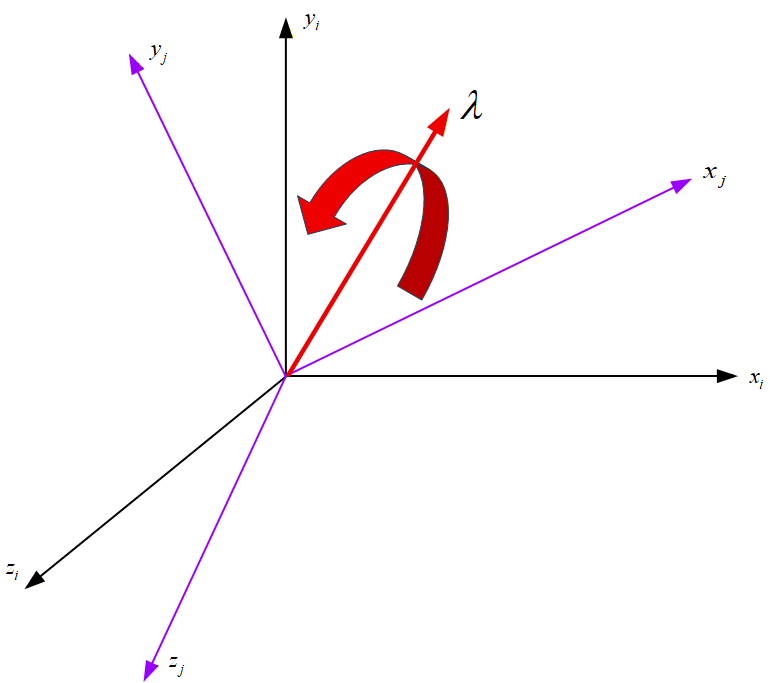
\includegraphics[width=0.6\textwidth]{Figure/简单旋转示意图.png}
    \caption{简单旋转示意图}
    \label{fig:简单旋转示意图}
\end{figure}

\begin{proof}
    由特征多项式的定义：
    \[
    f_{\bm{A}}(\lambda) \triangleq \det(\bm{A}-\lambda\bm{I}_{3})
    \]
    写成显式行列式：
    \[
    =\left|\begin{array}{ccc}
    a_{11}-\lambda & a_{12} & a_{13} \\
    a_{21} & a_{22}-\lambda & a_{23} \\
    a_{31} & a_{32} & a_{33}-\lambda
    \end{array}\right|
    \]

    按第一行余子式展开（cofactor expansion along the first row）：
    \[
    \begin{aligned}
    =&\ (a_{11}-\lambda)\bigl[(a_{22}-\lambda)(a_{33}-\lambda) - a_{23}a_{32}\bigr] \\
    &-\ a_{12}\bigl[a_{21}(a_{33}-\lambda) - a_{23}a_{31}\bigr] \\
    &+\ a_{13}\bigl[a_{21}a_{32} - (a_{22}-\lambda)a_{31}\bigr]
    \end{aligned}
    \]

    记 $M_{kk}$ 为主对角元 $a_{kk}$ 的二阶余子式，即
    \[
    M_{11}=a_{22}a_{33}-a_{23}a_{32},\quad
    M_{22}=a_{11}a_{33}-a_{13}a_{31},\quad
    M_{33}=a_{11}a_{22}-a_{12}a_{21}.
    \]
    将每个二阶行列式用 $M_{kk}$ 与 $\lambda$ 的多项式表示：
    \[
    \begin{aligned}
    (a_{22}-\lambda)(a_{33}-\lambda) - a_{23}a_{32}
        &= M_{11} - (a_{22}+a_{33})\lambda + \lambda^{2} \\
    a_{21}(a_{33}-\lambda) - a_{23}a_{31}
        &= (a_{21}a_{33}-a_{23}a_{31}) - a_{21}\lambda \\
    a_{21}a_{32} - (a_{22}-\lambda)a_{31}
        &= (a_{21}a_{32}-a_{22}a_{31}) + a_{31}\lambda
    \end{aligned}
    \]

    代入并按 $\lambda$ 的幂次合并同类项：
    \[
    \begin{aligned}
    =&\ \underbrace{-\lambda^{3}}_{\text{from }(a_{11}-\lambda)\cdot\lambda^{2}} \\
    &+\ \underbrace{\bigl[a_{11}+(a_{22}+a_{33})\bigr]\lambda^{2}}_{\text{from }(a_{11}-\lambda)\cdot[-(\!a_{22}\!+\!a_{33}\!)\lambda]+\text{其它}} \\
    &-\ \underbrace{\bigl[a_{11}(a_{22}+a_{33})+(a_{22}a_{33}-a_{23}a_{32})-(a_{12}a_{21}+a_{13}a_{31})\bigr]\lambda}_{\text{合并所有 $\lambda^{1}$ 项}} \\
    &+\ \underbrace{(a_{11}a_{22}a_{33}+a_{12}a_{23}a_{31}+a_{13}a_{21}a_{32}-a_{11}a_{23}a_{32}-a_{12}a_{21}a_{33}-a_{13}a_{22}a_{31})}_{\text{常数项}}
    \end{aligned}
    \]

    注意到常数项恰为 $\det\bm{A}$ 的 Sarrus 展开；$\lambda^{1}$ 系数括号中
    \[
    a_{11}(a_{22}+a_{33})+(a_{22}a_{33}-a_{23}a_{32})-(a_{12}a_{21}+a_{13}a_{31})
    =M_{11}+M_{22}+M_{33}=\sum_{k=1}^{3}M_{kk},
    \]
    $\lambda^{2}$ 系数 $a_{11}+a_{22}+a_{33}=\mathrm{tr}(\bm{A})$。故可整理为
    \[
    = -\lambda^{3} + \mathrm{tr}(\bm{A})\,\lambda^{2} - \left(\sum_{k=1}^{3}M_{kk}\right)\lambda + \det(\bm{A}).
    \]

    对于方向余弦矩阵，由 $\bm{A}^{T}\bm{A}=\bm{I}$ 可得
    \[
    M_{11}+M_{22}+M_{33} = \mathrm{tr}(\bm{A}),
    \]
    又由性质 $\det\bm{A}=1$（旋转不改变体积），于是
    \[
    f_{\bm{A}}(\lambda) = -\lambda^{3} + \mathrm{tr}(\bm{A})\,\lambda^{2} - \mathrm{tr}(\bm{A})\,\lambda + 1.
    \]
    将$\lambda=1$代入上式可得：
\[
f_{\bm{A}}(1) = -1 + \mathrm{tr}(\bm{A}) - \mathrm{tr}(\bm{A}) + 1 = 0.
\]
    因此，$\lambda=1$是$f_{\bm{A}}(\lambda)$的一个根，即$\bm{A}$有一个实特征值为1
\end{proof}

从高等代数的角度思考一下这个特征值的意义，我们知道，特征值的意义是：
\begin{equation}
    \bm{A}\bm{\lambda}=\bm{\lambda}
\end{equation}
也就是说，在本次旋转变换中转轴$\bm{\lambda}$并没有发生变化，即转轴朝向不变。

若已知转角$\theta$和转轴$\bm{\lambda}$，那我们怎么得出方向余弦矩阵呢？Kane的书里给出了一种计算方法
\begin{equation}
    \label{eq:方向余弦矩阵计算式}
    \begin{aligned}&a_{11}=\cos\theta+\lambda_1^2(1-\cos\theta)\\&a_{12}=-\lambda_3\sin\theta+\lambda_1\lambda_2(1-\cos\theta)\\&a_{13}=\lambda_2\sin\theta+\lambda_3\lambda_1(1-\cos\theta)\\&a_{21}=\lambda_3\sin\theta+\lambda_1\lambda_2(1-\cos\theta)\\&a_{22}=\cos\theta+\lambda_2^2(1-\cos\theta)\\&a_{23}=-\lambda_1\sin\theta+\lambda_2\lambda_3(1-\cos\theta)\\&a_{31}=-\lambda_2\sin\theta+\lambda_3\lambda_1(1-\cos\theta)\\&a_{32}=\lambda_1\sin\theta+\lambda_2\lambda_3(1-\cos\theta)\\&a_{33}=\cos\theta+\lambda_3^2(1-\cos\theta)
\end{aligned}
\end{equation}
为了方便记忆，引入两个符号$\delta_{ij},\epsilon_{ijk}$
\begin{equation}
    \delta_{ij}\triangleq1-\frac{1}{4}(i-j)^2[5-(i-j)^2]\quad(i,j=1,2,3)
\end{equation}
\begin{equation}
    \epsilon_{ijk}\triangleq\frac{1}{2}(i-j)(j-k)(k-i)\quad(i,j,k=1,2,3)
    \label{eq:epsilon_ijk定义}
\end{equation}
这样式~\eqref{eq:方向余弦矩阵计算式}可以写成：
\begin{equation}
    a_{ij}=\delta_{ij}\cos\theta-\epsilon_{ijk}\lambda_{k}\sin\theta+\lambda_{i}\lambda_{j}(1-\cos\theta)\quad(i,j=1,2,3)
    \label{eq:方向余弦矩阵计算式紧凑}
\end{equation}

那么这个神奇的式子是怎么得到的呢？
\begin{proof}
    我们知道，$\bm{e}_{i|A}=\bm{A}\bm{e}_{i|B}$,然后还有$a_{ij}=\bm{e}_{i|A}\cdot\bm{e}_{j|B}=\bm{e}_{i|B}\cdot(\bm{A}\bm{e}_{j|B})$

    然后又有式~\eqref{eq:simple_rotation_formula}，

$$\bm{e_A} = \bm{e_B}\cos\theta - (\bm{e_B}\times\bm{\lambda})\sin\theta + \bm{\lambda}(\bm{\lambda}\cdot\bm{e_B})(1-\cos\theta)$$
然后再加上$\bm{\lambda}_i \triangleq \bm{\lambda}\cdot\bm{e}_{i|B}=\bm{\lambda}\cdot\bm{e}_{i|A}$
代入即可得到式~\eqref{eq:方向余弦矩阵计算式}
\end{proof}
为了使我们对方向余弦有更好的理解，Kane的书里给出了一个例题。
\begin{example}
    在图~\ref{fig:方向余弦矩阵例题}中，B表示一个均匀矩形块，它是安装在航天器A中的扫描平台的一部分。初始时，B的各条边与固定在A中的单位矢量$\bm{\alpha_1}, \bm{\alpha_2}, \bm{\alpha_3}$平行，随后平台绕B的一条对角线做简单的90度旋转，如示意图所示。设$\bm{I}$为刚体B关于其质心B*的惯性并矢，且定义$\bm{I}_{ij|A}$为$$\bm{I}_{ij|A} \triangleq \bm{\alpha_i} \cdot \bm{I} \cdot \bm{\alpha_j} \quad(i,j=1,2,3)$$问旋转之后的$\bm{I}_{ij|A}\quad(i,j=1,2,3)$为多少？
    \begin{figure}[H]
        \centering
        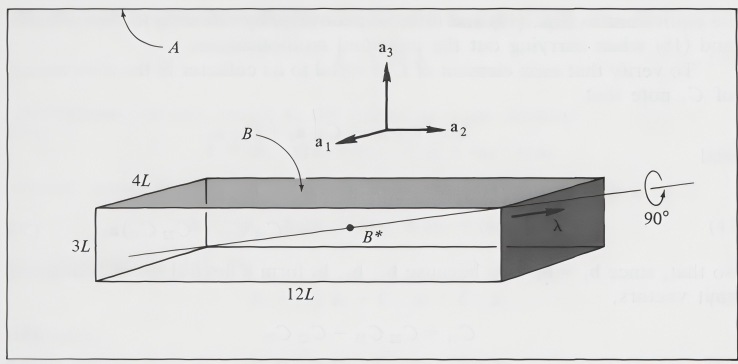
\includegraphics[width=0.8\textwidth]{Figure/例题2.1.png}
        \caption{例题2.1}
        \label{fig:方向余弦矩阵例题}
    \end{figure}
\end{example}
\begin{solution}
    设$\bm{b_1}, \bm{b_2}, \bm{b_3}$为固定在B中的单位向量，旋转前与$\bm{\alpha_1}, \bm{\alpha_2}, \bm{\alpha_3}$相等.

    定义$\bm{I}_{ij|B}\triangleq\bm{b_i} \cdot \bm{I} \cdot \bm{b_j} \quad(i,j=1,2,3)$
    那么$\bm{b_1}$、$\bm{b_2}$和$\bm{b_3}$平行于刚体B对B*点的惯性主轴，因此
    $$\bm{I}_{12|B}=\bm{I}_{21|B}=\bm{I}_{23|B}=\bm{I}_{32|B}=\bm{I}_{31|B}=\bm{I}_{13|B}=0$$
    非主对角线元素均为0，下面计算主对角线元素：
    $$\bm{I}_{11|B}=\frac{m}{12}(12^{2}+3^{2})L^{2}=\frac{153}{12}mL^{2}$$
    $$\bm{I}_{22|B}=\frac{m}{12}(3^2+4^2)L^2=\frac{25}{12}mL^2$$
    $$\bm{I}_{33|B}=\frac{m}{12}(4^2+12^2)L^2=\frac{160}{12}mL^2$$

    于是完整的惯性矩阵：$$\bm{I}_{|B}=\frac{mL^2}{12}\begin{bmatrix}153&0&0\\0&25&0\\0&0&160\end{bmatrix}$$

    转轴对应的单位矢量$\bm{\lambda}$为$$\bm{\lambda}=\frac{4\bm{\alpha_1}+12\bm{\alpha_2}+3\bm{\alpha_3}}{(4^{2}+12^{2}+3^{2})^{1/2}}=\frac{4}{13}\bm{\alpha_1}+\frac{12}{13}\bm{\alpha_2}+\frac{3}{13}\bm{\alpha_3}$$

    由此得到$\bm{\lambda_1}=\frac{4}{13}$、$\bm{\lambda_2}=\frac{12}{13}$、$\bm{\lambda_3}=\frac{3}{13}$
    由式~\eqref{eq:方向余弦矩阵计算式}可得方向余弦矩阵：
    $$\bm{A}=\frac{1}{169}\begin{bmatrix}16&9&168\\87&144&-16\\-144&88&9\end{bmatrix}$$
    又$\bm{I}_{|B}=\bm{A}^\mathrm{T}\bm{I}_{|A} \bm{A}$,所以$\bm{A}\bm{I}_{|B} \bm{A}^\mathrm{T}=\bm{I}_{|A} $
    由此计算出$\bm{I}_{|A}$
    % 注：原转写第3行第2列为 $-1,623,034$，经整数精确验算 $\bm{A}\bm{I}_{|B}\bm{A}^{\mathrm{T}}$ 确认为笔误，已修正为与对称位置一致的 $-1,623,024$。
    $$\begin{aligned}
        &I_{A}=\frac{mL^{2}}{12\times169\times169}\begin{bmatrix}16&9&168\\87&144&-16\\-144&88&9\end{bmatrix}\begin{bmatrix}153&0&0\\0&25&0\\0&0&160\end{bmatrix}\begin{bmatrix}16&87&-144\\9&144&88\\168&-16&9\end{bmatrix}\\&=\frac{mL^{2}}{12\times169\times169}\begin{bmatrix}4,557,033&-184,704&-90,792\\-184,704&1,717,417&-1,623,024\\-90,792&-1,623,024&3,379,168\end{bmatrix}
    \end{aligned}$$

\end{solution}
我发现，有了转轴单位向量还有转角，我们就可以计算出方向余弦矩阵，进而计算出惯性矩阵在不同坐标系下的投影。

    我又发现，方向余弦矩阵的计算在有了转轴向量和转角的情况下是非常机械的，于是使用Python进行一个编程。

    由此，我们不禁反思，既然知道$\bm{\lambda}$还有$\theta$就可以计算出方向余弦矩阵，那我们可不可以抛弃或者说简化矩阵这个形式呢？下面看看欧拉参数。
\newpage
%=============================================================
\section{转轴和转角}\label{sec:simple-rotation}
%=============================================================

\paragraph{用转轴和转角表示的空间运动刚体角速度}

用转轴和转角表示的方向余弦矩阵为
\begin{equation}
    \bm{A}_{ij} = \bm{I}_3 \cos\theta + \tilde{\bm{n}}\sin\theta + \bm{n}\bm{n}^{\mathrm{T}}(1-\cos\theta).
\end{equation}

用转轴和转角表示的相对转动角速度矢量在动系中的投影列阵为
\begin{equation}
    \bm{\omega}_{ij|j} = \bm{n}\dot{\theta} + \sin\theta\,\dot{\tilde{\bm{n}}} - (1-\cos\theta)\tilde{\bm{n}}\dot{\bm{n}}.
\end{equation}

上式两端同时左乘 $\bm{n}^{\mathrm{T}}$ 可得
\begin{equation}
    \dot{\theta} = \bm{n}^{\mathrm{T}}\bm{\omega}_{ij|j}.
\end{equation}

回代后可得
\begin{align}
    \dot{\bm{n}} &= \frac{1}{2\sin\theta}\left[\sin\theta\,\bm{I}_3 - (1+\cos\theta)\tilde{\bm{n}}\right]\tilde{\bm{n}}\bm{\omega}_{ij|j} \notag\\
    &= \frac{1}{2}\left[\bm{I}_3 - \cot(\theta/2)\,\tilde{\bm{n}}\right]\tilde{\bm{n}}\bm{\omega}_{ij|j}.
\end{align}

% ---- 补充视角：Kane 书中的“简单转动”与 Rodrigues 公式 ----
\paragraph*{补充视角：简单转动与 Rodrigues 公式（Kane《Spacecraft Dynamics》）}

以下补充 Kane 书对绕定轴转动的处理：记转轴单位向量为 $\bm{\lambda}$、转角为 $\theta$（对应本节前文的 $\bm{n}$ 与 $\theta$），由 Rodrigues 公式出发可得到与前文一致的方向余弦矩阵。

\begin{mydefinition}{简单转动}
若存在一条称为转轴的直线$L$，其相对于刚体或参考系$A$的取向在整个运动过程中保持不变，和刚体或参考系$B$的取向在整个运动过程中保持不变，则刚体或参考系$B$相对于刚体或参考系$A$的运动称为$B$在$A$中的简单转动。
\end{mydefinition}

设$\bm{a}$为$A$中的一个向量，$\bm{b}$为$B$中的一个向量，且在转动之前与$\bm{a}$重合，则满足如下关系（即Rodrigues公式）：
\begin{equation}\label{eq:simple_rotation_formula}
\bm{b} = \bm{a}\cos\theta - (\bm{a}\times\bm{\lambda})\sin\theta + \bm{\lambda}(\bm{\lambda}\cdot\bm{a})(1-\cos\theta)
\end{equation}

利用叉乘矩阵（定义见数学基础中式~\eqref{eq:矩阵:叉乘矩阵}），由 $\tilde{\bm{\lambda}}\bm{a}=\bm{\lambda}\times\bm{a}$ 可将上式改写为
\begin{equation}\label{eq:simple_rotation_formula矩阵}
\bm{b} = \left[\cos\theta\,\bm{I} + \sin\theta\,\tilde{\bm{\lambda}} + (1-\cos\theta)\,\bm{\lambda}\bm{\lambda}^{\mathrm{T}}\right]\bm{a}.
\end{equation}

如果一个矩阵定义为：
\begin{equation}
    \label{eq:旋转矩阵的代数运算表示}
    \bm{A} \triangleq \bm{U}\cos\theta - (\bm{U}\times\bm{\lambda})\sin\theta + \bm{\lambda}(\bm{\lambda}\cdot\bm{U})(1-\cos\theta)
\end{equation}

则有：
\begin{equation}
    \bm{b} = \bm{a}\cdot\bm{A}
\end{equation}

\begin{proof}
设$\bm{\alpha_{1}}$,$\bm{\alpha_{2}}$为坐标系$A$中的两个单位向量，且满足：
$$
    \bm{\alpha_{1}}\parallel L_{A}
$$
$$
\bm{\alpha_{2}}=\bm{\lambda}\times\bm{\alpha_{1}}
$$

设$\bm{\beta_{1}}$,$\bm{\beta_{2}}$为坐标系$B$中的两个单位向量，且满足：
$$
    \bm{\beta_{1}}\parallel L_{B}
$$
$$
\bm{\beta_{2}}=\bm{\lambda}\times\bm{\beta_{1}}
$$
且满足，当转角$\theta=0$时，有：
$$\bm{a}=\bm{b}$$
$$
    \bm{\alpha_{1}}=\bm{\beta_{1}}
$$
$$
\bm{\alpha_{2}}=\bm{\beta_{2}}
$$
\begin{figure}[H]
    \centering
    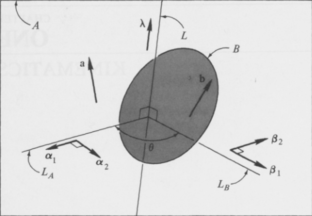
\includegraphics[width=0.8\textwidth]{Figure/1.1简单转动.png}
    \caption{简单转动}
    \label{fig:simple_rotation}
\end{figure}

那么，$\bm{a}$和$\bm{b}$可以表示为：
$$\bm{a}=p\bm{\alpha_{1}}+q\bm{\alpha_{2}}+r\bm{\lambda}$$
$$\bm{b}=p\bm{\beta_{1}}+q\bm{\beta_{2}}+r\bm{\lambda}$$

且有关系：
$$\bm{\beta_{1}}=\cos\theta\bm{\alpha_{1}}+\sin\theta\bm{\alpha_{2}}$$
$$\bm{\beta_{2}}=-\sin\theta\bm{\alpha_{1}}+\cos\theta\bm{\alpha_{2}}$$
代入即可得式子\eqref{eq:simple_rotation_formula}
\end{proof}


%=============================================================
\section{欧拉参数}\label{sec:euler-parameters}
%=============================================================

方向余弦矩阵与转轴和转角的关系式：
\begin{equation}
    \bm{A}_{ij} = \bm{I}_3\cos\theta + \tilde{\bm{n}}\sin\theta + \bm{n}\bm{n}^{\mathrm{T}}(1-\cos\theta).
\end{equation}

三角函数的倍角公式：
\begin{equation}
    \cos\theta = 2\cos^2\frac{\theta}{2}-1,\quad \sin\theta = 2\cos\frac{\theta}{2}\sin\frac{\theta}{2},\quad (1-\cos\theta) = 2\sin^2\frac{\theta}{2}.
\end{equation}

定义四个欧拉参数
\begin{equation}
    \left[\varepsilon_1\quad \varepsilon_2\quad \varepsilon_3\right]^{\mathrm{T}} \triangleq \bm{n}\sin\frac{\theta}{2} =: \tilde{\bm{\varepsilon}},\quad \varepsilon_4 \triangleq \cos\frac{\theta}{2},
\end{equation}

则有如下多项式矩阵形式的方向余弦矩阵
\begin{equation}
    \bm{A}_{ij} = \bm{I}_3(2\varepsilon_4^2 - 1) + 2\tilde{\bm{\varepsilon}}\varepsilon_4 + 2\tilde{\bm{\varepsilon}}\tilde{\bm{\varepsilon}}^{\mathrm{T}}.
\end{equation}

四个欧拉参数
\begin{equation}
    \left[\varepsilon_1\quad \varepsilon_2\quad \varepsilon_3\right]^{\mathrm{T}} \triangleq \bm{n}\sin\frac{\theta}{2} =: \tilde{\bm{\varepsilon}},\quad \varepsilon_4 \triangleq \cos\frac{\theta}{2},
\end{equation}

满足如下约束方程：
\begin{equation}
    \tilde{\bm{\varepsilon}}^2 + \varepsilon_4^2 = \bm{n}^2\sin^2\frac{\theta}{2} + \cos^2\frac{\theta}{2} = \sin^2\frac{\theta}{2} + \cos^2\frac{\theta}{2} = 1.
\end{equation}

则用欧拉参数表示的方向余弦矩阵形式不唯一：
\begin{equation}
    \left\{\begin{aligned}
        \bm{A}_{ij} &= \bm{I}_3(2\varepsilon_4^2 - 1) + 2\tilde{\bm{\varepsilon}}\varepsilon_4 + 2\tilde{\bm{\varepsilon}}\tilde{\bm{\varepsilon}}^{\mathrm{T}},\\
        \bm{A}_{ij} &= \bm{I}_3(1 - 2\tilde{\bm{\varepsilon}}^2) + 2\tilde{\bm{\varepsilon}}\varepsilon_4 + 2\tilde{\bm{\varepsilon}}\tilde{\bm{\varepsilon}}^{\mathrm{T}}.
    \end{aligned}\right.
\end{equation}

用欧拉参数
\begin{equation}
    \left[\varepsilon_1\quad \varepsilon_2\quad \varepsilon_3\right]^{\mathrm{T}} \triangleq \bm{n}\sin\frac{\theta}{2} =: \tilde{\bm{\varepsilon}},\quad \varepsilon_4 \triangleq \cos\frac{\theta}{2}
\end{equation}

表示的方向余弦矩阵
\begin{align}
    \bm{A}_{ij} &= \bm{I}_3(1-2\tilde{\bm{\varepsilon}}^2) + 2\tilde{\bm{\varepsilon}}\varepsilon_4 + 2\tilde{\bm{\varepsilon}}\tilde{\bm{\varepsilon}}^{\mathrm{T}} \notag\\
    &= \begin{bmatrix}
        1-2\varepsilon_2^2-2\varepsilon_3^2 & 2(\varepsilon_1\varepsilon_2-\varepsilon_3\varepsilon_4) & 2(\varepsilon_1\varepsilon_3+\varepsilon_2\varepsilon_4)\\
        2(\varepsilon_2\varepsilon_1+\varepsilon_3\varepsilon_4) & 1-2\varepsilon_3^2-2\varepsilon_1^2 & 2(\varepsilon_2\varepsilon_3-\varepsilon_1\varepsilon_4)\\
        2(\varepsilon_3\varepsilon_1-\varepsilon_2\varepsilon_4) & 2(\varepsilon_3\varepsilon_2+\varepsilon_1\varepsilon_4) & 1-2\varepsilon_1^2-2\varepsilon_2^2
    \end{bmatrix}.
\end{align}

用欧拉参数表示的方向余弦矩阵
\begin{equation}
    \bm{A}_{ij} = \begin{bmatrix}
        1-2\varepsilon_2^2-2\varepsilon_3^2 & 2(\varepsilon_1\varepsilon_2-\varepsilon_3\varepsilon_4) & 2(\varepsilon_1\varepsilon_3+\varepsilon_2\varepsilon_4)\\
        2(\varepsilon_2\varepsilon_1+\varepsilon_3\varepsilon_4) & 1-2\varepsilon_3^2-2\varepsilon_1^2 & 2(\varepsilon_2\varepsilon_3-\varepsilon_1\varepsilon_4)\\
        2(\varepsilon_3\varepsilon_1-\varepsilon_2\varepsilon_4) & 2(\varepsilon_3\varepsilon_2+\varepsilon_1\varepsilon_4) & 1-2\varepsilon_1^2-2\varepsilon_2^2
    \end{bmatrix},
\end{equation}

四个欧拉参数满足模为 1 的约束方程，即
\begin{equation}
    \varepsilon_1^2 + \varepsilon_2^2 + \varepsilon_3^2 + \varepsilon_4^2 = 1.
\end{equation}

由
\begin{equation}
    \tilde{\bm{\omega}}_{ij|j} = \bm{A}_{ij}^{\mathrm{T}}\dot{\bm{A}}_{ij}
\end{equation}

可得用欧拉参数及其导数表示的 $\bm{\omega}_{ij|j}$ 的表达式。

用欧拉参数及其导数表示的 $\bm{\omega}_{ij|j}$ 的表达式为
\begin{equation}
    \bm{\omega}_{ij|j} = 2\begin{bmatrix}
        \varepsilon_4 & \varepsilon_3 & -\varepsilon_2 & -\varepsilon_1\\
        -\varepsilon_3 & \varepsilon_4 & \varepsilon_1 & -\varepsilon_2\\
        \varepsilon_2 & -\varepsilon_1 & \varepsilon_4 & -\varepsilon_3
    \end{bmatrix}
    \begin{bmatrix}
        \dot{\varepsilon}_1\\
        \dot{\varepsilon}_2\\
        \dot{\varepsilon}_3\\
        \dot{\varepsilon}_4
    \end{bmatrix}
    = 2\left[\varepsilon_4\bm{I}_3 - \tilde{\bm{\varepsilon}}\quad -\tilde{\bm{\varepsilon}}\right]\dot{\bm{\varepsilon}} =: \bm{H}_{\mathrm{EP}}\dot{\bm{\varepsilon}}.
\end{equation}

进一步可得
\begin{align}
    \bm{\omega}_{ij|i} &= \bm{A}_{ij}\bm{\omega}_{ij|j} = 2\left[\varepsilon_4\bm{I}_3 + \tilde{\bm{\varepsilon}}\quad -\tilde{\bm{\varepsilon}}\right]\dot{\bm{\varepsilon}},\\
    \frac{\partial\bm{\omega}_{ij|i}}{\partial\bm{\varepsilon}} &= 2\begin{bmatrix}
        -\dot{\varepsilon}_4 & -\dot{\varepsilon}_3 & \dot{\varepsilon}_2 & \dot{\varepsilon}_1\\
        \dot{\varepsilon}_3 & -\dot{\varepsilon}_4 & -\dot{\varepsilon}_1 & \dot{\varepsilon}_2\\
        -\dot{\varepsilon}_2 & \dot{\varepsilon}_1 & -\dot{\varepsilon}_4 & \dot{\varepsilon}_3
    \end{bmatrix}
    = 2\left[-\dot{\varepsilon}_4\bm{I}_3 + \tilde{\dot{\bm{\varepsilon}}}\quad \dot{\tilde{\bm{\varepsilon}}}\right].
\end{align}

\paragraph*{推导过程}

\begin{align}
    (\omega_x)_{ij|j} &= a_{13}\dot{a}_{12} + a_{23}\dot{a}_{22} + a_{33}\dot{a}_{32}\notag\\
    &= \left[4\varepsilon_1(\varepsilon_1\varepsilon_4 - \varepsilon_2\varepsilon_3) + 2\varepsilon_4\right]\dot{\varepsilon}_1\notag\\
    &\quad + \left[4\varepsilon_2(\varepsilon_1\varepsilon_4 - \varepsilon_2\varepsilon_3) + 2\varepsilon_3\right]\dot{\varepsilon}_2\notag\\
    &\quad + \left[4\varepsilon_3(\varepsilon_1\varepsilon_4 - \varepsilon_2\varepsilon_3) - 2\varepsilon_2\right]\dot{\varepsilon}_3\notag\\
    &\quad + \left[4\varepsilon_4(\varepsilon_1\varepsilon_4 - \varepsilon_2\varepsilon_3) - 2\varepsilon_1\right]\dot{\varepsilon}_4\notag\\
    &= 2\varepsilon_4\dot{\varepsilon}_1 + 2\varepsilon_3\dot{\varepsilon}_2 - 2\varepsilon_2\dot{\varepsilon}_3 - 2\varepsilon_1\dot{\varepsilon}_4.
\end{align}

\begin{equation}
    \bm{A}_{ij} = \begin{bmatrix}
        1-2\varepsilon_2^2-2\varepsilon_3^2 & 2(\varepsilon_1\varepsilon_2-\varepsilon_3\varepsilon_4) & 2(\varepsilon_1\varepsilon_3+\varepsilon_2\varepsilon_4)\\
        2(\varepsilon_2\varepsilon_1+\varepsilon_3\varepsilon_4) & 1-2\varepsilon_3^2-2\varepsilon_1^2 & 2(\varepsilon_2\varepsilon_3-\varepsilon_1\varepsilon_4)\\
        2(\varepsilon_3\varepsilon_1-\varepsilon_2\varepsilon_4) & 2(\varepsilon_3\varepsilon_2+\varepsilon_1\varepsilon_4) & 1-2\varepsilon_1^2-2\varepsilon_2^2
    \end{bmatrix}
    = \begin{bmatrix}
        a_{11} & a_{12} & a_{13}\\
        a_{21} & a_{22} & a_{23}\\
        a_{31} & a_{32} & a_{33}
    \end{bmatrix}.
\end{equation}

\begin{align}
    \tilde{\bm{\omega}}_{ij|j} &= \bm{A}_{ij}^{\mathrm{T}}\dot{\bm{A}}_{ij}\notag\\
    &= \begin{bmatrix}
        a_{11} & a_{21} & a_{31}\\
        a_{12} & a_{22} & a_{32}\\
        a_{13} & a_{23} & a_{33}
    \end{bmatrix}
    \begin{bmatrix}
        \dot{a}_{11} & \dot{a}_{12} & \dot{a}_{13}\\
        \dot{a}_{21} & \dot{a}_{22} & \dot{a}_{23}\\
        \dot{a}_{31} & \dot{a}_{32} & \dot{a}_{33}
    \end{bmatrix}\notag\\
    &= \begin{bmatrix}
        0 & -(\omega_z)_{ij|j} & (\omega_y)_{ij|j}\\
        (\omega_z)_{ij|j} & 0 & -(\omega_x)_{ij|j}\\
        -(\omega_y)_{ij|j} & (\omega_x)_{ij|j} & 0
    \end{bmatrix}.
\end{align}

\begin{equation}
    1 = \varepsilon_1^2 + \varepsilon_2^2 + \varepsilon_3^2 + \varepsilon_4^2.
\end{equation}

\begin{equation}
    0 = 2(\varepsilon_1\dot{\varepsilon}_1 + \varepsilon_2\dot{\varepsilon}_2 + \varepsilon_3\dot{\varepsilon}_3 + \varepsilon_4\dot{\varepsilon}_4).
\end{equation}

%-------------------------------------------------------------
\paragraph{由角速度列阵反求欧拉参数对时间的一阶导数}
%-------------------------------------------------------------

用欧拉参数及其导数表示的 $\bm{\omega}_{ij|j}$ 的表达式为
\begin{equation}
    \bm{\omega}_{ij|j} = 2\begin{bmatrix}
        \varepsilon_4 & \varepsilon_3 & -\varepsilon_2 & -\varepsilon_1\\
        -\varepsilon_3 & \varepsilon_4 & \varepsilon_1 & -\varepsilon_2\\
        \varepsilon_2 & -\varepsilon_1 & \varepsilon_4 & -\varepsilon_3
    \end{bmatrix}
    \begin{bmatrix}
        \dot{\varepsilon}_1\\
        \dot{\varepsilon}_2\\
        \dot{\varepsilon}_3\\
        \dot{\varepsilon}_4
    \end{bmatrix}
    = 2\left[\varepsilon_4\bm{I}_3 - \tilde{\bm{\varepsilon}}\quad -\tilde{\bm{\varepsilon}}\right]\dot{\bm{\varepsilon}} =: \bm{H}_{\mathrm{EP}}\dot{\bm{\varepsilon}}.
\end{equation}

由上式可得用相对转动角速度表示的欧拉参数一阶导数，即
\begin{equation}
    \dot{\bm{\varepsilon}} = \frac{1}{2}\begin{bmatrix}
        \varepsilon_4\bm{I}_3 + \tilde{\bm{\varepsilon}}\\
        -\tilde{\bm{\varepsilon}}^{\mathrm{T}}
    \end{bmatrix}
    \bm{\omega}_{ij|j}.
\end{equation}

\paragraph*{推导过程}

\begin{equation}
    \bm{\omega}_{ij|j} = 2\begin{bmatrix}
        \varepsilon_4 & \varepsilon_3 & -\varepsilon_2 & -\varepsilon_1\\
        -\varepsilon_3 & \varepsilon_4 & \varepsilon_1 & -\varepsilon_2\\
        \varepsilon_2 & -\varepsilon_1 & \varepsilon_4 & -\varepsilon_3
    \end{bmatrix}
    \begin{bmatrix}
        \dot{\varepsilon}_1\\
        \dot{\varepsilon}_2\\
        \dot{\varepsilon}_3\\
        \dot{\varepsilon}_4
    \end{bmatrix},
\end{equation}

\begin{equation}
    0 = 2(\varepsilon_1\dot{\varepsilon}_1 + \varepsilon_2\dot{\varepsilon}_2 + \varepsilon_3\dot{\varepsilon}_3 + \varepsilon_4\dot{\varepsilon}_4),
\end{equation}

\begin{equation}
    \begin{bmatrix}
        \bm{\omega}_{ij|j}\\
        0
    \end{bmatrix}
    = 2\begin{bmatrix}
        \varepsilon_4 & \varepsilon_3 & -\varepsilon_2 & -\varepsilon_1\\
        -\varepsilon_3 & \varepsilon_4 & \varepsilon_1 & -\varepsilon_2\\
        \varepsilon_2 & -\varepsilon_1 & \varepsilon_4 & -\varepsilon_3\\
        \varepsilon_1 & \varepsilon_2 & \varepsilon_3 & \varepsilon_4
    \end{bmatrix}
    \begin{bmatrix}
        \dot{\varepsilon}_1\\
        \dot{\varepsilon}_2\\
        \dot{\varepsilon}_3\\
        \dot{\varepsilon}_4
    \end{bmatrix}
    =: 2\bar{\bm{H}}_{\mathrm{EP}}\dot{\bm{\varepsilon}}.
\end{equation}

\begin{equation}
    \begin{bmatrix}
        \bm{\omega}_{ij|j}\\
        0
    \end{bmatrix}
    = 2\bar{\bm{H}}_{\mathrm{EP}}\dot{\bm{\varepsilon}},\quad
    \bar{\bm{H}}_{\mathrm{EP}} = \begin{bmatrix}
        \varepsilon_4 & \varepsilon_3 & -\varepsilon_2 & -\varepsilon_1\\
        -\varepsilon_3 & \varepsilon_4 & \varepsilon_1 & -\varepsilon_2\\
        \varepsilon_2 & -\varepsilon_1 & \varepsilon_4 & -\varepsilon_3\\
        \varepsilon_1 & \varepsilon_2 & \varepsilon_3 & \varepsilon_4
    \end{bmatrix}.
\end{equation}

\begin{equation}
    \bar{\bm{H}}_{\mathrm{EP}}^{\mathrm{T}}\bar{\bm{H}}_{\mathrm{EP}} = \begin{bmatrix}
        \varepsilon_4 & -\varepsilon_3 & \varepsilon_2 & \varepsilon_1\\
        \varepsilon_3 & \varepsilon_4 & -\varepsilon_1 & \varepsilon_2\\
        -\varepsilon_2 & \varepsilon_1 & \varepsilon_4 & \varepsilon_3\\
        -\varepsilon_1 & -\varepsilon_2 & -\varepsilon_3 & \varepsilon_4
    \end{bmatrix}
    \begin{bmatrix}
        \varepsilon_4 & \varepsilon_3 & -\varepsilon_2 & -\varepsilon_1\\
        -\varepsilon_3 & \varepsilon_4 & \varepsilon_1 & -\varepsilon_2\\
        \varepsilon_2 & -\varepsilon_1 & \varepsilon_4 & -\varepsilon_3\\
        \varepsilon_1 & \varepsilon_2 & \varepsilon_3 & \varepsilon_4
    \end{bmatrix}
    = \bm{I}_4.
\end{equation}

\begin{equation}
    \begin{bmatrix}
        \bm{\omega}_{ij|j}\\
        0
    \end{bmatrix}
    = 2\bar{\bm{H}}_{\mathrm{EP}}\dot{\bm{\varepsilon}},\quad
    \bar{\bm{H}}_{\mathrm{EP}} = \begin{bmatrix}
        \varepsilon_4 & \varepsilon_3 & -\varepsilon_2 & -\varepsilon_1\\
        -\varepsilon_3 & \varepsilon_4 & \varepsilon_1 & -\varepsilon_2\\
        \varepsilon_2 & -\varepsilon_1 & \varepsilon_4 & -\varepsilon_3\\
        \varepsilon_1 & \varepsilon_2 & \varepsilon_3 & \varepsilon_4
    \end{bmatrix},\quad
    \bar{\bm{H}}_{\mathrm{EP}}^{\mathrm{T}}\bar{\bm{H}}_{\mathrm{EP}} = \bm{I}_4.
\end{equation}

因此
\begin{align}
    \dot{\bm{\varepsilon}} &= \frac{1}{2}\bar{\bm{H}}_{\mathrm{EP}}^{\mathrm{T}}
    \begin{bmatrix}
        \bm{\omega}_{ij|j}\\
        0
    \end{bmatrix}\notag\\
    &= \frac{1}{2}\begin{bmatrix}
        \varepsilon_4 & -\varepsilon_3 & \varepsilon_2 & \varepsilon_1\\
        \varepsilon_3 & \varepsilon_4 & -\varepsilon_1 & \varepsilon_2\\
        -\varepsilon_2 & \varepsilon_1 & \varepsilon_4 & \varepsilon_3\\
        -\varepsilon_1 & -\varepsilon_2 & -\varepsilon_3 & \varepsilon_4
    \end{bmatrix}
    \begin{bmatrix}
        \bm{\omega}_{ij|j}\\
        0
    \end{bmatrix}
    = \frac{1}{2}\begin{bmatrix}
        \varepsilon_4\bm{I}_3 + \tilde{\bm{\varepsilon}}\\
        -\tilde{\bm{\varepsilon}}^{\mathrm{T}}
    \end{bmatrix}
    \bm{\omega}_{ij|j}.
\end{align}

%=============================================================
%
% ---- 补充视角：Kane 书中的欧拉参数性质、转换与应用 ----
\paragraph*{补充视角：欧拉参数的性质、转换与应用（Kane《Spacecraft Dynamics》）}

以下为 Kane 书视角的补充。记号对应：转轴单位向量 $\bm{\lambda}$ 对应前文 $\bm{n}$；$(\epsilon_1,\epsilon_2,\epsilon_3)$、$\epsilon_4$ 即前文的欧拉参数 $\varepsilon_1,\dots,\varepsilon_4$；方向余弦矩阵 $[a_{ij}]$ 对应前文 $\bm{A}_{ij}$。

欧拉参数（Euler Parameters），也叫欧拉四元数，也可以简称四元数，下面我们来看看，怎么用欧拉参数来描述转动。

上面我们知道，单纯描述转动过程是与外形无关的。描述一个转动过程只需要两个量：转轴和转角。于是我们可以用一个单位向量$\bm{\lambda}$来表示转轴，用一个实数$\theta$来表示转角。于是我们可以定义欧拉参数：
\begin{mydefinition}{欧拉参数}
    设$\bm{\lambda}$为转轴单位向量，$\theta$为转角，则欧拉参数定义为：
    \begin{equation}
        \label{eq:欧拉参数定义}
        \begin{aligned}
            &\bm{\epsilon} \triangleq \bm{\lambda}\sin \frac{\theta}{2}\\
            &\epsilon_i \triangleq \bm{\epsilon} \cdot \bm{a}_i=\bm{\epsilon} \cdot \bm{b}_i\quad(i=1,2,3)\\
            &\epsilon_4 \triangleq \cos \frac{\theta}{2}
        \end{aligned}
    \end{equation}

\end{mydefinition}



上面我们讨论了方向余弦矩阵中的9个元素满足六个约束关系，也就是独立的坐标其实只有三个，而欧拉参数中有四个元素，从物理的角度，描述同一个转动过程，欧拉参数一定满足一个约束关系，这个关系是什么？从数学的角度十分直观：
\begin{equation}\label{eq:欧拉参数归一化}
    \bm{\epsilon}^2+\epsilon_4^2=\epsilon_1^2+\epsilon_2^2+\epsilon_3^2+\epsilon_4^2=1
\end{equation}

我们知道，欧拉参数和方向余弦都是描述转动的工具，那么在描述同一个转动时，两者之间一定存在关系，Kane在书中给出：
\begin{equation}
    \begin{aligned}
        a_{11} &= \epsilon_1^2 - \epsilon_2^2 - \epsilon_3^2 + \epsilon_4^2 = 1 - 2\epsilon_2^2 - 2\epsilon_3^2,\\
        a_{12} &= 2(\epsilon_1 \epsilon_2 - \epsilon_3 \epsilon_4),\\
        a_{13} &= 2(\epsilon_3 \epsilon_1 + \epsilon_2 \epsilon_4),\\
        a_{21} &= 2(\epsilon_1 \epsilon_2 + \epsilon_3 \epsilon_4),\\
        a_{22} &= \epsilon_2^2 - \epsilon_3^2 - \epsilon_1^2 + \epsilon_4^2 = 1 - 2\epsilon_3^2 - 2\epsilon_1^2,\\
        a_{23} &= 2(\epsilon_2 \epsilon_3 - \epsilon_1 \epsilon_4),\\
        a_{31} &= 2(\epsilon_3 \epsilon_1 - \epsilon_2 \epsilon_4),\\
        a_{32} &= 2(\epsilon_2 \epsilon_3 + \epsilon_1 \epsilon_4),\\
        a_{33} &= \epsilon_3^2 - \epsilon_1^2 - \epsilon_2^2 + \epsilon_4^2 = 1 - 2\epsilon_1^2 - 2\epsilon_2^2.
    \end{aligned}
    \label{eq:欧拉参数转方向余弦}
\end{equation}
欧拉参数也可以由方向余弦给出：
\begin{equation}
    \begin{aligned}
        \epsilon_{1} &= \frac{a_{32}-a_{23}}{4\epsilon_4},\\
        \epsilon_{2} &= \frac{a_{13}-a_{31}}{4\epsilon_4},\\
        \epsilon_{3} &= \frac{a_{21}-a_{12}}{4\epsilon_4},\\
        \epsilon_4 &= \frac{1}{2}\left(1+a_{11}+a_{22}+a_{33}\right)^{1/2}.
    \end{aligned}
    \label{eq:方向余弦转欧拉参数}
\end{equation}

对于转轴有：
\begin{equation}
    \bm{\lambda}=\frac{\epsilon_1\mathbf{a}_1+\epsilon_2\mathbf{a}_2+\epsilon_3\mathbf{a}_3}{(\epsilon_1^2+\epsilon_2^2+\epsilon_3^2)^{1/2}}
    \label{eq:欧拉参数得转轴}
\end{equation}

对于转角有：
\begin{equation}
    \theta=2\arccos\epsilon_4 \quad \theta \in [0,\pi]
    \label{eq:欧拉参数得转角}
\end{equation}
简单转动的公式也迎来了欧拉参数的形式：
\begin{equation}
    \mathbf{b}=\mathbf{a}+2[\epsilon_4 \bm{\epsilon}\times\mathbf{a}+\bm{\epsilon}\times(\bm{\epsilon}\times\mathbf{a})]
    \label{eq:转动公式的欧拉参数形式}
\end{equation}
利用叉乘矩阵，$\bm{\epsilon}\times\mathbf{a}=\tilde{\bm{\epsilon}}\,\mathbf{a}$、$\bm{\epsilon}\times(\bm{\epsilon}\times\mathbf{a})=\tilde{\bm{\epsilon}}^{\,2}\mathbf{a}$，故上式可写成
\begin{equation}
    \mathbf{b}=\left[\bm{I}+2\epsilon_4\,\tilde{\bm{\epsilon}}+2\tilde{\bm{\epsilon}}^{\,2}\right]\mathbf{a}.
    \label{eq:转动公式的欧拉参数形式矩阵}
\end{equation}
那么，式~\eqref{eq:欧拉参数转方向余弦}、式~\eqref{eq:方向余弦转欧拉参数}、式~\eqref{eq:欧拉参数得转轴}、式~\eqref{eq:欧拉参数得转角}和式~\eqref{eq:转动公式的欧拉参数形式}是怎么得到的呢？下面给出Kane书中的证明。

\begin{proof}
\textbf{（一）式~\eqref{eq:欧拉参数转方向余弦} 的推导。}  利用 $\bm{\lambda}$ 为单位向量，故 $1=\lambda_1^2+\lambda_2^2+\lambda_3^2$，结合式~\eqref{eq:欧拉参数归一化} 的 $\epsilon_4^2+\epsilon_1^2+\epsilon_2^2+\epsilon_3^2=1$，有
$$
\epsilon_i^2=\frac{1-\cos\theta}{2}\,\lambda_i^{2},\quad 1-2\epsilon_j^2-2\epsilon_k^2=\lambda_i^2(1-\cos\theta)+\cos\theta \quad (i,j,k\text{ 互不相同})
$$
代入式~\eqref{eq:欧拉参数转方向余弦} 即可得 $a_{11},a_{22},a_{33}$ 的表达。再利用 $\sin\theta=2\sin(\theta/2)\cos(\theta/2)$ 以及 $\epsilon_i=\lambda_i\sin(\theta/2)$，$\epsilon_4=\cos(\theta/2)$，可把 6 个非对角元全部表示为 $\epsilon_1,\epsilon_2,\epsilon_3,\epsilon_4$ 的二次齐次式，整理即得式~\eqref{eq:欧拉参数转方向余弦}。

\textbf{（二）式~\eqref{eq:方向余弦转欧拉参数} 的推导。}  把式~\eqref{eq:欧拉参数转方向余弦} 中三个对角元相加：
$$
a_{11}+a_{22}+a_{33}=3-4(\epsilon_1^2+\epsilon_2^2+\epsilon_3^2)=3-4(1-\epsilon_4^2)=4\epsilon_4^2-1
$$
故 $\epsilon_4^2=\dfrac{1+a_{11}+a_{22}+a_{33}}{4}$。由于 $\epsilon_4=\cos(\theta/2)$，$\theta\in[0,\pi]$，$\cos(\theta/2)\geq 0$，故取正根
$$
\epsilon_4=\frac{1}{2}(1+a_{11}+a_{22}+a_{33})^{1/2}
$$
将 $a_{ij}-a_{ji}$（反对角差）展开，结合 $\epsilon_4$ 的非零性可得
$$
\epsilon_1=\frac{a_{32}-a_{23}}{4\epsilon_4},\quad \epsilon_2=\frac{a_{13}-a_{31}}{4\epsilon_4},\quad \epsilon_3=\frac{a_{21}-a_{12}}{4\epsilon_4}
$$
即式~\eqref{eq:方向余弦转欧拉参数}。

\textbf{（三）式~\eqref{eq:欧拉参数得转轴} 的推导。}  由式~\eqref{eq:欧拉参数定义} 知
$$
\bm{\lambda}\sin\frac{\theta}{2}=\bm{\epsilon}
$$
而由欧拉参数的归一化 $\epsilon_4^2+\epsilon_1^2+\epsilon_2^2+\epsilon_3^2=1$ 与 $\epsilon_4=\cos(\theta/2)$ 可得
$$
\sin\frac{\theta}{2}=(\epsilon_1^2+\epsilon_2^2+\epsilon_3^2)^{1/2}
$$
故
$$
\bm{\lambda}=\frac{\bm{\epsilon}}{(\epsilon_1^2+\epsilon_2^2+\epsilon_3^2)^{1/2}}=\frac{\epsilon_1\mathbf{a}_1+\epsilon_2\mathbf{a}_2+\epsilon_3\mathbf{a}_3}{(\epsilon_1^2+\epsilon_2^2+\epsilon_3^2)^{1/2}}
$$
即式~\eqref{eq:欧拉参数得转轴}。

\textbf{（四）式~\eqref{eq:欧拉参数得转角} 的推导。}  直接由 $\epsilon_4=\cos(\theta/2)$ 取逆：
$$
\theta=2\arccos\epsilon_4,\quad \theta\in[0,\pi]
$$
此即式~\eqref{eq:欧拉参数得转角}。注意 $\theta$ 的取值范围限制在 $[0,\pi]$ 是因为 $\cos$ 在 $[0,\pi]$ 上单调且与 $[0,2\pi]$ 的转角一一对应（$\theta$ 与 $-\theta$ 等价，反向旋转可由 $\bm{\lambda}$ 翻转吸收）。

\textbf{（五）式~\eqref{eq:转动公式的欧拉参数形式} 的推导。}  由式~\eqref{eq:simple_rotation_formula}：
$$
\mathbf{b}=\mathbf{a}+\bm{\lambda}\times\mathbf{a}\sin\theta+\bm{\lambda}\times(\bm{\lambda}\times\mathbf{a})(1-\cos\theta)
$$
利用 $\sin\theta=2\sin(\theta/2)\cos(\theta/2)=2\epsilon\sin(\theta/2)\cdot\epsilon_4$（其中 $\epsilon\sin(\theta/2)=|\bm{\lambda}|\sin(\theta/2)=1\cdot\sin(\theta/2)$），以及 $1-\cos\theta=2\sin^2(\theta/2)=2\epsilon^2$ 代入得
$$
\begin{aligned}
\mathbf{b}&=\mathbf{a}+2\epsilon_4\,\bm{\epsilon}\times\mathbf{a}+2\bm{\epsilon}\times(\bm{\epsilon}\times\mathbf{a})\\
&=\mathbf{a}+2\bigl[\epsilon_4\,\bm{\epsilon}\times\mathbf{a}+\bm{\epsilon}\times(\bm{\epsilon}\times\mathbf{a})\bigr]
\end{aligned}
$$
这正是式~\eqref{eq:转动公式的欧拉参数形式}，证毕。
\end{proof}
\blocksep
\begin{example}
    \begin{figure}[H]
        \centering
        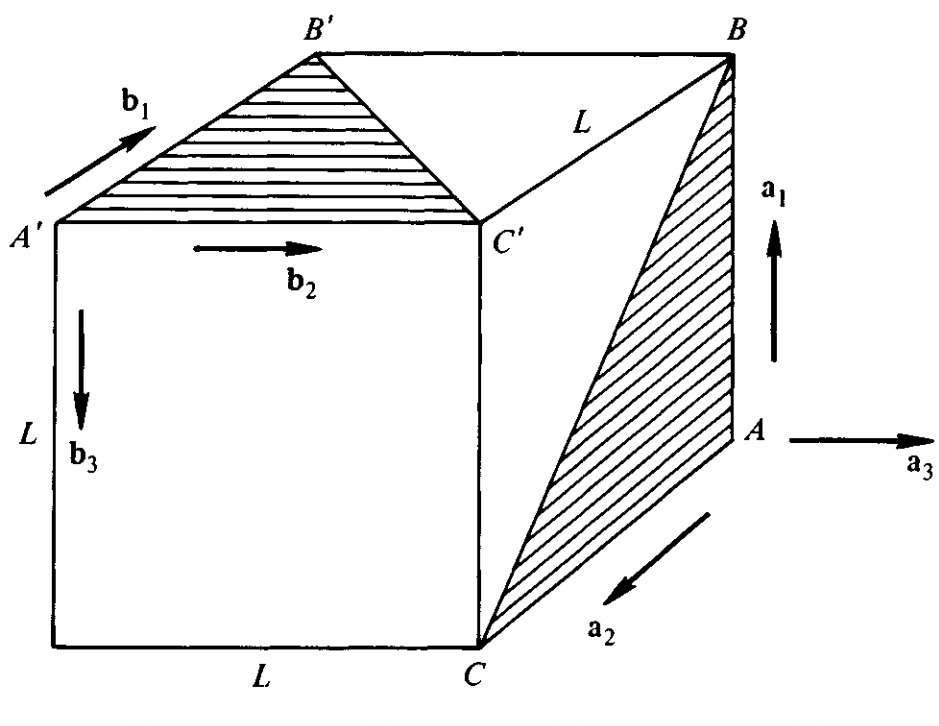
\includegraphics[width=0.8\textwidth]{Figure/例题2.2.png}
        \caption{例题2.2}
        \label{fig:欧拉参数例题}
    \end{figure}

图~\ref{fig:欧拉参数例题} 中的三角形 $ABC$ 可通过如下两步进入位置 $A'B'C'$：先将 $A$ 平移到 $A'$（保持三角形朝向不变），再以固定在 $A'$ 的 $A$ 点为支点作一个简单旋转。设 $\mathbf{a}_i$ 和 $\mathbf{b}_i$ ($i=1,2,3$) 沿如图所示方向取单位向量，使得旋转前 $\mathbf{a}_i=\mathbf{b}_i\,(i=1,2,3)$。求转轴单位向量 $\bm{\lambda}$ 和相应的转角 $\theta$。
\end{example}

\begin{solution}
按式~\eqref{eq:方向余弦转欧拉参数} 求 $\epsilon_i$ 时，需要先求 $a_{ij}=\mathbf{a}_i\cdot\mathbf{b}_j$。由图~\ref{fig:欧拉参数例题} 中的几何关系可知
$$
a_{11}=\mathbf{a}_1\cdot\mathbf{b}_1=0,\quad
a_{22}=\mathbf{a}_2\cdot\mathbf{b}_2=0,\quad
a_{33}=\mathbf{a}_3\cdot\mathbf{b}_3=0,
$$
$$
a_{12}=\mathbf{a}_1\cdot\mathbf{b}_2=1,\quad a_{21}=-1;\quad
a_{13}=-1,\quad a_{31}=0;\quad
a_{23}=0,\quad a_{32}=1.
$$
代入式~\eqref{eq:方向余弦转欧拉参数}：
$$
\epsilon_4=\frac{1}{2}\bigl(1+0+0+0\bigr)^{1/2}=\frac{1}{2}
$$
$$
\epsilon_1=\frac{\mathbf{a}_3\cdot\mathbf{b}_2-\mathbf{a}_2\cdot\mathbf{b}_3}{4\cdot\tfrac{1}{2}}=\frac{1-0}{2}=\frac{1}{2}
$$
$$
\epsilon_2=\frac{\mathbf{a}_1\cdot\mathbf{b}_3-\mathbf{a}_3\cdot\mathbf{b}_1}{4\cdot\tfrac{1}{2}}=\frac{-1-0}{2}=-\frac{1}{2}
$$
$$
\epsilon_3=\frac{\mathbf{a}_2\cdot\mathbf{b}_1-\mathbf{a}_1\cdot\mathbf{b}_2}{4\cdot\tfrac{1}{2}}=\frac{-1-0}{2}=-\frac{1}{2}
$$
再由式~\eqref{eq:欧拉参数得转轴}，$\sin(\theta/2)=(\epsilon_1^2+\epsilon_2^2+\epsilon_3^2)^{1/2}=(3/4)^{1/2}$，故
$$
\bm{\lambda}=\frac{\bm{\epsilon}}{(\epsilon_1^2+\epsilon_2^2+\epsilon_3^2)^{1/2}}=\frac{\tfrac{1}{2}\mathbf{a}_1-\tfrac{1}{2}\mathbf{a}_2-\tfrac{1}{2}\mathbf{a}_3}{(3/4)^{1/2}}=\frac{\mathbf{a}_1-\mathbf{a}_2-\mathbf{a}_3}{\sqrt{3}}
$$
由式~\eqref{eq:欧拉参数得转角}：
$$
\theta=2\cos^{-1}\epsilon_4=2\cos^{-1}\tfrac{1}{2}=\frac{2\pi}{3}\ \mathrm{rad}
$$
\end{solution}

%=============================================================
\section{欧拉角}\label{sec:euler-angles}
%=============================================================

\paragraph{体内ZXZ转动（经典欧拉角）}

\begin{figure}[H]
    \centering
    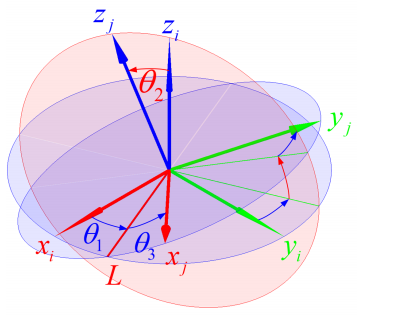
\includegraphics[width=0.8\textwidth]{Figure/体内ZXZ转动（经典欧拉角）示意图.png}
    \caption{体内ZXZ转动（经典欧拉角）示意图}
    \label{fig:chapter7_euler_ZXZ}
\end{figure}

从 $i$ 系到 $j$ 系的相对转动解读为绕连体坐标系（动系）坐标轴的三次相继转动，转轴分别为 $Z$、$X$、$Z$，转角分别为 $\theta_1$、$\theta_2$、$\theta_3$。

\begin{enumerate}
    \item $\theta_1$: 转轴 $z_i$，进动角（$\psi$）
    \item $\theta_2$: 转轴 $L$，章动角（$\theta$）
    \item $\theta_3$: 转轴 $z_j$，自转角（$\varphi$）
\end{enumerate}

坐标变换矩阵：
\begin{equation}
    \bm{A}_{ij} = \bm{A}_z(\theta_1)\bm{A}_x(\theta_2)\bm{A}_z(\theta_3).
\end{equation}

体内ZXZ转动与坐标变换矩阵的关系\quad 由转角表示的坐标变换矩阵：
\begin{align}
    \bm{A}_{ij} &= \bm{A}_z(\theta_1)\bm{A}_x(\theta_2)\bm{A}_z(\theta_3)\notag\\
    &= \begin{bmatrix}
        \cos\theta_1 & -\sin\theta_1 & 0\\
        \sin\theta_1 & \cos\theta_1 & 0\\
        0 & 0 & 1
    \end{bmatrix}
    \begin{bmatrix}
        1 & 0 & 0\\
        0 & \cos\theta_2 & -\sin\theta_2\\
        0 & \sin\theta_2 & \cos\theta_2
    \end{bmatrix}
    \begin{bmatrix}
        \cos\theta_3 & -\sin\theta_3 & 0\\
        \sin\theta_3 & \cos\theta_3 & 0\\
        0 & 0 & 1
    \end{bmatrix}\notag\\
    &= \begin{bmatrix}
        c_1c_3 - s_1c_2s_3 & -c_1s_3 - s_1c_2c_3 & s_1s_2\\
        s_1c_3 + c_1c_2s_3 & c_1c_2c_3 - s_1s_3 & -c_1s_2\\
        s_2s_3 & s_2c_3 & c_2
    \end{bmatrix}.
\end{align}

由坐标变换矩阵反求转角：
\begin{equation}
    \bm{A}_{ij} = \begin{bmatrix}
        c_1c_3 - s_1c_2s_3 & -c_1s_3 - s_1c_2c_3 & s_1s_2\\
        s_1c_3 + c_1c_2s_3 & c_1c_2c_3 - s_1s_3 & -c_1s_2\\
        s_2s_3 & s_2c_3 & c_2
    \end{bmatrix}
    = \begin{bmatrix}
        a_{11} & a_{12} & a_{13}\\
        a_{21} & a_{22} & a_{23}\\
        a_{31} & a_{32} & a_{33}
    \end{bmatrix}.
\end{equation}

由上式可知，(I) 当 $c_2 = a_{33} \approx 1$ 时，$s_2 \approx 0$，此时
\begin{equation}
    \bm{A}_{ij} = \begin{bmatrix}
        c_1c_3 - s_1s_3 & -c_1s_3 - s_1c_3 & 0\\
        s_1c_3 + c_1s_3 & c_1c_3 - s_1s_3 & 0\\
        0 & 0 & 1
    \end{bmatrix}
    = \begin{bmatrix}
        a_{11} & a_{12} & 0\\
        a_{21} & a_{22} & 0\\
        0 & 0 & 1
    \end{bmatrix},
\end{equation}
\begin{equation}
    a_{11} = \cos(\theta_1 + \theta_3),\quad a_{21} = \sin(\theta_1 + \theta_3).
\end{equation}

可取
\begin{equation}
    \theta_2 = 0 + 2k_1\pi,\quad \theta_1 + \theta_3 = \mathrm{atan2}(a_{21}, a_{11}) + 2k_2\pi.
\end{equation}

(II) 当 $c_2 = a_{33} \approx -1$ 时，$s_2 \approx 0$，此时
\begin{equation}
    \bm{A}_{ij} = \begin{bmatrix}
        c_1c_3 + s_1s_3 & -c_1s_3 + s_1c_3 & 0\\
        s_1c_3 - c_1s_3 & -c_1c_3 - s_1s_3 & 0\\
        0 & 0 & -1
    \end{bmatrix}
    = \begin{bmatrix}
        a_{11} & a_{12} & 0\\
        a_{21} & a_{22} & 0\\
        0 & 0 & -1
    \end{bmatrix},
\end{equation}
\begin{equation}
    a_{11} = \cos(\theta_1 - \theta_3),\quad a_{21} = \sin(\theta_1 - \theta_3).
\end{equation}

可取
\begin{equation}
    \theta_2 = \pi + 2k_1\pi,\quad \theta_1 - \theta_3 = \mathrm{atan2}(a_{21}, a_{11}) + 2k_2\pi.
\end{equation}

(III) 当 $|c_2| = |a_{33}| \neq 1$ 时
\begin{equation}
    \begin{bmatrix}
        1 & -a_{33}\\
        a_{33} & -1
    \end{bmatrix}
    \begin{bmatrix}
        c_1c_3\\
        s_1s_3
    \end{bmatrix}
    = \begin{bmatrix}
        a_{11}\\
        a_{22}
    \end{bmatrix}
    \Rightarrow \left\{\begin{aligned}
        c_1c_3 &= (a_{11} - a_{22}a_{33})/(1-a_{33}^2) =: b_1\\
        s_1s_3 &= (-a_{22} + a_{11}a_{33})/(1-a_{33}^2) =: b_2
    \end{aligned}\right.
\end{equation}

\begin{equation}
    \begin{bmatrix}
        -a_{33} & -1\\
        1 & a_{33}
    \end{bmatrix}
    \begin{bmatrix}
        s_1c_3\\
        c_1s_3
    \end{bmatrix}
    = \begin{bmatrix}
        a_{12}\\
        a_{21}
    \end{bmatrix}
    \Rightarrow \left\{\begin{aligned}
        s_1c_3 &= (a_{21} + a_{12}a_{33})/(1-a_{33}^2) =: b_3\\
        c_1s_3 &= (-a_{12} - a_{21}a_{33})/(1-a_{33}^2) =: b_4
    \end{aligned}\right.
\end{equation}

\begin{equation}
    \left\{\begin{aligned}
        \theta_1 + \theta_3 &= \mathrm{atan2}(b_3 + b_4,\, b_1 - b_2) =: b_5 + 2k_1\pi\\
        \theta_1 - \theta_3 &= \mathrm{atan2}(b_3 - b_4,\, b_1 + b_2) =: b_6 + 2k_2\pi
    \end{aligned}\right.
    \quad\Rightarrow\quad
    \left\{\begin{aligned}
        \theta_1 &= (b_5 + b_6)/2 + k_3\pi\\
        \theta_3 &= (b_5 - b_6)/2 - k_3\pi + 2k_4\pi
    \end{aligned}\right.
\end{equation}

体内ZXZ转动与角速度投影列阵的关系\quad 由 $\tilde{\bm{\omega}}_{ij|j} = \bm{A}_{ij}^{\mathrm{T}}\dot{\bm{A}}_{ij}$ 可得：
\begin{equation}
    \bm{\omega}_{ij|j} = \begin{bmatrix}
        \sin(\theta_2)\sin(\theta_3) & \cos(\theta_3) & 0\\
        \sin(\theta_2)\cos(\theta_3) & -\sin(\theta_3) & 0\\
        \cos(\theta_2) & 0 & 1
    \end{bmatrix}
    \begin{bmatrix}
        \dot{\theta}_1\\
        \dot{\theta}_2\\
        \dot{\theta}_3
    \end{bmatrix}
    =: \bm{H}_{\mathrm{BZXZ}}\dot{\bm{\theta}}.
\end{equation}

系数矩阵的行列式为
\begin{equation}
    \det(\bm{H}_{\mathrm{BZXZ}}) = -\sin(\theta_2),
\end{equation}

因此，当 $\theta_2 = k\pi$ 时，不存在从 $\bm{\omega}_{ij|j}$ 到 $\dot{\bm{\theta}}$ 的对应关系；也不存在从 $\dot{\bm{\omega}}_{ij|j}$ 到 $\ddot{\bm{\theta}}$ 的对应关系。$\theta_2 = k\pi$ 为此类三轴角的奇异点。

角速度列阵 $\bm{\omega}_{ij|j}$ 对体内ZXZ转角 $\bm{\theta}$ 的偏导数满足
\begin{equation}
    \frac{\partial\bm{\omega}_{ij|j}}{\partial\bm{\theta}} = \begin{bmatrix}
        0 & \cos(\theta_2)\sin(\theta_3)\dot{\theta}_1 & \sin(\theta_2)\cos(\theta_3)\dot{\theta}_1 - \cos(\theta_3)\dot{\theta}_2\\
        0 & \cos(\theta_2)\cos(\theta_3)\dot{\theta}_1 & -\sin(\theta_2)\sin(\theta_3)\dot{\theta}_1 - \sin(\theta_3)\dot{\theta}_2\\
        0 & -\sin(\theta_2)\dot{\theta}_1 & 0
    \end{bmatrix}.
\end{equation}

%-------------------------------------------------------------
\paragraph{体内ZYX转动（卡尔丹角，Yaw-Pitch-Roll）}
%-------------------------------------------------------------

\begin{figure}[H]
    \centering
    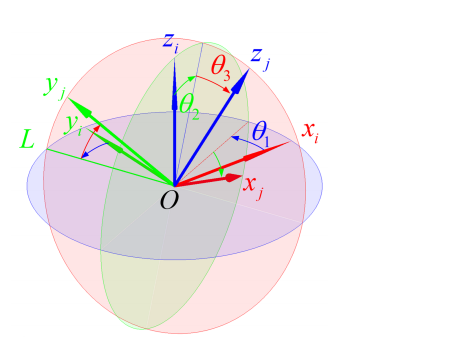
\includegraphics[width=0.8\textwidth]{Figure/PDF/SystemDynamicsModelingAndSimulation_75.png}
    \caption{体内ZYX转动（卡尔丹角）示意图}
    \label{fig:chapter7_euler_ZYX}
\end{figure}

从 $i$ 系到 $j$ 系的相对转动解读为绕连体坐标系（动系）坐标轴的三次相继转动，转轴分别为 $Z$、$Y$、$X$，转角分别为 $\theta_1$、$\theta_2$、$\theta_3$。

\begin{enumerate}
    \item $\theta_1$: 转轴 $z_i$，偏航角（$\psi$）
    \item $\theta_2$: 转轴 $L$，俯仰角（$\theta$）
    \item $\theta_3$: 转轴 $x_j$，滚转角（$\varphi$）
\end{enumerate}

坐标变换矩阵：
\begin{equation}
    \bm{A}_{ij} = \bm{A}_z(\theta_1)\bm{A}_y(\theta_2)\bm{A}_x(\theta_3).
\end{equation}

体内ZYX转动与坐标变换矩阵的关系\quad 由转角表示的坐标变换矩阵：
\begin{align}
    \bm{A}_{ij} &= \bm{A}_z(\theta_1)\bm{A}_y(\theta_2)\bm{A}_x(\theta_3)\notag\\
    &= \begin{bmatrix}
        \cos\theta_1 & -\sin\theta_1 & 0\\
        \sin\theta_1 & \cos\theta_1 & 0\\
        0 & 0 & 1
    \end{bmatrix}
    \begin{bmatrix}
        \cos\theta_2 & 0 & \sin\theta_2\\
        0 & 1 & 0\\
        -\sin\theta_2 & 0 & \cos\theta_2
    \end{bmatrix}
    \begin{bmatrix}
        1 & 0 & 0\\
        0 & \cos\theta_3 & -\sin\theta_3\\
        0 & \sin\theta_3 & \cos\theta_3
    \end{bmatrix}\notag\\
    &= \begin{bmatrix}
        c_1c_2 & -s_1c_3 + c_1s_2s_3 & s_1s_3 + c_1s_2c_3\\
        s_1c_2 & c_1c_3 + s_1s_2s_3 & -c_1s_3 + s_1s_2c_3\\
        -s_2 & c_2s_3 & c_2c_3
    \end{bmatrix}.
\end{align}

由坐标变换矩阵反求转角：
\begin{equation}
    \bm{A}_{ij} = \begin{bmatrix}
        c_1c_2 & -s_1c_3 + c_1s_2s_3 & s_1s_3 + c_1s_2c_3\\
        s_1c_2 & c_1c_3 + s_1s_2s_3 & -c_1s_3 + s_1s_2c_3\\
        -s_2 & c_2s_3 & c_2c_3
    \end{bmatrix}
    = \begin{bmatrix}
        a_{11} & a_{12} & a_{13}\\
        a_{21} & a_{22} & a_{23}\\
        a_{31} & a_{32} & a_{33}
    \end{bmatrix}.
\end{equation}

由上式可知，(I) 当 $s_2 = -a_{31} \approx 1$ 时，$c_2 \approx 0$，此时
\begin{equation}
    \bm{A}_{ij} = \begin{bmatrix}
        0 & -s_1c_3 + c_1s_3 & s_1s_3 + c_1c_3\\
        0 & c_1c_3 + s_1s_3 & -c_1s_3 + s_1c_3\\
        -1 & 0 & 0
    \end{bmatrix}
    = \begin{bmatrix}
        0 & a_{12} & a_{13}\\
        0 & a_{22} & a_{23}\\
        -1 & 0 & 0
    \end{bmatrix},
\end{equation}
\begin{equation}
    a_{23} = \sin(\theta_1 - \theta_3),\quad a_{22} = \cos(\theta_1 - \theta_3).
\end{equation}

可取
\begin{equation}
    \theta_2 = \pi/2 + 2k_1\pi,\quad \theta_1 - \theta_3 = \mathrm{atan2}(a_{23}, a_{22}) + 2k_2\pi.
\end{equation}

(II) 当 $s_2 = -a_{31} \approx -1$ 时，$c_2 \approx 0$，此时
\begin{equation}
    \bm{A}_{ij} = \begin{bmatrix}
        0 & -s_1c_3 - c_1s_3 & s_1s_3 - c_1c_3\\
        0 & c_1c_3 - s_1s_3 & -c_1s_3 - s_1c_3\\
        1 & 0 & 0
    \end{bmatrix}
    = \begin{bmatrix}
        0 & a_{12} & a_{13}\\
        0 & a_{22} & a_{23}\\
        1 & 0 & 0
    \end{bmatrix},
\end{equation}
\begin{equation}
    a_{23} = -\sin(\theta_1 + \theta_3),\quad a_{22} = \cos(\theta_1 + \theta_3).
\end{equation}

可取
\begin{equation}
    \theta_2 = -\pi/2 + 2k_1\pi,\quad \theta_1 + \theta_3 = \mathrm{atan2}(-a_{23}, a_{22}) + 2k_2\pi.
\end{equation}

(III) 当 $|s_2| = |a_{31}| \neq 1$ 时
\begin{equation}
    \begin{bmatrix}
        1 & -a_{31}\\
        -a_{31} & 1
    \end{bmatrix}
    \begin{bmatrix}
        c_1c_3\\
        s_1s_3
    \end{bmatrix}
    = \begin{bmatrix}
        a_{22}\\
        a_{13}
    \end{bmatrix}
    \Rightarrow \left\{\begin{aligned}
        c_1c_3 &= (a_{22} + a_{13}a_{31})/(1-a_{31}^2) =: b_1\\
        s_1s_3 &= (a_{13} + a_{22}a_{31})/(1-a_{31}^2) =: b_2
    \end{aligned}\right.
\end{equation}

\begin{equation}
    \begin{bmatrix}
        -a_{31} & -1\\
        -1 & -a_{31}
    \end{bmatrix}
    \begin{bmatrix}
        s_1c_3\\
        c_1s_3
    \end{bmatrix}
    = \begin{bmatrix}
        a_{23}\\
        a_{12}
    \end{bmatrix}
    \Rightarrow \left\{\begin{aligned}
        s_1c_3 &= (-a_{12} + a_{23}a_{31})/(1-a_{31}^2) =: b_3\\
        c_1s_3 &= (-a_{23} + a_{12}a_{31})/(1-a_{31}^2) =: b_4
    \end{aligned}\right.
\end{equation}

\begin{equation}
    \left\{\begin{aligned}
        \theta_1 + \theta_3 &= \mathrm{atan2}(b_3 + b_4,\, b_1 - b_2) =: b_5 + 2k_1\pi\\
        \theta_1 - \theta_3 &= \mathrm{atan2}(b_3 - b_4,\, b_1 + b_2) =: b_6 + 2k_2\pi
    \end{aligned}\right.
    \quad\Rightarrow\quad
    \left\{\begin{aligned}
        \theta_1 &= (b_5 + b_6)/2 + k_3\pi\\
        \theta_3 &= (b_5 - b_6)/2 - k_3\pi + 2k_4\pi
    \end{aligned}\right.
\end{equation}

体内ZYX转动与角速度投影列阵的关系\quad 由 $\tilde{\bm{\omega}}_{ij|j} = \bm{A}_{ij}^{\mathrm{T}}\dot{\bm{A}}_{ij}$ 可得：
\begin{equation}
    \bm{\omega}_{ij|j} = \begin{bmatrix}
        -\sin(\theta_2) & 0 & 1\\
        \cos(\theta_2)\sin(\theta_3) & \cos(\theta_3) & 0\\
        \cos(\theta_2)\cos(\theta_3) & -\sin(\theta_3) & 0
    \end{bmatrix}
    \begin{bmatrix}
        \dot{\theta}_1\\
        \dot{\theta}_2\\
        \dot{\theta}_3
    \end{bmatrix}
    =: \bm{H}_{\mathrm{BZYX}}\dot{\bm{\theta}}.
\end{equation}

系数矩阵的行列式为
\begin{equation}
    \det(\bm{H}_{\mathrm{BZYX}}) = -\cos(\theta_2),
\end{equation}

因此，当 $\theta_2 = \pi/2 + k\pi$ 时，不存在从 $\bm{\omega}_{ij|j}$ 到 $\dot{\bm{\theta}}$ 的对应关系；也不存在从 $\dot{\bm{\omega}}_{ij|j}$ 到 $\ddot{\bm{\theta}}$ 的对应关系。$\theta_2 = \pi/2 + k\pi$ 为此类三轴角的奇异点。

角速度列阵 $\bm{\omega}_{ij|j}$ 对体内ZYX转角 $\bm{\theta}$ 的偏导数满足
\begin{equation}
    \frac{\partial\bm{\omega}_{ij|j}}{\partial\bm{\theta}} = \begin{bmatrix}
        0 & -\cos(\theta_2)\dot{\theta}_1 & 0\\
        0 & -\sin(\theta_2)\sin(\theta_3)\dot{\theta}_1 & \cos(\theta_2)\cos(\theta_3)\dot{\theta}_1 - \sin(\theta_3)\dot{\theta}_2\\
        0 & -\sin(\theta_2)\cos(\theta_3)\dot{\theta}_1 & -\cos(\theta_2)\sin(\theta_3)\dot{\theta}_1 - \cos(\theta_3)\dot{\theta}_2
    \end{bmatrix}.
\end{equation}

%
% ---- 补充视角：Kane 书中的方向角体系 ----
\paragraph*{补充视角：方向角（空间三转角、体三转角、空间二转角、体二转角）（Kane《Spacecraft Dynamics》）}

以下补充 Kane 书中的方向角体系；前文体内 ZYX 转动属于体三转角（三个互异体轴）的特例，体内 ZXZ 转动属于体二转角（仅两个互异体轴）的特例，此处给出四种转角体系的统一公式、反解公式及其证明。


当刚体 $B$ 在参考系 $A$（也就是世界坐标系） 中作任意转动时，可以用三个角度 $\theta_1$、$\theta_2$、$\theta_3$ 来刻画其方向，这三个角度称为\textbf{方向角}。方向角可以通过依次进行三次简单转动得到，且这三次转动所绕的轴既可以取自固定在世界坐标系中的单位向量，也可以取自固定在刚体内部的单位向量。

\begin{figure}[H]
    \centering
    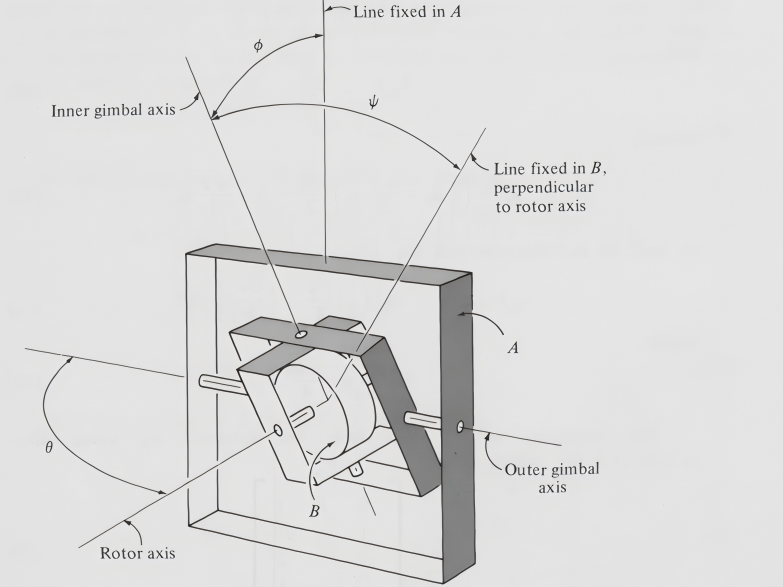
\includegraphics[width=0.8\textwidth]{Figure/陀螺转子.png}
        \caption{陀螺转子}
        \label{fig:陀螺转子}
\end{figure}

\blocksep

实现这一目标的第一种方法是依次对 $B$ 进行一次角度为 $\theta_1$ 的 $\mathbf{a}_1$ 旋转，一次角度为 $\theta_2$ 的 $\mathbf{a}_2$ 旋转，以及一次角度为 $\theta_3$ 的 $\mathbf{a}_3$ 旋转；在此过程中，$B$ 最终相对于 $A$ 的方向余弦矩阵为

\begin{equation}\label{eq:方向角:a1a2a3}
A = \left[
\begin{array}{ccc}
c_2 c_3 & s_1 s_2 c_3 - s_3 c_1 & c_1 s_2 c_3 + s_1 s_3 \\
c_2 s_3 & s_1 s_2 s_3 + c_1 c_3 & c_1 s_2 s_3 - s_1 c_3 \\
-s_2 & s_1 c_2 & c_1 c_2
\end{array}
\right]
\end{equation}

其中 $c_i \triangleq \cos\theta_i$，$s_i \triangleq \sin\theta_i$（$i=1,2,3$）。

若 $|a_{31}| \ne 1$，则通过取
$$
\theta_2 = \sin^{-1}(-a_{31}),\quad -\frac{\pi}{2} < \theta_2 < \frac{\pi}{2}
$$
可得到合适的 $\theta_1$、$\theta_2$、$\theta_3$ 值。接下来，在计算出 $c_2$ 后，定义 $\alpha$ 为
$$
\alpha \triangleq \sin^{-1}\frac{a_{32}}{c_2} \quad -\frac{\pi}{2} \le \alpha \le \frac{\pi}{2}
$$
并令
$$
\theta_1 = \begin{cases} \alpha & \text{如果 } a_{33} \ge 0 \\ \pi - \alpha & \text{如果 } a_{33} < 0 \end{cases}
$$
同样地，定义 $\beta$ 为
$$
\beta \triangleq \sin^{-1}\frac{a_{21}}{c_2} \quad -\frac{\pi}{2} \le \beta \le \frac{\pi}{2}
$$
并取
$$
\theta_3 = \begin{cases} \beta & \text{如果 } a_{11} \ge 0 \\ \pi - \beta & \text{如果 } a_{11} < 0 \end{cases}
$$

若 $|a_{31}| = 1$，则取
$$
\theta_2 = \begin{cases} -\dfrac{\pi}{2} & \text{如果 } a_{31} = 1 \\[4pt] \dfrac{\pi}{2} & \text{如果 } a_{31} = -1 \end{cases}
$$
并定义 $\alpha$ 为
$$
\alpha \triangleq \sin^{-1}(-a_{23}) \quad -\frac{\pi}{2} \le \alpha \le \frac{\pi}{2}
$$
并取
$$
\theta_1 = \begin{cases} \alpha & \text{如果 } a_{22} \ge 0 \\ \pi - \alpha & \text{如果 } a_{22} < 0 \end{cases}
$$
和
$$
\theta_3 = 0
$$
换句话说，这种情况下只需两次旋转即可。
\blocksep

实现相同目标的第二种方法是依次对 $B$ 进行一次角度为 $\theta_1$ 的 $\mathbf{b}_1$ 旋转，一次角度为 $\theta_2$ 的 $\mathbf{b}_2$ 旋转，以及一次角度为 $\theta_3$ 的 $\mathbf{b}_3$ 旋转。在上一次旋转之后，将 $\mathbf{a}_1$、$\mathbf{a}_2$、$\mathbf{a}_3$ 映射到 $\mathbf{b}_1$、$\mathbf{b}_2$、$\mathbf{b}_3$ 的矩阵 $A$ 如式~\eqref{eq:方向角:b1b2b3} 所示，则为

\begin{equation}\label{eq:方向角:b1b2b3}
A = \left[
\begin{array}{ccc}
c_2 c_3 & -c_2 s_3 & s_2 \\
s_1 s_2 c_3 + s_3 c_1 & -s_1 s_2 s_3 + c_3 c_1 & -s_1 c_2 \\
-c_1 s_2 c_3 + s_3 s_1 & c_1 s_2 s_3 + c_3 s_1 & c_1 c_2
\end{array}
\right]
\end{equation}

若 $|a_{13}| \ne 1$，则通过取
$$
\theta_2 = \sin^{-1} a_{13},\quad -\frac{\pi}{2} < \theta_2 < \frac{\pi}{2}
$$
可得到合适的 $\theta_1$、$\theta_2$、$\theta_3$ 值。此时定义
$$
\alpha \triangleq \sin^{-1}\frac{-a_{23}}{c_2} \quad -\frac{\pi}{2} \le \alpha \le \frac{\pi}{2}
$$
$$
\theta_1 = \begin{cases} \alpha & \text{如果 } a_{33} \ge 0 \\ \pi - \alpha & \text{如果 } a_{33} < 0 \end{cases}
$$
$$
\beta \triangleq \sin^{-1}\frac{-a_{12}}{c_2} \quad -\frac{\pi}{2} \le \beta \le \frac{\pi}{2}
$$
$$
\theta_3 = \begin{cases} \beta & \text{如果 } a_{11} \ge 0 \\ \pi - \beta & \text{如果 } a_{11} < 0 \end{cases}
$$

而如果 $|a_{13}| = 1$，则可以设
$$
\theta_2 = \begin{cases} \dfrac{\pi}{2} & \text{如果 } a_{13} = 1 \\[4pt] -\dfrac{\pi}{2} & \text{如果 } a_{13} = -1 \end{cases}
$$
$$
\alpha \triangleq \sin^{-1} a_{32} \quad -\frac{\pi}{2} \le \alpha \le \frac{\pi}{2}
$$
$$
\theta_1 = \begin{cases} \alpha & \text{如果 } a_{22} \ge 0 \\ \pi - \alpha & \text{如果 } a_{22} < 0 \end{cases}
$$
$$
\theta_3 = 0
$$
因此，再次仅需两次旋转即可。这两种方法将刚体 $B$ 转换为相对于参考系 $A$ 的期望方向的差异在于：第一种方法使用参考系中固定的单位向量，而第二种方法则使用刚体内部固定的单位向量。两种方法的共同点是，均使用了三个不同的单位向量。
\blocksep
此外，也可以通过进行三次连续旋转来将 $B$ 转换为相对于 $A$ 的任意方向，且这三次旋转仅涉及两个不同的单位向量，这些向量可以固定在参考系或刚体内部。具体而言，若刚体 $B$ 先依次经历一次 $\mathbf{a}_1$ 旋转角度为 $\theta_1$，再经历一次 $\mathbf{a}_2$ 旋转角度为 $\theta_2$，然后再次经历一次 $\mathbf{a}_1$ 旋转，但这次旋转角度为 $\theta_3$，则有

\begin{equation}\label{eq:方向角:a1a2a1}
A = \left[
\begin{array}{ccc}
c_2 & s_1 s_2 & c_1 s_2 \\
s_2 s_3 & c_1 c_3 - s_1 c_2 s_3 & -s_1 c_3 - c_1 c_2 s_3 \\
-s_2 c_3 & s_1 c_3 + c_1 c_2 s_3 & c_1 c_2 c_3 - s_1 s_3
\end{array}
\right]
\end{equation}

如果 $|a_{11}| \ne 1$，则可取
$$
\theta_2 = \cos^{-1} a_{11},\quad 0 < \theta_2 < \pi
$$
$$
\alpha \triangleq \sin^{-1}\frac{a_{12}}{s_2} \quad -\frac{\pi}{2} \le \alpha \le \frac{\pi}{2}
$$
$$
\theta_1 = \begin{cases} \alpha & \text{如果 } a_{13} \ge 0 \\ \pi - \alpha & \text{如果 } a_{13} < 0 \end{cases}
$$
$$
\beta \triangleq \sin^{-1}\frac{a_{21}}{s_2} \quad -\frac{\pi}{2} \le \beta \le \frac{\pi}{2}
$$
$$
\theta_3 = \begin{cases} \beta & \text{如果 } a_{31} < 0 \\ \pi - \beta & \text{如果 } a_{31} \ge 0 \end{cases}
$$

当 $|a_{11}| = 1$ 时，可以令
$$
\theta_2 = \begin{cases} 0 & \text{如果 } a_{11} = 1 \\ \pi & \text{如果 } a_{11} = -1 \end{cases}
$$
$$
\alpha \triangleq \sin^{-1}(-a_{23}) \quad -\frac{\pi}{2} \le \alpha \le \frac{\pi}{2}
$$
$$
\theta_1 = \begin{cases} \alpha & \text{如果 } a_{22} \ge 0 \\ \pi - \alpha & \text{如果 } a_{22} < 0 \end{cases}
$$
$$
\theta_3 = 0
$$

最后，如果连续的旋转依次为：先以 $\mathbf{b}_1$ 旋转角度 $\theta_1$，再以 $\mathbf{b}_2$ 旋转角度 $\theta_2$，然后再次以 $\mathbf{b}_1$ 旋转，但这次旋转角度为 $\theta_3$，则

\begin{equation}\label{eq:方向角:b1b2b1}
A = \left[
\begin{array}{ccc}
c_2 & s_2 s_3 & s_2 c_3 \\
s_1 s_2 & -s_1 c_2 s_3 + c_3 c_1 & -s_1 c_2 c_3 - s_3 c_1 \\
-c_1 s_2 & c_1 c_2 s_3 + c_3 s_1 & c_1 c_2 c_3 - s_3 s_1
\end{array}
\right]
\end{equation}

如果 $|a_{11}| \ne 1$，则可以通过以下方式求出 $\theta_1$、$\theta_2$ 和 $\theta_3$
$$
\theta_2 = \cos^{-1} a_{11} \quad 0 < \theta_2 < \pi
$$
$$
\alpha \triangleq \sin^{-1} \frac{a_{21}}{s_2} \quad -\frac{\pi}{2} \le \alpha \le \frac{\pi}{2}
$$
$$
\theta_1 = \begin{cases} \alpha & \text{如果 } a_{31} < 0 \\ \pi - \alpha & \text{如果 } a_{31} \ge 0 \end{cases}
$$
$$
\beta \triangleq \sin^{-1}\frac{a_{12}}{s_2} \quad -\frac{\pi}{2} \le \beta \le \frac{\pi}{2}
$$
$$
\theta_3 = \begin{cases} \beta & \text{如果 } a_{13} \ge 0 \\ \pi - \beta & \text{如果 }a_{13} < 0 \end{cases}
$$

而当 $|a_{11}| = 1$ 时，可使用
$$
\theta_2 = \begin{cases} 0 & \text{如果 } a_{11} = 1 \\ \pi & \text{如果 } a_{11} = -1 \end{cases}
$$
$$
\alpha \triangleq \sin^{-1} a_{32} \quad -\frac{\pi}{2} \le \alpha \le \frac{\pi}{2}
$$
$$
\theta_1 = \begin{cases} \alpha & \text{如果 } a_{13} \ge 0 \\ \pi - \alpha & \text{如果 } a_{13} < 0 \end{cases}
$$
$$
\theta_3 = 0
$$


式~\eqref{eq:方向角:a1a2a3} 与式~\eqref{eq:方向角:b1b2b3} 中的矩阵彼此紧密相关：将其中一个矩阵中的 $\theta_i$ 替换为 $-\theta_i$（$i=1,2,3$）并转置，即可得到另一个；式~\eqref{eq:方向角:a1a2a1} 与式~\eqref{eq:方向角:b1b2b1} 中的矩阵也具有类似关系。这一事实具有如下物理意义（可借助方向余弦矩阵的正交性 $\bm{A}^{-1}=\bm{A}^{\mathrm{T}}$ 加以验证）：若刚体 $B$ 先后经历转角分别为 $\theta_1$、$\theta_2$、$\theta_3$ 的 $\mathbf{a}_1$、$\mathbf{a}_2$、$\mathbf{a}_3$ 旋转，那么接下来再使 $B$ 先后经历转角分别为 $\theta_1$、$\theta_2$、$\theta_3$ 的 $-\mathbf{b}_1$、$-\mathbf{b}_2$、$-\mathbf{b}_3$ 旋转，即可使 $B$ 恢复到它在 $A$ 中的初始方向。
\blocksep
类似地，仅使用四个单位向量，即可使 $B$ 依次经历以 $\theta_1\mathbf{a}_1,\theta_2\mathbf{a}_2,\theta_3\mathbf{a}_1,-\theta_1\mathbf{b}_1,-\theta_2\mathbf{b}_2,-\theta_3\mathbf{b}_1$ 表征的连续旋转，而不使 $B$ 在 $A$ 中的方向产生任何净变化。此外，涉及固定在 $A$ 中的单位向量的那些旋转，无论发生在涉及固定在 $B$ 中的单位向量的那些旋转之前还是之后，结果都一样；也就是说，由 $\theta_1\mathbf{b}_1,\theta_2\mathbf{b}_2,\theta_3\mathbf{b}_3,-\theta_1\mathbf{a}_1,-\theta_2\mathbf{a}_2,-\theta_3\mathbf{a}_3$ 以及由 $\theta_1\mathbf{b}_1,\theta_2\mathbf{b}_2,\theta_3\mathbf{b}_1,-\theta_1\mathbf{a}_1,-\theta_2\mathbf{a}_2,-\theta_3\mathbf{a}_1$ 表示的连续旋转序列，对 $B$ 在 $A$ 中的方向同样不产生净效果。

为了指明所用的是哪一组三个角度，可以称第一种方法（式~\eqref{eq:方向角:a1a2a3} 及其反解公式）对应的为\textbf{空间三角度}（space-three angles），第二种方法（式~\eqref{eq:方向角:b1b2b3} 及其反解公式）对应的为\textbf{体三角度}（body-three angles），第三种方法（式~\eqref{eq:方向角:a1a2a1} 及其反解公式）对应的为\textbf{空间二角度}（space-two angles），第四种方法（式~\eqref{eq:方向角:b1b2b1} 及其反解公式）对应的为\textbf{体二角度}（body-two angles）；即使所用的角度与单位向量采用了上述各式以外的符号表示，这一术语仍然有意义。

现代工程中，这些方向角已有更常用的名称。航空航天与机器人学中最常用的\textbf{横滚—俯仰—偏航角}（roll--pitch--yaw angles，又称 Tait--Bryan 角或 Cardan 角）依次绕刚体内部的 $z$、$y$、$x$ 轴转动偏航角 $\psi$、俯仰角 $\theta$、横滚角 $\phi$，属于\textbf{体三角度}；当取 $\mathbf{b}_1=\mathbf{x}$、$\mathbf{b}_2=\mathbf{y}$、$\mathbf{b}_3=\mathbf{z}$ 且 $(\theta_1,\theta_2,\theta_3)=(\phi,\theta,\psi)$ 时，式~\eqref{eq:方向角:b1b2b3} 恰给出其旋转矩阵
$$
R(\phi,\theta,\psi)=R_x(\phi)\,R_y(\theta)\,R_z(\psi)
=\left[
\begin{array}{ccc}
c_\theta c_\psi & -c_\theta s_\psi & s_\theta\\
s_\phi s_\theta c_\psi+c_\phi s_\psi & -s_\phi s_\theta s_\psi+c_\phi c_\psi & -s_\phi c_\theta\\
-c_\phi s_\theta c_\psi+s_\phi s_\psi & c_\phi s_\theta s_\psi+s_\phi c_\psi & c_\phi c_\theta
\end{array}
\right].
$$
\textbf{经典欧拉角}（classical Euler angles，进动—章动—自转）则采用 $z$--$x$--$z$ 转序，依次绕体 $z$ 轴转动进动角 $\psi$、绕体 $x$ 轴转动章动角 $\theta$、再绕体 $z$ 轴转动自转角 $\phi$，属于\textbf{体二角度}，其旋转矩阵为
$$
R(\phi,\theta,\psi)=R_z(\phi)\,R_x(\theta)\,R_z(\psi)
=\left[
\begin{array}{ccc}
c_\phi c_\psi-s_\phi c_\theta s_\psi & -c_\phi s_\psi-s_\phi c_\theta c_\psi & s_\phi s_\theta\\
s_\phi c_\psi+c_\phi c_\theta s_\psi & -s_\phi s_\psi+c_\phi c_\theta c_\psi & -c_\phi s_\theta\\
s_\theta s_\psi & s_\theta c_\psi & c_\theta
\end{array}
\right].
$$
其中 $c_\alpha\triangleq\cos\alpha$、$s_\alpha\triangleq\sin\alpha$；$R_x(\alpha),R_y(\alpha),R_z(\alpha)$ 分别表示绕刚体内部 $x$、$y$、$z$ 轴转动角 $\alpha$ 的基元旋转矩阵。至于\textbf{空间三角度}与\textbf{空间二角度}，则对应\textbf{外旋欧拉角}（extrinsic Euler angles），即转轴固定于参考系 $A$ 中的转序。

此外，一旦以这种方式确定了三个角度，总可以直接利用这些方程找到式~\eqref{eq:方向角:a1a2a3}、\eqref{eq:方向角:b1b2b3}、\eqref{eq:方向角:a1a2a1} 或 \eqref{eq:方向角:b1b2b1} 的适当替代。例如，设 $\mathbf{x},\mathbf{y},\mathbf{z}$ 与 $\bm{\xi},\bm{\eta},\bm{\zeta}$ 分别为固定在参考系 $A$ 与刚体 $B$ 中的两组成右手正交单位向量，且初始时 $\mathbf{x}=\bm{\xi}$、$\mathbf{y}=\bm{\eta}$、$\mathbf{z}=\bm{\zeta}$；设 $B$ 依次经历角度为 $\gamma$ 的 $\mathbf{z}$ 旋转、角度为 $\beta$ 的 $\mathbf{y}$ 旋转和角度为 $\alpha$ 的 $\mathbf{x}$ 旋转；要求确定矩阵 $L$ 的各元素 $L_{ij}$（$i,j=1,2,3$），使得在最后一次旋转之后满足
$$
[\bm{\xi}\ \ \bm{\eta}\ \ \bm{\zeta}]=[\mathbf{x}\ \ \mathbf{y}\ \ \mathbf{z}]L
$$
于是，把 $\alpha$、$\beta$、$\gamma$ 认作空间三角度，可引入 $\mathbf{a}_i$、$\mathbf{b}_i$ 与 $\theta_i$（$i=1,2,3$）如下：
$$
\mathbf{a}_1\triangleq\mathbf{z},\qquad \mathbf{a}_2\triangleq\mathbf{y},\qquad \mathbf{a}_3\triangleq-\mathbf{x}
$$
$$
\mathbf{b}_1\triangleq\bm{\zeta},\qquad \mathbf{b}_2\triangleq\bm{\eta},\qquad \mathbf{b}_3\triangleq-\bm{\xi}
$$
$$
\theta_1\triangleq\gamma,\qquad \theta_2\triangleq\beta,\qquad \theta_3\triangleq-\alpha
$$
此时给定的旋转序列由 $\theta_1\mathbf{a}_1,\theta_2\mathbf{a}_2,\theta_3\mathbf{a}_3$ 表示；然后参照式~\eqref{eq:方向角:a1a2a3}，即可用 $\alpha$、$\beta$、$\gamma$ 表示与 $L_{ij}$ 相关的内积。例如，
$$
L_{21}=\mathbf{y}\cdot\bm{\xi}=\mathbf{a}_2\cdot(-\mathbf{b}_3)=-a_{23}=-c_1s_2s_3+c_3s_1=\cos\gamma\sin\beta\sin\alpha+\cos\alpha\sin\gamma
$$
\begin{proof}
    为验证式~\eqref{eq:方向角:a1a2a3} 的正确性，可运用式~\eqref{eq:连续转动:方向余弦乘积}，并借助式~\eqref{eq:方向余弦矩阵计算式紧凑} 与式~\eqref{eq:方向余弦矩阵计算式} 构造 $\bm{C}_{A\bar B}$、$C_{\bar B\bar B}$ 与 $\bm{C}_{\bar B B}$。具体而言，对 $\mathbf{a}_1$ 旋转，令
$$
\bm{C}_{A\bar B}=\begin{bmatrix}1&0&0\\0&c_1&-s_1\\0&s_1&c_1\end{bmatrix}
$$
其次，为构造刻画 $\mathbf{a}_2$ 旋转的矩阵 $C_{\bar B\bar B}$，令 $\bm{\lambda}_A$ 与 $\bm{\lambda}_{\bar B}$ 分别表示以 $\mathbf{a}_2\cdot\mathbf{a}_i$ 与 $\mathbf{a}_2\cdot\mathbf{b}_i$（$i=1,2,3$）为元素的行矩阵，则
$$
\bm{\lambda}_A=[0\ \ 1\ \ 0]
$$
$$
\bm{\lambda}_{\bar B}=\bm{\lambda}_A\,\bm{C}_{A\bar B}=[0\ \ c_1\ \ -s_1]
$$
于是由式~\eqref{eq:方向余弦矩阵计算式}，令 $\lambda_1=0$、$\lambda_2=c_1$、$\lambda_3=-s_1$、$\theta=\theta_2$，得
$$
C_{\bar B\bar B}=\begin{bmatrix}c_2&s_1s_2&c_1s_2\\-s_1s_2&1+s_1^2(c_2-1)&s_1c_1(c_2-1)\\-c_1s_2&s_1c_1(c_2-1)&1+c_1^2(c_2-1)\end{bmatrix}
$$
与头两次旋转等价的单次旋转所对应的矩阵 $\bm{C}_{A\bar B}$ 为
$$
\bm{C}_{A\bar B}=\bm{C}_{A\bar B}\,C_{\bar B\bar B}=\begin{bmatrix}c_2&s_1s_2&c_1s_2\\0&c_1&-s_1\\-s_2&s_1c_2&c_1c_2\end{bmatrix}
$$
为把 $\mathbf{a}_3$ 分解为构造矩阵 $\bm{C}_{\bar B B}$ 所需的分量，可借助式~\eqref{eq:方向余弦的定义} 得到
$$
[0\ \ 0\ \ 1]\,\bm{C}_{A\bar B}=[-s_2\ \ s_1c_2\ \ c_1c_2]
$$
之后由式~\eqref{eq:方向余弦矩阵计算式} 得
$$
\bm{C}_{\bar B B}=\begin{bmatrix}s_2^2+c_2^2c_3&-c_2[c_1s_3+s_1s_2(1-c_3)]&c_2[s_1s_3-c_1s_2(1-c_3)]\\c_2[c_1s_3+s_1s_2(1-c_3)]&c_3(1-s_1^2c_2^2)+s_1^2c_2^2&s_2s_3+s_1c_1c_2^2(1-c_3)\\-c_2[s_1s_3+c_1s_2(1-c_3)]&-s_2s_3+s_1c_1c_2^2(1-c_3)&1-(s_2^2+s_1^2c_2^2)(1-c_3)\end{bmatrix}
$$
将上面得到的 $\bm{C}_{A\bar B}$、$C_{\bar B\bar B}$ 与 $\bm{C}_{\bar B B}$ 三个矩阵代入式~\eqref{eq:连续转动:方向余弦乘积}，即可直接得到式~\eqref{eq:方向角:a1a2a3}。

式~\eqref{eq:方向角:b1b2b3} 可由式~\eqref{eq:连续转动:方向余弦乘积} 配以下面三个矩阵得到：
$$
\bm{C}_{A\bar B}=\begin{bmatrix}1&0&0\\0&c_1&-s_1\\0&s_1&c_1\end{bmatrix}
$$
$$
C_{\bar B\bar B}=\begin{bmatrix}c_2&0&s_2\\0&1&0\\-s_2&0&c_2\end{bmatrix}
$$
$$
\bm{C}_{\bar B B}=\begin{bmatrix}c_3&-s_3&0\\s_3&c_3&0\\0&0&1\end{bmatrix}
$$

第一种方法的反解公式与第二种方法的反解公式分别是式~\eqref{eq:方向角:a1a2a3} 与式~\eqref{eq:方向角:b1b2b3} 的直接推论；而第三、第四种方法（式~\eqref{eq:方向角:a1a2a1} 与式~\eqref{eq:方向角:b1b2b1} 及其反解公式）可由与前两种方法推导类似的方法得到。

\end{proof}

%=============================================================
\section{坐标系姿态广义坐标的其他形式}
%=============================================================

\begin{enumerate}
    \item 旋转向量/罗德里格斯向量
    \begin{equation}
        \bm{\rho} = \theta\bm{n}.
    \end{equation}

    \item 罗德里格斯参数/吉布斯向量（Rodrigues parameters / Gibbs vector）
    \begin{equation}
        \bm{g} = \bm{n}\tan\frac{\theta}{2}.
    \end{equation}

    \item 修正的罗德里格斯参数（Modified Rodrigues Parameters, MRP）
    \begin{equation}
        \bm{\sigma} = \bm{n}\tan\frac{\theta}{4}.
    \end{equation}
\end{enumerate}
%
% ---- 补充视角：Kane 书中的罗德里格斯参数 ----
\paragraph*{补充视角：罗德里格斯参数（Kane《Spacecraft Dynamics》）}

以下补充 Kane 书中的罗德里格斯参数 $\bm{\rho}=\bm{\lambda}\tan(\theta/2)$，其与上列“罗德里格斯参数/吉布斯向量”$\bm{g}$ 是同一组参数的不同记法。

罗德里格斯参数（Rodrigues Parameters），也叫罗德里格斯向量，但是使用的比较少。虽然目的是少用一个参数，但是引入了奇异点，且物理意义不明，所以在实际应用中，很少使用。引入定义，不多赘述。
\begin{mydefinition}{罗德里格斯参数}
    设$\bm{\lambda}$为转轴单位向量，$\theta$为转角，则罗德里格斯参数定义为：
    \begin{equation}
        \label{eq:罗德里格斯参数定义}
        \begin{aligned}
            &\bm{\rho} \triangleq \bm{\lambda}\tan \frac{\theta}{2}\\
            &\rho_i \triangleq \bm{\rho} \cdot \bm{a}_i=\bm{\rho} \cdot \bm{b}_i\quad(i=1,2,3)
        \end{aligned}
    \end{equation}
\end{mydefinition}
在旋转前，有 $\mathbf{a}_i = \mathbf{b}_i$（$i = 1, 2, 3$）。（当讨论涉及两个以上物体或参考系时，将使用如 $\bm{\rho}_{AB}$ 和 $\rho_{AB,i}$ 等符号。）

罗德里格斯参数与欧拉参数密切相关（见第~\ref{sec:euler-parameters}~节）：
$$\rho_i = \frac{\epsilon_i}{\epsilon_4} \quad (i = 1, 2, 3)$$

罗德里格斯参数相较于欧拉参数的优势在于其数量更少；但这一优势有时会被抵消，因为罗德里格斯参数可能取到无穷大，而任何欧拉参数的绝对值均不能超过1。

用罗德里格斯参数表示时，方向余弦矩阵 $\bm{A}$（见第 3.1 节）的形式为
$$
\bm{A} = \frac{1}{1 + \rho_1^2 + \rho_2^2 + \rho_3^2}
\begin{bmatrix}
1 + \rho_1^2 - \rho_2^2 - \rho_3^2 & 2(\rho_1 \rho_2 - \rho_3) & 2(\rho_3 \rho_1 + \rho_2) \\
2(\rho_1 \rho_2 + \rho_3) & 1 + \rho_2^2 - \rho_3^2 - \rho_1^2 & 2(\rho_2 \rho_3 - \rho_1) \\
2(\rho_3 \rho_1 - \rho_2) & 2(\rho_2 \rho_3 + \rho_1) & 1 + \rho_3^2 - \rho_1^2 - \rho_2^2
\end{bmatrix}
$$
罗德里格斯向量可用于建立第~\ref{sec:simple-rotation}~节中定义的向量 $\mathbf{a}$ 和 $\mathbf{b}$ 的差与和之间的简单关系：
\begin{equation}
    \label{eq:罗德里格斯向量表示的和差关系}
    \mathbf{a} - \mathbf{b} = (\mathbf{a} + \mathbf{b}) \times \bm{\rho}
\end{equation}

该关系在多种推导中非常有用，例如用于证明以下表达式是罗德里格斯向量的表示形式，该向量可用来实现A与B之间相对方向的指定变化：
$$\bm{\rho} = \frac{(\bm{\alpha}_1 - \bm{\beta}_1) \times (\bm{\alpha}_2 - \bm{\beta}_2)}{(\bm{\alpha}_1 + \bm{\beta}_1) \cdot (\bm{\alpha}_2 - \bm{\beta}_2)}$$
其中，$\bm{\alpha}_i$ 和 $\bm{\beta}_i$（$i = 1, 2$）分别固定于A和B中，在相对方向发生变化前满足 $\bm{\alpha}_i = \bm{\beta}_i$（$i = 1, 2$）。对于此类旋转的罗德里格斯参数可表示为
$$\rho_1 = \frac{a_{32} - a_{23}}{1 + a_{11} + a_{22} + a_{33}}, \qquad \rho_2 = \frac{a_{13} - a_{31}}{1 + a_{11} + a_{22} + a_{33}}, \qquad \rho_3 = \frac{a_{21} - a_{12}}{1 + a_{11} + a_{22} + a_{33}}$$
% 注：$\rho_2$、$\rho_3$ 原转写缺失，已按 Rodrigues 参数的循环对称关系补全，请对照原书核对。
%=============================================================
\section{相继转动}
%=============================================================

\textbf{方向余弦矩阵与转轴转角的关系}\quad 用转轴和转角表示的方向余弦矩阵：
\begin{equation}
    \bm{A}_{ij} = \bm{I}_3\cos\theta + \tilde{\bm{n}}\sin\theta + \bm{n}\bm{n}^{\mathrm{T}}(1-\cos\theta).
\end{equation}

当转轴 $\tilde{\bm{n}}$ 相对于 $i$ 系和 $j$ 系固定时，
\begin{equation}
    \dot{\bm{A}}_{ij} = (-\bm{I}_3\sin\theta + \tilde{\bm{n}}\cos\theta + \bm{n}\bm{n}^{\mathrm{T}}\sin\theta)\,\dot{\theta}.
\end{equation}

接下来对
\begin{align}
    \tilde{\bm{\omega}}_{ij|j} &= \bm{A}_{ij}^{\mathrm{T}}\dot{\bm{A}}_{ij}\notag\\
    &= \left[\bm{I}_3\cos\theta + \tilde{\bm{n}}^{\mathrm{T}}\sin\theta + \bm{n}\bm{n}^{\mathrm{T}}(1-\cos\theta)\right](-\bm{I}_3\sin\theta + \tilde{\bm{n}}\cos\theta + \bm{n}\bm{n}^{\mathrm{T}}\sin\theta)\,\dot{\theta}
\end{align}

进行化简。

角速度矢量列阵的叉乘矩阵（$\tilde{\bm{n}}\tilde{\bm{n}} = \bm{n}\bm{n}^{\mathrm{T}} - \bm{I}_3$）：
\begin{align}
    \tilde{\bm{\omega}}_{ij|j} &= \bm{A}_{ij}^{\mathrm{T}}\dot{\bm{A}}_{ij}\notag\\
    &= \left[\bm{I}_3\cos\theta + \tilde{\bm{n}}^{\mathrm{T}}\sin\theta + \bm{n}\bm{n}^{\mathrm{T}}(1-\cos\theta)\right](-\bm{I}_3\sin\theta + \tilde{\bm{n}}\cos\theta + \bm{n}\bm{n}^{\mathrm{T}}\sin\theta)\,\dot{\theta}\notag\\
    &= (-\bm{I}_3\sin\theta\cos\theta + \tilde{\bm{n}}\cos^2\theta + \bm{n}\bm{n}^{\mathrm{T}}\sin\theta\cos\theta)\,\dot{\theta}\notag\\
    &\quad + \left(-\tilde{\bm{n}}^{\mathrm{T}}\sin^2\theta + \tilde{\bm{n}}^{\mathrm{T}}\tilde{\bm{n}}\sin\theta\cos\theta + \tilde{\bm{n}}^{\mathrm{T}}\bm{n}\bm{n}^{\mathrm{T}}\sin^2\theta\right)\dot{\theta}\notag\\
    &\quad + \left[-\bm{n}\bm{n}^{\mathrm{T}}\sin\theta(1-\cos\theta) + \bm{n}\bm{n}^{\mathrm{T}}\tilde{\bm{n}}\cos\theta(1-\cos\theta) + \bm{n}\bm{n}^{\mathrm{T}}\bm{n}\bm{n}^{\mathrm{T}}\sin\theta(1-\cos\theta)\right]\dot{\theta}\notag\\
    &= \tilde{\bm{n}}(\cos^2\theta + \sin^2\theta)\dot{\theta}\notag\\
    &\quad + \left[-\bm{I}_3 + \bm{n}\bm{n}^{\mathrm{T}} - (\bm{n}\bm{n}^{\mathrm{T}} - \bm{I}_3)\right]\sin\theta\cos\theta\dot{\theta}\notag\\
    &= \tilde{\bm{n}}\dot{\theta}\notag\\
    &= \widetilde{\bm{n}\dot{\theta}}.
\end{align}

由此可知
\begin{equation}
    \bm{\omega}_{ij|j} = \bm{n}\dot{\theta}.
\end{equation}

当转轴 $\tilde{\bm{n}}$ 相对于 $i$ 系和 $j$ 系固定时
\begin{equation}
    \bm{\omega}_{ij|j} = \bm{n}\dot{\theta}.
\end{equation}

此时
\begin{align}
    \bm{\omega}_{ij}^i &= \bm{A}_{ij}\bm{\omega}_{ij|j}\notag\\
    &= \left[\bm{I}_3\cos\theta + \tilde{\bm{n}}\sin\theta + \bm{n}\bm{n}^{\mathrm{T}}(1-\cos\theta)\right]\bm{n}\dot{\theta}\notag\\
    &= \bm{n}\dot{\theta} = \bm{\omega}_{ij|j}.
\end{align}

当涉及多次相对转动时，为避免歧义，以上两式又可记为
\begin{equation}
    \bm{\omega}_{ij}^i = \bm{\omega}_{ij|j} = \bm{n}_{ij}\dot{\theta}_{ij}.
\end{equation}

设 $l$ 系由 $i$ 系经三次相继转动获得，相应的方向余弦矩阵表示为
\begin{equation}
    \bm{A}_{il} = \bm{A}_{ij}(\bm{n}_{ij}, \theta_{ij})\bm{A}_{jk}(\bm{n}_{jk}, \theta_{jk})\bm{A}_{kl}(\bm{n}_{kl}, \theta_{kl}),
\end{equation}

且 $\bm{n}_{ij}$，$\bm{n}_{jk}$，$\bm{n}_{kl}$ 不随时间变化。此时，上式对时间的一阶导数可表示为
\begin{equation}
    \bm{A}_{il}\tilde{\bm{\omega}}_{il|l} = \bm{A}_{ij}\tilde{\bm{\omega}}_{ij|j}\bm{A}_{jk}\bm{A}_{kl} + \bm{A}_{ij}\bm{A}_{jk}\tilde{\bm{\omega}}_{jk|k}\bm{A}_{kl} + \bm{A}_{ij}\bm{A}_{jk}\bm{A}_{kl}\tilde{\bm{\omega}}_{kl|l},
\end{equation}

式中
\begin{equation}
    \bm{\omega}_{ij|j} = \bm{n}_{ij}\dot{\theta}_{ij},\quad \bm{\omega}_{jk|k} = \bm{n}_{jk}\dot{\theta}_{jk},\quad \bm{\omega}_{kl|l} = \bm{n}_{kl}\dot{\theta}_{kl}.
\end{equation}

则
\begin{equation}
    \bm{\omega}_{il|l} = \bm{A}_{jl}^{\mathrm{T}}\bm{\omega}_{ij|j} + \bm{A}_{kl}^{\mathrm{T}}\bm{\omega}_{jk|k} + \bm{\omega}_{kl|l} = \bm{A}_{jl}^{\mathrm{T}}\bm{n}_{ij}\dot{\theta}_{ij} + \bm{A}_{kl}^{\mathrm{T}}\bm{n}_{jk}\dot{\theta}_{jk} + \bm{n}_{kl}\dot{\theta}_{kl}.
\end{equation}
%
% ---- 补充视角：Kane 书中的连续转动合成 ----
\paragraph*{补充视角：连续转动的合成公式及其证明（Kane《Spacecraft Dynamics》）}

前文给出了固定转轴情形下相继转动的角速度合成；以下补充一般情形下用方向余弦矩阵、罗德里格斯向量与欧拉参数刻画的连续转动合成公式及其证明。


当刚体 $B$ 在参考系 $A$ 中进行两次连续简单转动时，每一次转动以及与之等价的单次转动都可以用方向余弦、欧拉参数和罗德里格斯参数描述；无论采用哪种描述方式，与各次转动相关的量都可以与刻画单次等效转动的量联系起来。在讨论这些关系时，引入一个虚拟刚体 $\overline{B}$ 会有所帮助：它在 $B$ 进行第一次转动时与 $B$ 同步运动，而在 $B$ 进行第二次转动时保持与 $A$ 固结。在分析上，第一次转动可视为 $\overline{B}$ 相对于 $A$ 的转动，第二次转动则视为 $B$ 相对于 $\overline{B}$ 的转动。

若 $\mathbf{a}_i\,(i=1,2,3)$、$\mathbf{b}_i\,(i=1,2,3)$、$\overline{\mathbf{b}}_i\,(i=1,2,3)$ 分别为固定在 $A$、$B$、$\overline{B}$ 中的三组成右手正交单位向量，且在 $B$ 在 $A$ 中作第一次转动之前有 $\mathbf{a}_i=\mathbf{b}_i=\overline{\mathbf{b}}_i\,(i=1,2,3)$；若 $\bm{C}_{A\bar B}$、$\bm{C}_{\bar B B}$、$\bm{C}_{AB}$ 分别为刻画第一次、第二次和单次等效转动的方向余弦矩阵，使得

\begin{equation}\label{eq:连续转动:C_Abar_B}
\begin{bmatrix}\overline{\mathbf{b}}_1 & \overline{\mathbf{b}}_2 & \overline{\mathbf{b}}_3\end{bmatrix}
=\begin{bmatrix}\mathbf{a}_1 & \mathbf{a}_2 & \mathbf{a}_3\end{bmatrix}\,\bm{C}_{A\bar B}
\end{equation}
\begin{equation}\label{eq:连续转动:C_Bar_B_B}
\begin{bmatrix}\mathbf{b}_1 & \mathbf{b}_2 & \mathbf{b}_3\end{bmatrix}
=\begin{bmatrix}\overline{\mathbf{b}}_1 & \overline{\mathbf{b}}_2 & \overline{\mathbf{b}}_3\end{bmatrix}\,\bm{C}_{\bar B B}
\end{equation}
\begin{equation}\label{eq:连续转动:C_AB}
\begin{bmatrix}\mathbf{b}_1 & \mathbf{b}_2 & \mathbf{b}_3\end{bmatrix}
=\begin{bmatrix}\mathbf{a}_1 & \mathbf{a}_2 & \mathbf{a}_3\end{bmatrix}\,\bm{C}_{AB}
\end{equation}

则 $\bm{C}_{AB}$（用 $\bm{C}_{A\bar B}$ 和 $\bm{C}_{\bar B B}$ 表达）由下式给出

\begin{equation}\label{eq:连续转动:方向余弦乘积}
\bm{C}_{AB}=\bm{C}_{A\bar B}\,\bm{C}_{\bar B B}
\end{equation}

类似地，对罗德里格斯向量有

\begin{equation}\label{eq:连续转动:罗德里格斯乘积}
\bm{\rho}_{AB}=\frac{\bm{\rho}_{A\bar B}+\bm{\rho}_{\bar B B}+\bm{\rho}_{\bar B B}\times\bm{\rho}_{A\bar B}}{1-\bm{\rho}_{A\bar B}\cdot\,\bm{\rho}_{\bar B B}}
\end{equation}
利用叉乘矩阵 $\bm{\rho}_{\bar B B}\times\bm{\rho}_{A\bar B}=\tilde{\bm{\rho}}_{\bar B B}\,\bm{\rho}_{A\bar B}$，上式可写成
\begin{equation}
\bm{\rho}_{AB}=\frac{\bm{\rho}_{A\bar B}+\bm{\rho}_{\bar B B}+\tilde{\bm{\rho}}_{\bar B B}\,\bm{\rho}_{A\bar B}}{1-\bm{\rho}_{A\bar B}^{\mathrm{T}}\bm{\rho}_{\bar B B}}.
\label{eq:连续转动:罗德里格斯乘积矩阵}
\end{equation}

要给出欧拉参数下的相应关系，首先定义三组欧拉参数：设 $\mathbf{b}_i$、$\overline{\mathbf{b}}_i\,(i=1,2,3)$ 在第二次转动后取所示方向；并设 $\theta_1$、$\theta_2$、$\theta$ 分别为第一次、第二次和等效转动的弧度

\begin{equation}\label{eq:连续转动:epsilon_Abar_B_i}
\epsilon_{A\bar B,i}\triangleq\,\bm{\epsilon}_{A\bar B}\cdot\mathbf{a}_i=\bm{\epsilon}_{A\bar B}\cdot\overline{\mathbf{b}}_i\quad(i=1,2,3)
\end{equation}
\begin{equation}\label{eq:连续转动:epsilon_Bar_B_B_i}
\epsilon_{\bar B B,i}\triangleq\,\bm{\epsilon}_{\bar B B}\cdot\overline{\mathbf{b}}_i=\bm{\epsilon}_{\bar B B}\cdot\mathbf{b}_i\quad(i=1,2,3)
\end{equation}
\begin{equation}\label{eq:连续转动:epsilon_AB_i}
\epsilon_{AB,i}\triangleq\,\bm{\epsilon}_{AB}\cdot\mathbf{a}_i=\bm{\epsilon}_{AB}\cdot\mathbf{b}_i\quad(i=1,2,3)
\end{equation}
$$
\epsilon_{A\bar B,4}\triangleq\cos\frac{\theta_1}{2},\qquad
\epsilon_{\bar B B,4}\triangleq\cos\frac{\theta_2}{2},\qquad
\epsilon_{AB,4}\triangleq\cos\frac{\theta}{2}
$$

于是可得
\begin{equation}\label{eq:连续转动:欧拉参数关系}
\begin{bmatrix}
\epsilon_{AB,1}\\[2pt] \epsilon_{AB,2}\\[2pt] \epsilon_{AB,3}\\[2pt] \epsilon_{AB,4}
\end{bmatrix}
=
\begin{bmatrix}
\epsilon_{A\bar B,4} & -\epsilon_{A\bar B,3} & \epsilon_{A\bar B,2} & \epsilon_{A\bar B,1}\\
\epsilon_{A\bar B,3} & \epsilon_{A\bar B,4} & -\epsilon_{A\bar B,1} & \epsilon_{A\bar B,2}\\
-\epsilon_{A\bar B,2} & \epsilon_{A\bar B,1} & \epsilon_{A\bar B,4} & \epsilon_{A\bar B,3}\\
-\epsilon_{A\bar B,1} & -\epsilon_{A\bar B,2} & -\epsilon_{A\bar B,3} & \epsilon_{A\bar B,4}
\end{bmatrix}
\begin{bmatrix}
\epsilon_{\bar B B,1}\\[2pt] \epsilon_{\bar B B,2}\\[2pt] \epsilon_{\bar B B,3}\\[2pt] \epsilon_{\bar B B,4}
\end{bmatrix}
\end{equation}

此外，
\begin{equation}\label{eq:连续转动:epsilon_AB合成}
\bm{\epsilon}_{AB}=\bm{\epsilon}_{A\bar B}\,\epsilon_{\bar B B,4}+\bm{\epsilon}_{\bar B B}\,\epsilon_{A\bar B,4}+\bm{\epsilon}_{\bar B B}\times\bm{\epsilon}_{A\bar B}
\end{equation}
利用叉乘矩阵 $\bm{\epsilon}_{\bar B B}\times\bm{\epsilon}_{A\bar B}=\tilde{\bm{\epsilon}}_{\bar B B}\,\bm{\epsilon}_{A\bar B}$，上式可写成
\begin{equation}
\bm{\epsilon}_{AB}=\epsilon_{\bar B B,4}\,\bm{\epsilon}_{A\bar B}+\epsilon_{A\bar B,4}\,\bm{\epsilon}_{\bar B B}+\tilde{\bm{\epsilon}}_{\bar B B}\,\bm{\epsilon}_{A\bar B}.
\label{eq:连续转动:epsilon_AB合成矩阵}
\end{equation}
\begin{equation}\label{eq:连续转动:epsilon_AB4合成}
\epsilon_{AB,4}=\epsilon_{A\bar B,4}\,\epsilon_{\bar B B,4}-\bm{\epsilon}_{A\bar B}\cdot\bm{\epsilon}_{\bar B B}
\end{equation}

式 \eqref{eq:连续转动:方向余弦乘积}、\eqref{eq:连续转动:罗德里格斯乘积}、\eqref{eq:连续转动:欧拉参数关系}、\eqref{eq:连续转动:epsilon_AB合成} 都反映了 $B$ 在 $A$ 中的最终姿态取决于连续转动的执行顺序这一事实。例如在式 \eqref{eq:连续转动:方向余弦乘积} 中，$\bm{C}_{A\bar B}$ 和 $\bm{C}_{\bar B B}$ 不能交换而不改变结果；而在式 \eqref{eq:连续转动:epsilon_AB合成} 中，叉乘的出现也表明顺序不可忽略。

反复使用式 \eqref{eq:连续转动:方向余弦乘积}--\eqref{eq:连续转动:epsilon_AB4合成} 可以构造出与任意多次连续转动等效的、单次转动的刻画量公式。例如对三次连续转动：
$$
\bm{C}_{AB}=\bm{C}_{A\bar B}\,\bm{C}_{\bar B C}\,\bm{C}_{CB}
$$
其中 $\bm{C}_{A\bar B}$、$\bm{C}_{\bar B C}$、$\bm{C}_{CB}$ 分别为与第一、第二、第三次转动相对应的方向余弦矩阵。

\begin{proof}
    将式 \eqref{eq:连续转动:C_Abar_B} 代入式 \eqref{eq:连续转动:C_Bar_B_B} 得
$$
\begin{bmatrix}\mathbf{b}_1 & \mathbf{b}_2 & \mathbf{b}_3\end{bmatrix}
=\begin{bmatrix}\mathbf{a}_1 & \mathbf{a}_2 & \mathbf{a}_3\end{bmatrix}\,\bm{C}_{A\bar B}\,\bm{C}_{\bar B B}
$$
将此式与式 \eqref{eq:连续转动:C_AB} 比较即知式 \eqref{eq:连续转动:方向余弦乘积} 成立。

为导出式 \eqref{eq:连续转动:罗德里格斯乘积}，设 $\mathbf{a}$、$\overline{\mathbf{b}}$、$\mathbf{b}$ 分别为 $A$、$\overline{B}$、$B$ 中固结的向量，并这样选取使得在 $B$ 在 $A$ 中作第一次转动之前有 $\mathbf{a}=\overline{\mathbf{b}}=\mathbf{b}$。则按式~\eqref{eq:连续转动:罗德里格斯Abar_B} 存在罗德里格斯向量 $\bm{\rho}_{A\bar B}$、$\bm{\rho}_{\bar B B}$、$\bm{\rho}_{AB}$ 满足
\begin{equation}\label{eq:连续转动:罗德里格斯Abar_B}
\mathbf{a}-\overline{\mathbf{b}}=(\mathbf{a}+\overline{\mathbf{b}})\times\bm{\rho}_{A\bar B}
\end{equation}
\begin{equation}
\mathbf{a}-\overline{\mathbf{b}}=\tilde{\bm{\rho}}_{A\bar B}(\mathbf{a}+\overline{\mathbf{b}}).
\label{eq:连续转动:罗德里格斯Abar_B矩阵}
\end{equation}
\begin{equation}\label{eq:连续转动:罗德里格斯Bar_B_B}
\overline{\mathbf{b}}-\mathbf{b}=(\overline{\mathbf{b}}+\mathbf{b})\times\bm{\rho}_{\bar B B}
\end{equation}
\begin{equation}
\overline{\mathbf{b}}-\mathbf{b}=\tilde{\bm{\rho}}_{\bar B B}(\overline{\mathbf{b}}+\mathbf{b}).
\label{eq:连续转动:罗德里格斯Bar_B_B矩阵}
\end{equation}
\begin{equation}\label{eq:连续转动:罗德里格斯AB}
\mathbf{a}-\mathbf{b}=(\mathbf{a}+\mathbf{b})\times\bm{\rho}_{AB}
\end{equation}
\begin{equation}
\mathbf{a}-\mathbf{b}=\tilde{\bm{\rho}}_{AB}(\mathbf{a}+\mathbf{b}).
\label{eq:连续转动:罗德里格斯AB矩阵}
\end{equation}

将式 \eqref{eq:连续转动:罗德里格斯Abar_B} 与 \eqref{eq:连续转动:罗德里格斯Bar_B_B} 分别与 $\bm{\rho}_{\bar B B}$ 和 $\bm{\rho}_{A\bar B}$ 作叉乘，再将所得结果相减；并利用
\begin{equation}\label{eq:连续转动:标量积性质}
\bm{\rho}_{A\bar B}\cdot\mathbf{a}=\bm{\rho}_{A\bar B}\cdot\overline{\mathbf{b}},\qquad
\bm{\rho}_{\bar B B}\cdot\overline{\mathbf{b}}=\bm{\rho}_{\bar B B}\cdot\mathbf{b}
\end{equation}
来消去 $\overline{\mathbf{b}}$ 在标量积中出现的位置。这样得到
\begin{equation}
\begin{aligned}
\overline{\mathbf{b}}\times(\bm{\rho}_{\bar B B}+\bm{\rho}_{A\bar B})
=&\;\mathbf{a}\times\bm{\rho}_{A\bar B}+\mathbf{b}\times\bm{\rho}_{A\bar B}+(\mathbf{a}-\mathbf{b})\times\bm{\rho}_{A\bar B}\cdot\bm{\rho}_{\bar B B}\\
&+(\mathbf{a}+\mathbf{b})\times(\bm{\rho}_{\bar B B}\times\bm{\rho}_{A\bar B})
\end{aligned}
\end{equation}
然后把式 \eqref{eq:连续转动:罗德里格斯Abar_B} 与 \eqref{eq:连续转动:罗德里格斯Bar_B_B} 相加，利用式 \eqref{eq:连续转动:标量积性质} 消去 $\overline{\mathbf{b}}$，解出 $\mathbf{a}-\mathbf{b}$，即得
\begin{equation}\label{eq:连续转动:推导结果}
\mathbf{a}-\mathbf{b}=(\mathbf{a}+\mathbf{b})\times\frac{\bm{\rho}_{A\bar B}+\bm{\rho}_{\bar B B}+\bm{\rho}_{\bar B B}\times\bm{\rho}_{A\bar B}}{1-\bm{\rho}_{A\bar B}\cdot\bm{\rho}_{\bar B B}}
\end{equation}
即 $\mathbf{a}-\mathbf{b}=\widetilde{\bm{\rho}}_{AB}(\mathbf{a}+\mathbf{b})$，其中 $\bm{\rho}_{AB}$ 由式~\eqref{eq:连续转动:罗德里格斯乘积矩阵} 给出。
将式 \eqref{eq:连续转动:推导结果} 与 \eqref{eq:连续转动:罗德里格斯AB} 合在一起，式 \eqref{eq:连续转动:罗德里格斯乘积} 即成立；因为对任意选取的向量 $\mathbf{a}$，式 \eqref{eq:连续转动:推导结果} 与 \eqref{eq:连续转动:罗德里格斯AB} 同时成立当且仅当式 \eqref{eq:连续转动:罗德里格斯乘积} 成立。

对于式 \eqref{eq:连续转动:epsilon_AB合成} 和 \eqref{eq:连续转动:epsilon_AB4合成}，注意到由欧拉参数的定义（式~\eqref{eq:欧拉参数定义}）和罗德里格斯参数的定义（式~\eqref{eq:罗德里格斯参数定义}）可得
\begin{equation}\label{eq:连续转动:rho_Abar_B}
\bm{\rho}_{A\bar B}=\frac{\bm{\epsilon}_{A\bar B}}{\epsilon_{A\bar B,4}}
\end{equation}
\begin{equation}\label{eq:连续转动:rho_Bar_B_B}
\bm{\rho}_{\bar B B}=\frac{\bm{\epsilon}_{\bar B B}}{\epsilon_{\bar B B,4}}
\end{equation}
以及
\begin{equation}\label{eq:连续转动:rho_AB}
\bm{\rho}_{AB}=\frac{\bm{\epsilon}_{AB}}{\epsilon_{AB,4}}
\end{equation}
于是
\begin{equation}\label{eq:连续转动:epsilon_AB推导}
\bm{\epsilon}_{AB}=\,\epsilon_{AB,4}\,\bm{\rho}_{AB}=\,\epsilon_{AB,4}\frac{\bm{\rho}_{A\bar B}+\bm{\rho}_{\bar B B}+\bm{\rho}_{\bar B B}\times\bm{\rho}_{A\bar B}}{1-\bm{\rho}_{A\bar B}\cdot\bm{\rho}_{\bar B B}}
\end{equation}
$$
=\frac{\epsilon_{AB,4}\,\epsilon_{\bar B B,4}\,\bm{\epsilon}_{A\bar B}+\epsilon_{AB,4}\,\epsilon_{A\bar B,4}\,\bm{\epsilon}_{\bar B B}+\epsilon_{AB,4}\,\epsilon_{\bar B B,4}\,\bm{\epsilon}_{\bar B B}\times\bm{\epsilon}_{A\bar B}}{\epsilon_{A\bar B,4}\,\epsilon_{\bar B B,4}-\bm{\epsilon}_{A\bar B}\cdot\bm{\epsilon}_{\bar B B}}
$$
将此式两边点乘其自身并利用式~\eqref{eq:欧拉参数归一化}，可得
\begin{equation}\label{eq:连续转动:epsilon模平方}
(\bm{\epsilon}_{AB})^{2}=(\epsilon_{AB,4})^{2}\frac{1-(\epsilon_{\bar B B,4}\,\epsilon_{A\bar B,4}-\bm{\epsilon}_{A\bar B}\cdot\bm{\epsilon}_{\bar B B})^{2}}{(\epsilon_{A\bar B,4}\,\epsilon_{\bar B B,4}-\bm{\epsilon}_{A\bar B}\cdot\bm{\epsilon}_{\bar B B})^{2}}
\end{equation}
而
\begin{equation}\label{eq:连续转动:epsilon模平方约束}
(\bm{\epsilon}_{AB})^{2}=1-(\epsilon_{AB,4})^{2}
\end{equation}
故
\begin{equation}\label{eq:连续转动:epsilon平方等式}
(\epsilon_{AB,4})^{2}=(\epsilon_{A\bar B,4}\,\epsilon_{\bar B B,4}-\bm{\epsilon}_{A\bar B}\cdot\bm{\epsilon}_{\bar B B})^{2}
\end{equation}
从而
$$
\epsilon_{AB,4}=\pm(\epsilon_{A\bar B,4}\,\epsilon_{\bar B B,4}-\bm{\epsilon}_{A\bar B}\cdot\bm{\epsilon}_{\bar B B})
$$
取正号即得式 \eqref{eq:连续转动:epsilon_AB4合成}。将式 \eqref{eq:连续转动:epsilon平方等式} 代回式 \eqref{eq:连续转动:epsilon_AB推导} 即得式 \eqref{eq:连续转动:epsilon_AB合成}。

最后，为证明式 \eqref{eq:连续转动:欧拉参数关系} 成立，只需验证这一矩阵方程所蕴含的四个标量方程可由式 \eqref{eq:连续转动:epsilon_AB合成} 和 \eqref{eq:连续转动:epsilon_AB4合成} 推出。为此，可利用式 \eqref{eq:连续转动:epsilon_Abar_B_i} 与 \eqref{eq:连续转动:epsilon_Bar_B_B_i} 将式 \eqref{eq:连续转动:epsilon_AB合成} 右端沿 $\mathbf{b}_1$、$\mathbf{b}_2$、$\mathbf{b}_3$ 方向分解，然后用式 \eqref{eq:连续转动:epsilon_AB_i} 计算 $\bm{\epsilon}_{A\bar B}\cdot\mathbf{b}_i$，并用式~\eqref{eq:欧拉参数转方向余弦} 构造 $\mathbf{b}_i\cdot\mathbf{b}_j$，可得例如
$$
\overline{\mathbf{b}}_2\cdot\mathbf{b}_3=2(\epsilon_{\bar B B,2}\,\epsilon_{\bar B B,3}-\epsilon_{\bar B B,1}\,\epsilon_{\bar B B,4})
$$
以这种方式可逐一得到与式 \eqref{eq:连续转动:欧拉参数关系} 对应的前三个标量方程，第四个可由式 \eqref{eq:连续转动:epsilon_AB4合成} 通过令
$$
\bm{\epsilon}_{A\bar B}\cdot\bm{\epsilon}_{\bar B B}=\epsilon_{A\bar B,1}\,\epsilon_{\bar B B,1}+\epsilon_{A\bar B,2}\,\epsilon_{\bar B B,2}+\epsilon_{A\bar B,3}\,\epsilon_{\bar B B,3}
$$
代入而得到。

\end{proof}

总结一下三种描述连续转动的方式，方向余弦矩阵最为简洁，欧拉参数次之，罗德里格斯向量最不直观。怪不得罗德里格斯参量被称为“罗德里格斯参量”，简直繁琐得一塌糊涂。
%=============================================================
\section{间接定向法}\label{sec:indirect-orientation}
间接定向法（Indirect Direction Method），也叫间接定向，是Kane在1972年提出的，是描述转动过程的另一种工具。

若 $\mathbf{a}_1,\mathbf{a}_2,\mathbf{a}_3$ 与 $\mathbf{b}_1,\mathbf{b}_2,\mathbf{b}_3$ 分别为固定在参考系 $A$ 与 $B$ 中的两组成右手正交单位向量，且每个单位向量在两参考系中的方向均已知，则根据式~\eqref{eq:方向余弦的定义}，相对姿态可由方向余弦 $a_{ij}\,(i,j=1,2,3)$ 描述，这些方向余弦可直接由内积 $\mathbf{a}_i\cdot\mathbf{b}_j\,(i,j=1,2,3)$ 得到。然而即便这些内积无法如此直接地计算，也仍有可能求出 $a_{ij}\,(i,j=1,2,3)$。例如，当两个不共线的向量 $\mathbf{p}$ 与 $\mathbf{q}$ 在 $A$ 与 $B$ 中的方向均已知，从而可以直接求出内积 $\mathbf{a}_i\cdot\mathbf{p},\,\mathbf{a}_i\cdot\mathbf{q},\,\mathbf{b}_i\cdot\mathbf{p},\,\mathbf{b}_i\cdot\mathbf{q}\,(i=1,2,3)$ 时，就属于这种情况。此时可以按下述步骤求 $a_{ij}$：先令
\begin{equation}
    \mathbf{r}\triangleq\mathbf{p}\times\mathbf{q}
    \label{eq:间接定向法:r}
\end{equation}
即 $\mathbf{r}=\tilde{\bm{p}}\,\mathbf{q}$。

及
\begin{equation}
    \bm{\sigma}\triangleq\frac{\mathbf{p}\times\mathbf{q}\,\mathbf{r}+\mathbf{q}\times\mathbf{r}\,\mathbf{p}+\mathbf{r}\times\mathbf{p}\,\mathbf{q}}{\mathbf{r}^{2}}
    \label{eq:定义式}
\end{equation}
利用叉乘矩阵，上式可写成
\begin{equation}
    \bm{\sigma}=\frac{(\tilde{\bm{p}}\,\mathbf{q})\,\mathbf{r}^{\mathrm{T}}+(\tilde{\bm{q}}\,\mathbf{r})\,\mathbf{p}^{\mathrm{T}}+(\tilde{\bm{r}}\,\mathbf{p})\,\mathbf{q}^{\mathrm{T}}}{\mathbf{r}^{2}}.
\end{equation}
然后将式~\eqref{eq:定义式}中每个并矢的前项用 $\mathbf{a}_i$ 表达，后项用 $\mathbf{b}_i$ 表达 $(i=1,2,3)$，最后按
\begin{equation}
    a_{ij}=\mathbf{a}_i\cdot\bm{\sigma}\cdot\mathbf{b}_j\quad(i,j=1,2,3)
    \label{eq:间接定向法:aij}
\end{equation}
所示进行运算即可。

\begin{proof}
    下面证明由式~\eqref{eq:定义式}定义的并矢 $\bm{\sigma}$ 是单位并矢，即对任意向量 $\mathbf{v}$ 都有
$$
\mathbf{v}=\mathbf{v}\cdot\bm{\sigma}
$$
而上式一旦成立，$a_{ij}$ 的定义式便直接给出所需结论。

若 $\mathbf{p}$ 与 $\mathbf{q}$ 不共线，且 $\mathbf{r}$ 由式~\eqref{eq:间接定向法:r} 定义，则任意向量 $\mathbf{v}$ 可表为
\begin{equation}
    \mathbf{v}=\alpha\mathbf{p}+\beta\mathbf{q}+\gamma\mathbf{r}
    \label{eq:间接定向法:v展开}
\end{equation}
其中 $\alpha,\beta,\gamma$ 为相应的标量。由式~\eqref{eq:间接定向法:v展开}，
$$
\begin{aligned}
\mathbf{v}\cdot(\mathbf{q}\times\mathbf{r})
&=\alpha\mathbf{p}\cdot(\mathbf{q}\times\mathbf{r})+\beta\mathbf{q}\cdot(\mathbf{q}\times\mathbf{r})+\gamma\mathbf{r}\cdot(\mathbf{q}\times\mathbf{r}) \\
&=\alpha(\mathbf{p}\times\mathbf{q})\cdot\mathbf{r}+0+0=\alpha\mathbf{r}^{2}
\end{aligned}
$$
故
\begin{equation}
    \alpha=\mathbf{v}\cdot\frac{\mathbf{q}\times\mathbf{r}}{\mathbf{r}^{2}}
    \label{eq:间接定向法:alpha}
\end{equation}
类似地，将式~\eqref{eq:间接定向法:v展开} 分别左点乘 $\mathbf{r}\times\mathbf{p}$ 与 $\mathbf{p}\times\mathbf{q}$，可得
\begin{equation}
    \beta=\mathbf{v}\cdot\frac{\mathbf{r}\times\mathbf{p}}{\mathbf{r}^{2}}
    \label{eq:间接定向法:beta}
\end{equation}
以及
\begin{equation}
    \gamma=\mathbf{v}\cdot\frac{\mathbf{p}\times\mathbf{q}}{\mathbf{r}^{2}}
    \label{eq:间接定向法:gamma}
\end{equation}
将式~\eqref{eq:间接定向法:alpha}、\eqref{eq:间接定向法:beta}、\eqref{eq:间接定向法:gamma} 代入式~\eqref{eq:间接定向法:v展开}，即得
$$
\begin{aligned}
\mathbf{v}
&=\frac{\mathbf{v}\cdot(\mathbf{q}\times\mathbf{r})\,\mathbf{p}+\mathbf{v}\cdot(\mathbf{r}\times\mathbf{p})\,\mathbf{q}+\mathbf{v}\cdot(\mathbf{p}\times\mathbf{q})\,\mathbf{r}}{\mathbf{r}^{2}} \\
&=\mathbf{v}\cdot\frac{(\mathbf{q}\times\mathbf{r})\,\mathbf{p}+(\mathbf{r}\times\mathbf{p})\,\mathbf{q}+(\mathbf{p}\times\mathbf{q})\,\mathbf{r}}{\mathbf{r}^{2}}=\mathbf{v}\cdot\bm{\sigma}
\end{aligned}
$$

\end{proof}

关于并矢运算的相关概念请见后续内容。

下面看一道例题。
\begin{example}
    \begin{figure}[H]
        \centering
        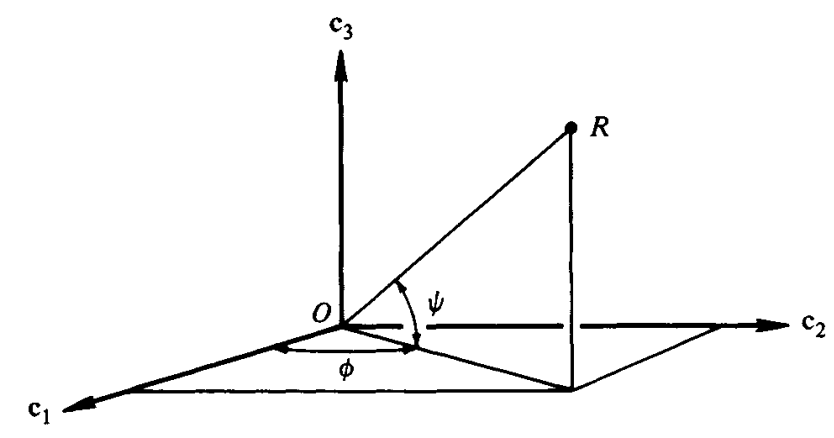
\includegraphics[width=0.8\textwidth]{Figure/例题2.3.png}
        \caption{例题2.3}
        \label{fig:间接定向法例题}
    \end{figure}

    两个航天器 $A$、$B$ 同时对两颗恒星 $P$、$Q$ 进行观测，以生成用于确定 $A$ 与 $B$ 之间相对姿态所需的数据。观测内容为测量图~\eqref{fig:间接定向法例题}中所示的角度 $\phi$ 和 $\psi$，其中 $O$ 表示 $A$ 中或 $B$ 中固定的点，$R$ 是 $P$ 或 $Q$，$\mathbf{c}_1,\mathbf{c}_2,\mathbf{c}_3$ 是 $A$ 中或 $B$ 中固定的右手正交单位向量。表~\ref{tab:1.5.1} 给出了这些角度的数值，要求确定方向余弦矩阵 $\bm{A}$。
\end{example}

\begin{solution}
若定义 $\mathbf{R}$ 为由 $O$ 指向 $R$ 的单位向量（参见图~\eqref{fig:间接定向法例题}），则
$$
\mathbf{R}=\cos\psi\cos\phi\,\mathbf{c}_1+\cos\psi\sin\phi\,\mathbf{c}_2+\sin\psi\,\mathbf{c}_3
$$
因此令 $\mathbf{p}$、$\mathbf{q}$ 分别为由 $O$ 指向 $P$ 和指向 $Q$ 的单位向量，结合表~\ref{tab:1.5.1}，可分别用 $\mathbf{a}_1,\mathbf{a}_2,\mathbf{a}_3$ 和 $\mathbf{b}_1,\mathbf{b}_2,\mathbf{b}_3$ 表达这两个向量（结果列于表~\ref{tab:1.5.2} 的第 1、2 行）；由此可计算 $\mathbf{r}$（见式~\eqref{eq:定义式}）、$\mathbf{q}\times\mathbf{r}$ 和 $\mathbf{r}\times\mathbf{p}$。

\begin{table}[H]
\centering
\caption{$\phi$ 和 $\psi$ 的角度（单位：度）}
\label{tab:1.5.1}
\begin{tabular}{|c|cc|cc|}
\hline
 & \multicolumn{2}{c|}{$P$} & \multicolumn{2}{c|}{$Q$} \\
\cline{2-5}
 & $\phi$ & $\psi$ & $\phi$ & $\psi$ \\
\hline
$\mathbf{c}_i = \mathbf{a}_i$ & 90 & 45 & 30  & 0  \\
$\mathbf{c}_i = \mathbf{b}_i$ & 135 & 0  & 90  & 60 \\
\hline
\end{tabular}
\end{table}

\begin{table}[H]
\centering
\caption{出现在间接定向法中的向量}
\label{tab:1.5.2}
\begin{tabular}{|c|c|c|c|c|c|c|c|c|}
\hline
\multirow{2}{*}{行} & \multirow{2}{*}{向量} & \multicolumn{3}{c|}{在 $A$ 中} & & \multicolumn{3}{c|}{在 $B$ 中} \\
\cline{3-5}\cline{7-9}
 & & $\mathbf{a}_1$ & $\mathbf{a}_2$ & $\mathbf{a}_3$ & & $\mathbf{b}_1$ & $\mathbf{b}_2$ & $\mathbf{b}_3$ \\
\hline
1 & $\mathbf{p}$ & $0$ & $\frac{\sqrt{2}}{2}$ & $\frac{\sqrt{2}}{2}$ & & $-\frac{\sqrt{2}}{2}$ & $\frac{\sqrt{2}}{2}$ & $0$ \\
2 & $\mathbf{q}$ & $\frac{\sqrt{3}}{2}$ & $\frac{1}{2}$ & $0$ & & $0$ & $\frac{1}{2}$ & $\frac{\sqrt{3}}{2}$ \\
3 & $\mathbf{r}=\mathbf{p}\times\mathbf{q}$ & $-\frac{\sqrt{6}}{4}$ & $\frac{\sqrt{6}}{4}$ & $-\frac{\sqrt{6}}{4}$ & & $\frac{\sqrt{2}}{4}$ & $\frac{\sqrt{2}}{4}$ & $-\frac{\sqrt{2}}{4}$ \\
4 & $\mathbf{q}\times\mathbf{r}$ & $\frac{\sqrt{3}}{2}$ & $\frac{1}{4}$ & $-\frac{1}{4}$ & & $0$ & $\frac{1}{2}$ & $\frac{\sqrt{3}}{2}$ \\
5 & $\mathbf{r}\times\mathbf{p}$ & $-\frac{\sqrt{6}}{8}$ & $\frac{3\sqrt{2}}{8}$ & $\frac{\sqrt{2}}{2}$ & & $-\frac{\sqrt{2}}{2}$ & $\frac{\sqrt{2}}{2}$ & $0$ \\
\hline
\end{tabular}
\end{table}

由表~\ref{tab:1.5.2} 第 3 行可得
$$
\mathbf{r}^{2}=\frac{2}{16}+\frac{6}{16}+\frac{6}{16}=\frac{7}{8}
$$
将各项代入式~\eqref{eq:定义式}，即得
$$
\begin{aligned}
\bm{\sigma}
=&\;\frac{1}{7/8}\Big[
\bigl(-\tfrac{\sqrt{2}}{4}\mathbf{a}_1+\tfrac{\sqrt{6}}{4}\mathbf{a}_2-\tfrac{\sqrt{6}}{4}\mathbf{a}_3\bigr)\bigl(\tfrac{\sqrt{6}}{4}\mathbf{b}_1+\tfrac{\sqrt{6}}{4}\mathbf{b}_2-\tfrac{\sqrt{2}}{4}\mathbf{b}_3\bigr)\\
&+\bigl(-\tfrac{\sqrt{6}}{8}\mathbf{a}_1+\tfrac{3\sqrt{2}}{8}\mathbf{a}_2+\tfrac{\sqrt{2}}{2}\mathbf{a}_3\bigr)\bigl(-\tfrac{\sqrt{2}}{2}\mathbf{b}_1+\tfrac{\sqrt{2}}{2}\mathbf{b}_2+0\mathbf{b}_3\bigr)\\
&+\bigl(\tfrac{\sqrt{3}}{2}\mathbf{a}_1+\tfrac{1}{4}\mathbf{a}_2-\tfrac{1}{4}\mathbf{a}_3\bigr)\bigl(0\mathbf{b}_1+\tfrac{1}{2}\mathbf{b}_2+\tfrac{\sqrt{3}}{2}\mathbf{b}_3\bigr)\Big]
\end{aligned}
$$
由式~\eqref{eq:间接定向法:aij} 可逐元计算：
$$
\begin{aligned}
a_{11}=\mathbf{a}_1\cdot\bm{\sigma}\cdot\mathbf{b}_1
&=\bigl(-\tfrac{\sqrt{2}}{4}\cdot\tfrac{\sqrt{6}}{4}+\tfrac{\sqrt{6}}{8}\cdot\tfrac{\sqrt{2}}{2}\bigr)\Big/\tfrac{7}{8}=0
\\[4pt]
a_{12}=\mathbf{a}_1\cdot\bm{\sigma}\cdot\mathbf{b}_2
&=\bigl(-\tfrac{\sqrt{2}}{4}\cdot\tfrac{\sqrt{6}}{4}-\tfrac{\sqrt{6}}{8}\cdot\tfrac{\sqrt{2}}{2}+\tfrac{\sqrt{3}}{2}\cdot\tfrac{1}{2}\bigr)\Big/\tfrac{7}{8}=0
\\[4pt]
a_{13}=\mathbf{a}_1\cdot\bm{\sigma}\cdot\mathbf{b}_3
&=\bigl(\tfrac{\sqrt{2}}{4}\cdot\tfrac{\sqrt{2}}{4}+\tfrac{\sqrt{3}}{2}\cdot\tfrac{\sqrt{3}}{2}\bigr)\Big/\tfrac{7}{8}=1
\end{aligned}
$$
类似地计算其余元，最终得方向余弦矩阵
$$
\bm{A}=\begin{bmatrix}0 & 0 & 1\\ 0 & 1 & 0\\ -1 & 0 & 0\end{bmatrix}
$$
这表明 $A$ 系是 $B$ 系绕 $\mathbf{b}_2$ 轴旋转 $90^\circ$（右手定则）所得到的。
\end{solution}

%=============================================================
\section{小角度旋转}
其实就是近似问题。当一个简单旋转足够小，以至于转角$\theta$的二次幂和高次幂均可忽略时，可以将$\sin\theta$和$\tan \theta$近似处理为$\theta$。将$\cos\theta$处理为1。

于是式~\eqref{eq:simple_rotation_formula}可以转化为：
\begin{equation}
    \mathbf{b}=\mathbf{a}-\mathbf{a}\times\bm{\lambda}\theta
\end{equation}
利用叉乘矩阵，$\mathbf{a}\times\bm{\lambda}=-\tilde{\bm{\lambda}}\,\mathbf{a}$，故上式可写成
\begin{equation}
    \mathbf{b}=(\bm{I}+\tilde{\bm{\lambda}}\theta)\,\mathbf{a}.
\end{equation}
还有式~\eqref{eq:旋转矩阵的代数运算表示}可以转化为：
\begin{equation}
    \bm{A} \triangleq \bm{U} - (\bm{U}\times\bm{\lambda})\theta
\end{equation}
同样的，欧拉参数和罗德里格斯参数也可以进行相应的转化：
\begin{equation}
        \begin{aligned}
            &\bm{\epsilon}=\frac{1}{2} \bm{\lambda}\theta \\
            &\epsilon_4 = 1
        \end{aligned}
\end{equation}

\begin{equation}
    \bm{\rho} = \frac{1}{2}\bm{\lambda}\theta
\end{equation}
关于叉乘矩阵 $\tilde{\bm{q}}$ 的定义见数学基础（式~\eqref{eq:矩阵:叉乘矩阵}）。

%=============================================================
\section{螺旋运动}
之前的内容都是关于怎么描述物体的旋转的。我们知道，在刚刚接触力学时，我们先学习点的运动，就是位移（displacement）。

\begin{mydefinition}{位移}
    如果点 $P_1$ 和 $P_2$ 在参考系 $A$ 中固定，而点 $P$ 从 $P_1$ 移动到 $P_2$，则称 $P$ 在 $A$ 中发生了位移，且 $P_2$ 相对于 $P_1$ 的位矢称为 $P$ 在 $A$ 中的位移矢量。

    当刚体 $B$ 的各点在参考系 $A$ 中发生位移时，我们称之为 $B$ 在 $A$ 中的位移；若 $B$ 在 $A$ 中的所有点的位移矢量都相等，则称此位移为 $B$ 在 $A$ 中的平移（translation）。
\end{mydefinition}
刚体 $B$ 在参考系 $A$ 中的任意位移，都可以通过依次对 $B$ 进行平移来实现：选择 $B$ 上任意一点 $P$，将其从初始位置移动至终止位置，再进行一次简单旋转，在此过程中 $P$ 在 $A$ 中保持不动。简单旋转的旋转矩阵、欧拉参数和罗德里格斯向量都与基点的选择无关，但基点的位移矢量则取决于该选择。当基点的位移矢量与旋转变换的罗德里格斯矢量平行时，也就是和转轴矢量平行时，该位移便可通过螺旋运动实现。
\begin{figure}[H]
    \centering
    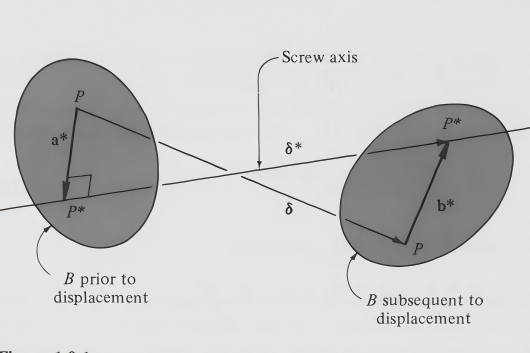
\includegraphics[width=0.8\textwidth]{Figure/螺旋运动.png}
        \caption{螺旋运动}
        \label{fig:螺旋运动}
\end{figure}

\begin{myTheorem}{螺旋运动定理}
刚体 $B$ 在参考系 $A$ 中的任意位移，都可以通过螺旋运动来实现。换句话说，总能找到一个基点，其位移矢量与 $B$ 在 $A$ 中位移所对应的简单旋转的罗德里格斯矢量平行。事实上，存在无限多个这样的基点，它们都位于一条与罗德里格斯矢量平行的直线上，这条直线称为螺杆轴；而所有位于螺杆轴上的 $B$ 点的位移矢量都相等，因此可以用一个向量（即螺杆平移矢量）来表示。此外，螺杆平移矢量的模长不小于任何不在螺杆轴上的基点的位移矢量的模长。若 $\bm{\delta}$ 是任意基点 $P$ 的位移矢量，$\bm{\rho}$ 是在 $A$ 中对 $B$ 进行位移所对应的旋转变换的罗德里格斯矢量，且 $P^*$ 是位于螺杆轴上的 $B$ 点（见图~\ref{fig:螺旋运动}），则在 $B$ 在 $A$ 中发生位移前，$P^*$ 相对于 $P$ 的位置矢量 $\bm{a}^*$ 满足以下方程：
\begin{equation}
    \label{eq:螺旋运动:a_star公式}
    \bm{a}^* = \frac{\bm{\rho} \times \bm{\delta} + (\bm{\rho} \times \bm{\delta}) \times \bm{\rho}}{2\bm{\rho}^2} + \mu \bm{\rho}
\end{equation}
其中 $\mu$ 取决于 $P^*$ 的选择；而螺杆平移矢量 $\bm{\delta}^*$ 由以下公式给出：
$$
\bm{\delta}^* = \frac{\bm{\rho} \cdot \bm{\delta}}{\bm{\rho}^2} \bm{\rho}
$$
\end{myTheorem}
\begin{proof}
    若 $P^*$ 和 $P$ 均为任意选取的点，且 $\bm{a}^*$ 是在 $B$ 在 $A$ 中发生位移前，$P^*$ 相对于 $P$ 的位置矢量，$\bm{b}^*$ 是在此位移之后 $P^*$ 相对于 $P$ 的位置矢量，则 $P^*$ 的位移矢量 $\bm{\delta}^*$ 可表示为（见图~\ref{fig:螺旋运动}）
\begin{equation}
    \bm{\delta}^* = \bm{\delta} + \bm{b}^* - \bm{a}^*
    \label{eq:螺旋运动:delta_star定义}
\end{equation}
其中 $\bm{\delta}$ 是点 $P$ 的位移矢量；且由式~\eqref{eq:罗德里格斯向量表示的和差关系}
\begin{equation}
    \bm{b}^* - \bm{a}^* = \bm{\rho} \times (\bm{a}^* + \bm{b}^*)
    \label{eq:螺旋运动:差值关系}
\end{equation}
代入得
\begin{equation}
    \bm{\delta}^* = \bm{\delta} + \bm{\rho} \times (\bm{a}^* + \bm{b}^*)
    \label{eq:螺旋运动:delta_star代入}
\end{equation}
因此，若要选择 $P^*$ 使得 $\bm{\delta}^*$ 与 $\bm{\rho}$ 平行（此时 $\bm{\rho} \times \bm{\delta}^*$ 等于零），则 $\bm{a}^*$ 必须满足方程：
\begin{equation}
    \bm{\rho} \times \bm{\delta} + \bm{\rho} \times [\bm{\rho} \times (\bm{a}^* + \bm{b}^*)] = 0
    \label{eq:螺旋运动:平行条件}
\end{equation}
或等价地，
\begin{equation}
    \bm{\rho} \times \bm{\delta} + \bm{\rho} \cdot (\bm{a}^* + \bm{b}^*) \bm{\rho} - \bm{\rho}^2 (\bm{a}^* + \bm{b}^*) = 0
    \label{eq:螺旋运动:三重积展开}
\end{equation}
故
\begin{equation}
    \bm{a}^* + \bm{b}^* = \frac{\bm{\rho} \times \bm{\delta}}{\bm{\rho}^2} + \frac{\bm{\rho} \cdot (\bm{a}^* + \bm{b}^*)}{\bm{\rho}^2} \bm{\rho}
    \label{eq:螺旋运动:和矢表达式}
\end{equation}
然后又有：
\begin{equation}
    \bm{\delta}^* = \bm{\delta} + \bm{\rho} \times \frac{\bm{\rho} \times \bm{\delta}}{\bm{\rho}^2} = \frac{\bm{\rho} \cdot \bm{\delta}}{\bm{\rho}^2} \bm{\rho}
    \label{eq:螺旋运动:delta_star公式}
\end{equation}
和
\begin{equation}
    \bm{b}^* - \bm{a}^* = \bm{\rho} \times \frac{\bm{\rho} \times \bm{\delta}}{\bm{\rho}^2}
    \label{eq:螺旋运动:差值结果}
\end{equation}
联立式~\eqref{eq:螺旋运动:和矢表达式}和式~\eqref{eq:螺旋运动:差值结果}，可得
\begin{equation}
    \bm{a}^* = \frac{\bm{\rho} \times \bm{\delta} + (\bm{\rho} \times \bm{\delta}) \times \bm{\rho}}{2\bm{\rho}^2} + \frac{\bm{\rho} \cdot \bm{a}^*}{\bm{\rho}^2 }\bm{\rho}
\end{equation}可得式~\eqref{eq:螺旋运动:a_star公式}

然后由式~\eqref{eq:螺旋运动:delta_star公式}，两边取模，可得
\begin{equation}
    \left|\bm{\delta}^*\right| = \left|\frac{\bm{\rho} \cdot \bm{\delta}}{\bm{\rho}^2} \bm{\rho}\right|=\frac{\left|\bm{\rho} \cdot \bm{\delta}\right|}{\left|\bm{\rho}\right|}\leqslant \left|\bm{\delta}\right|
\end{equation}
于是螺杆平移矢量的模长不小于任何不在螺杆轴上的基点的位移矢量的模长。
\end{proof}

%=============================================================
\section{角速度矩阵}
若 $\mathbf{a}_1,\mathbf{a}_2,\mathbf{a}_3$ 与 $\mathbf{b}_1,\mathbf{b}_2,\mathbf{b}_3$ 分别为固定在两个相互运动的参考系或刚体 $A$ 与 $B$ 中的两组成右手正交单位向量，则由式~\eqref{eq:方向余弦的定义} 定义的方向余弦矩阵 $\bm{A}$ 及其元素 $\bar{a}_{ij}\;(i,j=1,2,3)$ 均为时间 $t$ 的函数。$\bm{A}$ 的时间导数记为 $\dot{\bm{A}}$，由各元素 $a_{ij}\;(i,j=1,2,3)$ 的时间导数 $\dot{a}_{ij}$ 按如下方式定义：
\begin{equation}
    \dot{\bm{A}}\triangleq\begin{bmatrix}
        \dot{a}_{11}&\dot{a}_{12}&\dot{a}_{13}\\
        \dot{a}_{21}&\dot{a}_{22}&\dot{a}_{23}\\
        \dot{a}_{31}&\dot{a}_{32}&\dot{a}_{33}
    \end{bmatrix}
    \label{eq:角速度矩阵:微分定义}
\end{equation}
\begin{myTheorem}{角速度矩阵的性质}
$\dot{\bm{A}}$ 可以表示为 $\bm{A}$ 与某个反对称矩阵的乘积，该反对称矩阵称为 $B$ 在 $A$ 中的角速度矩阵，定义为
\begin{equation}
    \bm{\tilde{\omega}}\triangleq\bm{A}^{\mathrm{T}}\dot{\bm{A}}
    \label{eq:角速度矩阵:定义}
\end{equation}
换言之，若 $\bm{\tilde{\omega}}$ 按式~\eqref{eq:角速度矩阵:定义} 定义，则
\begin{equation}
    \dot{\bm{A}}=\bm{A}\,\bm{\tilde{\omega}}
    \label{eq:角速度矩阵:基本关系}
\end{equation}
\end{myTheorem}

若按照叉乘矩阵的记号约定（见式~\eqref{eq:矩阵:叉乘矩阵}）引入三个时间函数 $\omega_1(t),\omega_2(t),\omega_3(t)$，把 $\bm{\tilde{\omega}}$ 表示为
\begin{equation}
    \bm{\tilde{\omega}}=\begin{bmatrix}
        0&-\omega_3&\omega_2\\
        \omega_3&0&-\omega_1\\
        -\omega_2&\omega_1&0
    \end{bmatrix}
    \label{eq:角速度矩阵:反对称形式}
\end{equation}
则 $\omega_1,\omega_2,\omega_3$ 由下式给出：
\begin{equation}
    \begin{aligned}
        \omega_{1}&=a_{13}\dot{a}_{12}+a_{23}\dot{a}_{22}+a_{33}\dot{a}_{32}\\
        \omega_{2}&=a_{21}\dot{a}_{23}+a_{31}\dot{a}_{33}+a_{11}\dot{a}_{13}\\
        \omega_{3}&=a_{32}\dot{a}_{31}+a_{12}\dot{a}_{11}+a_{22}\dot{a}_{21}
    \end{aligned}
    \label{eq:角速度矩阵:分量公式}
\end{equation}

在引入 $\eta_{ijk}$ 之后，这些方程可以写得更简洁。定义
\begin{equation}
    \eta_{ijk}\triangleq\frac{1}{2}\epsilon_{ijk}(\epsilon_{ijk}+1)\quad(i,j,k=1,2,3)
    \label{eq:角速度矩阵:eta定义}
\end{equation}
其中 $\epsilon_{ijk}$ 由式~\eqref{eq:epsilon_ijk定义} 给出。（当下标呈循环次序时 $\eta_{ijk}$ 等于 1，否则等于 0。）对重复下标采用求和约定，式~\eqref{eq:角速度矩阵:分量公式} 便可改写为
\begin{equation}
    \omega_{i}=\eta_{igh}\dot{a}_{jg}a_{jh}\quad(i=1,2,3)
    \label{eq:角速度矩阵:紧凑形式}
\end{equation}
类似地，式~\eqref{eq:角速度矩阵:基本关系} 可以表示为
\begin{equation}
    \dot{a}_{ij}=a_{ig}\,\omega_{h}\,\epsilon_{ghj}\quad(i,j=1,2,3)
    \label{eq:角速度矩阵:紧凑形式2}
\end{equation}
或显式地写成
\begin{equation}
    \begin{aligned}
        \dot{a}_{11}&=a_{12}\omega_{3}-a_{13}\omega_{2},\quad
        \dot{a}_{12}=a_{13}\omega_{1}-a_{11}\omega_{3},\quad
        \dot{a}_{13}=a_{11}\omega_{2}-a_{12}\omega_{1}\\
        \dot{a}_{21}&=a_{22}\omega_{3}-a_{23}\omega_{2},\quad
        \dot{a}_{22}=a_{23}\omega_{1}-a_{21}\omega_{3},\quad
        \dot{a}_{23}=a_{21}\omega_{2}-a_{22}\omega_{1}\\
        \dot{a}_{31}&=a_{32}\omega_{3}-a_{33}\omega_{2},\quad
        \dot{a}_{32}=a_{33}\omega_{1}-a_{31}\omega_{3},\quad
        \dot{a}_{33}=a_{31}\omega_{2}-a_{32}\omega_{1}
    \end{aligned}
    \label{eq:角速度矩阵:Poisson方程}
\end{equation}
式~\eqref{eq:角速度矩阵:Poisson方程} 称为泊松运动学方程（Poisson's kinematical equations）。

\begin{proof}
    将式~\eqref{eq:角速度矩阵:定义} 两端左乘 $\bm{A}$，得
\begin{equation}
    \bm{A}\,\bm{\tilde{\omega}}=\bm{A}\,\bm{A}^{\mathrm{T}}\dot{\bm{A}}=\dot{\bm{A}}
    \label{eq:角速度矩阵:推导基本关系}
\end{equation}
与式~\eqref{eq:角速度矩阵:基本关系} 一致。

为说明按式~\eqref{eq:角速度矩阵:定义} 定义的 $\bm{\tilde{\omega}}$ 是反对称矩阵，注意到
\begin{equation}
    \bm{\tilde{\omega}}^{\mathrm{T}}+\bm{\tilde{\omega}}
    =(\bm{A}^{\mathrm{T}}\dot{\bm{A}})^{\mathrm{T}}+\bm{A}^{\mathrm{T}}\dot{\bm{A}}
    =\dot{\bm{A}}^{\mathrm{T}}\bm{A}+\bm{A}^{\mathrm{T}}\dot{\bm{A}}
    =\frac{\mathrm{d}}{\mathrm{d}t}\bigl(\bm{A}^{\mathrm{T}}\bm{A}\bigr)
    \label{eq:角速度矩阵:反对称推导}
\end{equation}
由方向余弦矩阵的正交性（性质五），$\bm{A}^{\mathrm{T}}\bm{A}=\bm{I}$，故
\begin{equation}
    \frac{\mathrm{d}}{\mathrm{d}t}\bigl(\bm{A}^{\mathrm{T}}\bm{A}\bigr)=\frac{\mathrm{d}\bm{I}}{\mathrm{d}t}=0
\end{equation}
于是
\begin{equation}
    \bm{\tilde{\omega}}^{\mathrm{T}}=-\bm{\tilde{\omega}}
    \label{eq:角速度矩阵:反对称性}
\end{equation}
即 $\bm{\tilde{\omega}}$ 为反对称矩阵。

式~\eqref{eq:角速度矩阵:分量公式} 可由式~\eqref{eq:角速度矩阵:定义} 和式~\eqref{eq:角速度矩阵:反对称形式} 直接得出，即由
\begin{equation}
    \begin{bmatrix}
        0&-\omega_{3}&\omega_{2}\\
        \omega_{3}&0&-\omega_{1}\\
        -\omega_{2}&\omega_{1}&0
    \end{bmatrix}
    =
    \begin{bmatrix}
        a_{11}&a_{21}&a_{31}\\
        a_{12}&a_{22}&a_{32}\\
        a_{13}&a_{23}&a_{33}
    \end{bmatrix}
    \begin{bmatrix}
        \dot{a}_{11}&\dot{a}_{12}&\dot{a}_{13}\\
        \dot{a}_{21}&\dot{a}_{22}&\dot{a}_{23}\\
        \dot{a}_{31}&\dot{a}_{32}&\dot{a}_{33}
    \end{bmatrix}
    \label{eq:角速度矩阵:推导分量公式}
\end{equation}
得出。

\end{proof}

%=============================================================
\section{角速度矢量}\label{sec:angular-velocity-vector}
定义向量 $\bm{\omega}$ 为
\begin{equation}
    \bm{\omega} \triangleq \omega_1\,\mathbf{b}_1 + \omega_2\,\mathbf{b}_2 + \omega_3\,\mathbf{b}_3
    \label{eq:角速度矢量:定义}
\end{equation}
其中 $\omega_i$ 与 $\mathbf{b}_i$ $(i=1,2,3)$ 的含义与角速度矩阵一节相同，则 $\bm{\omega}$ 称为 $B$ 在 $A$ 中（或相对于 $A$）的角速度。有时用更完备的符号 $\bm{\omega}_{B|A}$ 代替 $\bm{\omega}$ 更为方便。此时 $\bm{\omega}_{A|B}$ 表示 $A$ 在 $B$ 中的角速度，且有
\begin{equation}
    \bm{\omega}_{B|A} = -\bm{\omega}_{A|B}
    \label{eq:角速度矢量:反对称性}
\end{equation}

若 $\mathbf{b}_i$ 在参考系 $A$ 中的一阶时间导数记为 $\dot{\mathbf{b}}_i$，即
\begin{equation}
    \dot{\mathbf{b}}_i \triangleq \mathbf{a}_j \frac{\mathrm{d}}{\mathrm{d}t}(\mathbf{a}_j\cdot\mathbf{b}_i)\quad(i=1,2,3)
    \label{eq:角速度矢量:单位矢导数}
\end{equation}
其中对重复下标采用求和约定（即‌爱因斯坦求和约定‌），且 $\mathbf{a}_1,\mathbf{a}_2,\mathbf{a}_3$ 为固定在 $A$ 中的一组成右手正交单位向量，则 $\bm{\omega}$ 可以表示为
\begin{equation}
    \bm{\omega} = \mathbf{b}_1\,\dot{\mathbf{b}}_2\cdot\mathbf{b}_3 + \mathbf{b}_2\,\dot{\mathbf{b}}_3\cdot\mathbf{b}_1 + \mathbf{b}_3\,\dot{\mathbf{b}}_1\cdot\mathbf{b}_2
    \label{eq:角速度矢量:基本关系}
\end{equation}

当 $B$ 在 $A$ 中的运动为简单转动（见简单转动一节）时，$B$ 在 $A$ 中的角速度变为
\begin{equation}
    \bm{\omega} = \dot{\theta}\,\bm{\lambda}
    \label{eq:角速度矢量:简单转动}
\end{equation}
其中 $\theta$ 和 $\bm{\lambda}$ 的含义与简单转动一节相同。

\begin{myTheorem}{角速度的导数关系}
涉及角速度的最有用的关系之一是向量 $\bm{v}$ 在两个参考系 $A$ 与 $B$ 中的一阶时间导数之间的关系。若这两个导数分别记为 $\dfrac{\mathrm{d}\bm{v}}{\mathrm{d}t}\Big|_A$ 和 $\dfrac{\mathrm{d}\bm{v}}{\mathrm{d}t}\Big|_B$，即
\begin{equation}
    \frac{\mathrm{d}\bm{v}}{\mathrm{d}t}\Big|_A \triangleq \mathbf{a}_i\frac{\mathrm{d}}{\mathrm{d}t}(\bm{v}\cdot\mathbf{a}_i)
    \label{eq:角速度矢量:A系导数}
\end{equation}
和
\begin{equation}
    \frac{\mathrm{d}\bm{v}}{\mathrm{d}t}\Big|_B \triangleq \mathbf{b}_i\frac{\mathrm{d}}{\mathrm{d}t}(\bm{v}\cdot\mathbf{b}_i)
    \label{eq:角速度矢量:B系导数}
\end{equation}
则该关系具有如下形式：
\begin{equation}
    \frac{\mathrm{d}\bm{v}}{\mathrm{d}t}\Big|_A = \frac{\mathrm{d}\bm{v}}{\mathrm{d}t}\Big|_B + \bm{\omega}_{B|A}\times\bm{v}
    \label{eq:角速度矢量:导数关系}
\end{equation}
将此式应用于固定在 $B$ 中的向量 $\bm{\beta}$，得
\begin{equation}
    \frac{\mathrm{d}\bm{\beta}}{\mathrm{d}t}\Big|_A = \bm{\omega}_{B|A}\times\bm{\beta}
\end{equation}
由此结果可以看出，可以把 $B$ 在 $A$ 中的角速度视为一个“算子”：它作用于 $B$ 中任意固定向量时，便产生该向量在 $A$ 中的时间导数。
\end{myTheorem}
\begin{proof}
    对于 $i=2$，式~\eqref{eq:角速度矢量:单位矢导数} 中出现的标量积可以表示为方向余弦矩阵中的一个元素：
\begin{equation}
    \mathbf{a}_j\cdot\mathbf{b}_2 = a_{j2}
\end{equation}
于是
\begin{equation}
    \dot{\mathbf{b}}_2 = \mathbf{a}_1\dot{a}_{12} + \mathbf{a}_2\dot{a}_{22} + \mathbf{a}_3\dot{a}_{32}
\end{equation}
再把 $\mathbf{b}_3$ 表示为
\begin{equation}
    \mathbf{b}_3 = \mathbf{a}_1a_{13} + \mathbf{a}_2a_{23} + \mathbf{a}_3a_{33}
\end{equation}
由式~\eqref{eq:角速度矩阵:分量公式}可求得
\begin{equation}
    \dot{\mathbf{b}}_2\cdot\mathbf{b}_3 = a_{13}\dot{a}_{12} + a_{23}\dot{a}_{22} + a_{33}\dot{a}_{32} = \omega_1
\end{equation}
类似地，
\begin{equation}
    \dot{\mathbf{b}}_3\cdot\mathbf{b}_1 = \omega_2,\qquad
    \dot{\mathbf{b}}_1\cdot\mathbf{b}_2 = \omega_3
\end{equation}
代入式~\eqref{eq:角速度矢量:定义}，即得式~\eqref{eq:角速度矢量:基本关系}。

当 $B$ 在 $A$ 中的运动为简单转动时，可把 $B$ 在 $A$ 中的角速度表示为
\begin{equation}
    \bm{\omega} = (\lambda_1\mathbf{b}_1 + \lambda_2\mathbf{b}_2 + \lambda_3\mathbf{b}_3)\dot{\theta}
    = (\bm{\lambda}\cdot\mathbf{b}_1\,\mathbf{b}_1 + \bm{\lambda}\cdot\mathbf{b}_2\,\mathbf{b}_2 + \bm{\lambda}\cdot\mathbf{b}_3\,\mathbf{b}_3)\dot{\theta}
    = \bm{\lambda}\dot{\theta}
\end{equation}
与式~\eqref{eq:角速度矢量:简单转动} 一致。

为建立式~\eqref{eq:角速度矢量:导数关系}，设 $\nu_{i|A}$、$\nu_{i|B}$、$\bm{\nu}_{|A}$ 和 $\bm{\nu}_{|B}$ 的含义与方向余弦一节相同（$\bm{\nu}_{|A}$、$\bm{\nu}_{|B}$ 分别为 $\bm{v}$ 在 $A$、$B$ 中的分量行阵）。则由式~\eqref{eq:角速度矢量:A系导数} 和式~\eqref{eq:方向余弦的定义}，
\begin{equation}
    \frac{\mathrm{d}\bm{v}}{\mathrm{d}t}\Big|_A
    = \dot{\nu}_{1|A}\mathbf{a}_1 + \dot{\nu}_{2|A}\mathbf{a}_2 + \dot{\nu}_{3|A}\mathbf{a}_3
    = \dot{\bm{\nu}}_{|A}\begin{bmatrix}\mathbf{a}_1 \\ \mathbf{a}_2 \\ \mathbf{a}_3\end{bmatrix}
\end{equation}
现在，
\begin{equation}
    \dot{\bm{\nu}}_{|A} = \frac{\mathrm{d}}{\mathrm{d}t}\bigl(\bm{\nu}_{|B}\bm{A}^{\mathrm{T}}\bigr)
    = \dot{\bm{\nu}}_{|B}\bm{A}^{\mathrm{T}} + \bm{\nu}_{|B}\dot{\bm{A}}^{\mathrm{T}}
\end{equation}
且由式~\eqref{eq:direction_cosine_matrix}，
\begin{equation}
    \begin{bmatrix}\mathbf{a}_1 \\ \mathbf{a}_2 \\ \mathbf{a}_3\end{bmatrix}
    = \bm{A}\begin{bmatrix}\mathbf{b}_1 \\ \mathbf{b}_2 \\ \mathbf{b}_3\end{bmatrix}
\end{equation}
于是，
\begin{equation}
    \frac{\mathrm{d}\bm{v}}{\mathrm{d}t}\Big|_A
    = \dot{\bm{\nu}}_{|B}\bm{A}^{\mathrm{T}}\bm{A}\begin{bmatrix}\mathbf{b}_1 \\ \mathbf{b}_2 \\ \mathbf{b}_3\end{bmatrix}
    + \bm{\nu}_{|B}\dot{\bm{A}}^{\mathrm{T}}\bm{A}\begin{bmatrix}\mathbf{b}_1 \\ \mathbf{b}_2 \\ \mathbf{b}_3\end{bmatrix}
\end{equation}
由方向余弦矩阵的正交性（性质五），$\bm{A}^{\mathrm{T}}\bm{A}=\bm{I}$；又由式~\eqref{eq:角速度矩阵:定义}，$\dot{\bm{A}}^{\mathrm{T}}\bm{A}=(\bm{A}^{\mathrm{T}}\dot{\bm{A}})^{\mathrm{T}}=\bm{\tilde{\omega}}^{\mathrm{T}}$，故
\begin{equation}
    \frac{\mathrm{d}\bm{v}}{\mathrm{d}t}\Big|_A
    = \dot{\bm{\nu}}_{|B}\begin{bmatrix}\mathbf{b}_1 \\ \mathbf{b}_2 \\ \mathbf{b}_3\end{bmatrix}
    + \bm{\nu}_{|B}\bm{\tilde{\omega}}^{\mathrm{T}}\begin{bmatrix}\mathbf{b}_1 \\ \mathbf{b}_2 \\ \mathbf{b}_3\end{bmatrix}
\end{equation}
此外，由式~\eqref{eq:角速度矢量:B系导数}，
\begin{equation}
    \dot{\bm{\nu}}_{|B}\begin{bmatrix}\mathbf{b}_1 \\ \mathbf{b}_2 \\ \mathbf{b}_3\end{bmatrix} = \frac{\mathrm{d}\bm{v}}{\mathrm{d}t}\Big|_B
\end{equation}
而由式~\eqref{eq:角速度矢量:定义} 和式~\eqref{eq:角速度矩阵:反对称形式} 可得
\begin{equation}
    \bm{\nu}_{|B}\bm{\tilde{\omega}}^{\mathrm{T}}\begin{bmatrix}\mathbf{b}_1 \\ \mathbf{b}_2 \\ \mathbf{b}_3\end{bmatrix} = \bm{\omega}_{B|A}\times\bm{v}
\end{equation}
因此，
\begin{equation}
    \frac{\mathrm{d}\bm{v}}{\mathrm{d}t}\Big|_A = \frac{\mathrm{d}\bm{v}}{\mathrm{d}t}\Big|_B + \bm{\omega}_{B|A}\times\bm{v}
\end{equation}
此即式~\eqref{eq:角速度矢量:导数关系}。

最后，式~\eqref{eq:角速度矢量:反对称性} 可由如下事实得出：在式~\eqref{eq:角速度矢量:导数关系} 中交换 $A$ 和 $B$，得
\begin{equation}
    \frac{\mathrm{d}\bm{v}}{\mathrm{d}t}\Big|_B = \frac{\mathrm{d}\bm{v}}{\mathrm{d}t}\Big|_A + \bm{\omega}_{A|B}\times\bm{v}
\end{equation}
将此式与式~\eqref{eq:角速度矢量:导数关系} 对应相加，得
\begin{equation}
    \frac{\mathrm{d}\bm{v}}{\mathrm{d}t}\Big|_A + \frac{\mathrm{d}\bm{v}}{\mathrm{d}t}\Big|_B
    = \frac{\mathrm{d}\bm{v}}{\mathrm{d}t}\Big|_B + \frac{\mathrm{d}\bm{v}}{\mathrm{d}t}\Big|_A
    + (\bm{\omega}_{B|A} + \bm{\omega}_{A|B})\times\bm{v}
\end{equation}
即
\begin{equation}
    (\bm{\omega}_{B|A} + \bm{\omega}_{A|B})\times\bm{v} = \bm{0}
\end{equation}
此式对所有 $\bm{v}$ 均成立，当且仅当
\begin{equation}
    \bm{\omega}_{B|A} = -\bm{\omega}_{A|B}
\end{equation}

\end{proof}

\blocksep
\begin{example}
    当点 $P$ 在固定在参考系 $A$ 中的空间曲线 $C$ 上运动时（见图~\ref{fig:角速度矢量例题}），可以通过令 $\bm{p}$ 为 $P$ 相对于固定在 $C$ 上的点 $P_0$ 的位矢，并把 $\mathbf{b}_1,\mathbf{b}_2,\mathbf{b}_3$ 定义为
    \begin{equation}
        \mathbf{b}_1 \triangleq \bm{p}'
    \end{equation}
    \begin{equation}
        \mathbf{b}_2 \triangleq \frac{\bm{p}''}{|\bm{p}''|}
    \end{equation}
    \begin{equation}
        \mathbf{b}_3 \triangleq \bm{p}'\times\frac{\bm{p}''}{|\bm{p}''|}
    \end{equation}
    \begin{figure}[H]
        \centering
        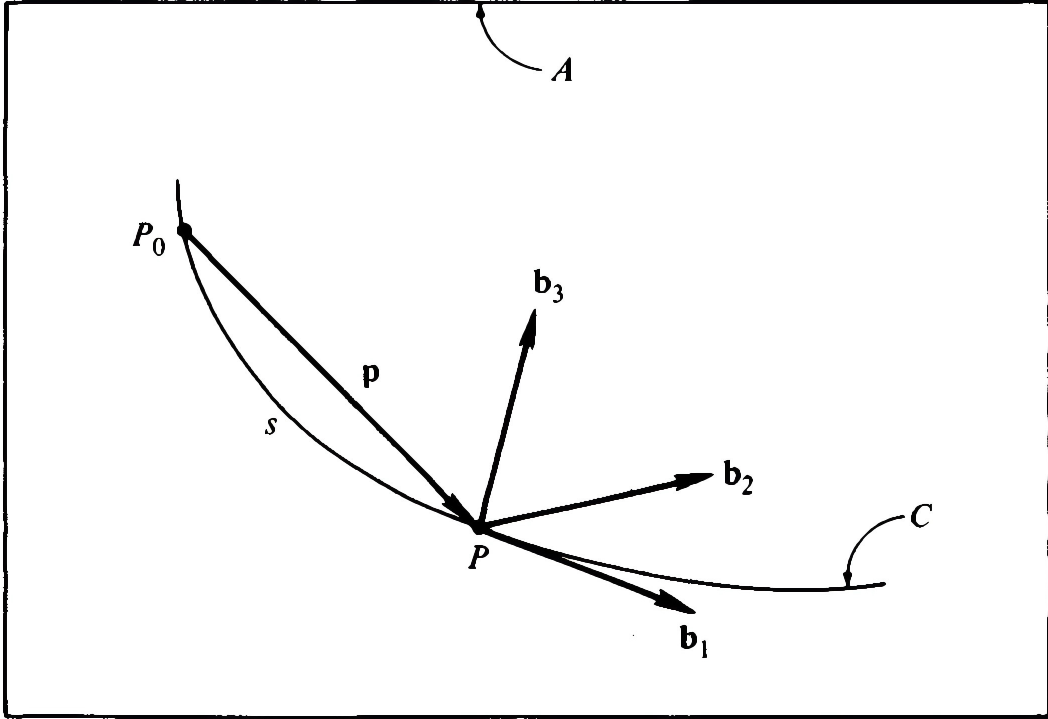
\includegraphics[width=0.8\textwidth]{Figure/角速度矢量例题.png}
            \caption{角速度矢量例题}
            \label{fig:角速度矢量例题}
    \end{figure}
    从而生成一组成右手正交单位向量。其中撇号表示在 $A$ 中对相对于 $P_0$ 的弧长位移 $s$ 求导。向量 $\mathbf{b}_1$ 称为 $C$ 在 $P$ 处的切向量（tangent vector），$\mathbf{b}_2$ 称为主法向量（principal normal vector），$\mathbf{b}_3$ 称为副法向量（binormal vector）；$\mathbf{b}_1,\mathbf{b}_2,\mathbf{b}_3$ 对 $s$ 的导数由 Serret--Frénet（塞尔-弗雷内）公式给出
    \begin{equation}
        \mathbf{b}_1' = \frac{\mathbf{b}_2}{\rho}
    \end{equation}
    \begin{equation}
        \mathbf{b}_2' = -\frac{\mathbf{b}_1}{\rho} + \lambda\mathbf{b}_3
    \end{equation}
    \begin{equation}
        \mathbf{b}_3' = -\lambda\mathbf{b}_2
    \end{equation}
    其中 $\rho$ 与 $\lambda$ 定义为
    \begin{equation}
        \rho \triangleq \frac{1}{|\bm{p}''|}
    \end{equation}
    和
    \begin{equation}
        \lambda \triangleq \rho^{2}\,\bm{p}'\cdot\bm{p}''\times\bm{p}^{\prime\prime\prime}
    \end{equation}
    分别称为 $C$ 在 $P$ 处的主曲率半径和 $C$ 在 $P$ 处的挠率（torsion）。

    若 $B$ 为使得 $\mathbf{b}_1,\mathbf{b}_2,\mathbf{b}_3$ 固定于其中的参考系，则 $B$ 在 $A$ 中的角速度 $\bm{\omega}$ 可由式~\eqref{eq:角速度矢量:基本关系} 结合 Serret--Frénet 公式还有链式法则用 $\mathbf{b}_1,\mathbf{b}_2,\mathbf{b}_3$、$\rho$、$\lambda$ 和 $\dot{s}$ 表示：
    \begin{equation}
        \dot{\mathbf{b}}_1 = \mathbf{b}_1'\dot{s} = \frac{\mathbf{b}_2\,\dot{s}}{\rho}
    \end{equation}
    \begin{equation}
        \dot{\mathbf{b}}_2 = \left(-\frac{\mathbf{b}_1}{\rho} + \lambda\mathbf{b}_3\right)\dot{s}
    \end{equation}
    \begin{equation}
        \dot{\mathbf{b}}_3 = -\lambda\mathbf{b}_2\dot{s}
    \end{equation}
    \begin{equation}
        \dot{\mathbf{b}}_1\cdot\mathbf{b}_2 = \frac{\dot{s}}{\rho},\qquad
        \dot{\mathbf{b}}_2\cdot\mathbf{b}_3 = \lambda\dot{s},\qquad
        \dot{\mathbf{b}}_3\cdot\mathbf{b}_1 = 0
    \end{equation}
    从而得到
    \begin{equation}
        \bm{\omega} = \left(\lambda\mathbf{b}_1 + \frac{\mathbf{b}_3}{\rho}\right)\dot{s}
        \label{eq:角速度矢量:SerretFrenet角速度}
    \end{equation}
    由此可以看出，“挠率”一词用于 $\lambda$ 在此语境下十分贴切。


\end{example}

%=============================================================
\section{角速度分量}\label{sec:angular-velocity-components}
\begin{myTheorem}{角速度分量的几何解释}
式~\eqref{eq:角速度矢量:定义} 中的角速度分量 $\omega_i\mathbf{b}_i$ 可赋予几何意义。一般难以通过指定两个参考系来给出 $\omega_i$ 的物理解释（如第~\ref{sec:angular-velocity-vector}~节例题中 $\lambda\dot{s}\,\mathbf{b}_1$、$(\dot{s}/\rho)\,\mathbf{b}_3$ 所示），但 $\omega_1,\omega_2,\omega_3$ 可理解为三个角的一阶时间导数的空间平均值：设 $\bm{\alpha}$ 为固定在 $A$ 中的单位向量，$\bm{\beta}_i$ 为 $\bm{\alpha}$ 在垂直于 $\mathbf{b}_i$ 的平面上的正交投影，$\theta_1$、$\theta_2$、$\theta_3$ 分别为 $\bm{\beta}_1$ 与 $\bm{\beta}_3$、$\bm{\beta}_2$ 与 $\bm{\beta}_1$、$\bm{\beta}_3$ 与 $\bm{\beta}_2$ 的夹角。令 $S$ 为以 $O$ 为球心的单位球面，$P$ 为 $S$ 上位矢平行于 $\bm{\alpha}$ 的点，则 $\dot{\theta}_i$ 是 $P$ 的函数，定义其球面平均为
\begin{equation}
    \overline{\dot{\theta}}_i \triangleq \frac{1}{4\pi}\int \dot{\theta}_i\,\mathrm{d}\sigma \quad (i=1,2,3)
    \label{eq:角速度分量:平均导数定义}
\end{equation}
其中 $\mathrm{d}\sigma$ 是 $S$ 上 $P$ 处的面积微元。于是
\begin{equation}
    \omega_i = \overline{\dot{\theta}}_i \quad (i=1,2,3)
    \label{eq:角速度分量:主要结论}
\end{equation}
\end{myTheorem}
% 角速度分量的几何解释（ω_i = 平均 θ̇_i）
% 用法：在正文中 % 角速度分量的几何解释（ω_i = 平均 θ̇_i）
% 用法：在正文中 % 角速度分量的几何解释（ω_i = 平均 θ̇_i）
% 用法：在正文中 \input{Figure/角速度分量图解}
% 依赖：preamble.tex 已加载 tikz 及库 {angles, quotes, arrows.meta}
% 说明：屏幕投影取 b1 指向右下、b2 指向左下、b3 竖直向上；
%       β_i 为 α 在垂直于 b_i 的平面（b1b2/b1b3/b2b3 面）上的正交投影。
%       所有文字标签均加白底，避免与线段、圆弧相互叠压。
\begin{figure}[htbp]
    \centering
    \begin{tikzpicture}[
        >=Stealth,
        scale=0.95,
        axis/.style={thick, ->},
        shadow/.style={dashed, line width=0.8pt},
        lbl/.style={fill=white, inner sep=1.5pt},
        every node/.style={font=\small}
    ]
        \coordinate (O)  at (0,0);
        \coordinate (B1) at (2.208,-0.912);
        \coordinate (B2) at (-2.208,-0.912);
        \coordinate (B3) at (0,2.4);
        \coordinate (P)  at (-0.199,0.650);
        \coordinate (P1) at (-1.259,1.088);
        \coordinate (P2) at (1.060,1.170);
        \coordinate (P3) at (-0.199,-0.958);

        % 三个坐标平面（⊥ b3 / ⊥ b2 / ⊥ b1）
        \fill[gray!12]  (O) -- (B1) -- (B2) -- cycle;
        \fill[blue!7]   (O) -- (B1) -- (B3) -- cycle;
        \fill[green!7]  (O) -- (B2) -- (B3) -- cycle;

        % 单位球面 S
        \fill[blue!4] (O) circle (2.4);
        \draw (O) circle (2.4);

        % 投影关系：β_i 是 α 在相应平面上的正交投影（虚点线）
        \draw[dotted, gray] (P) -- (P1);
        \draw[dotted, gray] (P) -- (P2);
        \draw[dotted, gray] (P) -- (P3);

        % 投影向量 β_1, β_2, β_3
        \draw[shadow, orange]  (O) -- (P1);
        \draw[shadow, blue!60] (O) -- (P2);
        \draw[shadow, red!60]  (O) -- (P3);
        \fill[orange]  (P1) circle (1.6pt);
        \fill[blue!60] (P2) circle (1.6pt);
        \fill[red!60]  (P3) circle (1.6pt);

        % 轴 b_1, b_2, b_3
        \draw[axis] (O) -- (B1);
        \draw[axis] (O) -- (B2);
        \draw[axis] (O) -- (B3);

        % 向量 α 及球面上的点 P
        \draw[thick, ->] (O) -- (P);
        \fill (P) circle (2pt);

        % 夹角 θ_1, θ_2, θ_3（仅画弧，标签单独放置避免叠压）
        \pic[draw, orange,  angle radius=0.75cm] {angle = P1--O--P3};
        \pic[draw, blue!60, angle radius=0.6cm]  {angle = P2--O--P1};
        \pic[draw, red!60,  angle radius=0.6cm]  {angle = P3--O--P2};

        % ---- 文字标签（白底，位置经校核无重叠）----
        \node[lbl, below right]            at (B1) {$\mathbf{b}_1$};
        \node[lbl, below left]             at (B2) {$\mathbf{b}_2$};
        \node[lbl, above]                  at (B3) {$\mathbf{b}_3$};
        \node[lbl, above left,  orange]    at (P1) {$\boldsymbol{\beta}_1$};
        \node[lbl, above right, blue!60]   at (P2) {$\boldsymbol{\beta}_2$};
        \node[lbl, below,       red!60]    at (P3) {$\boldsymbol{\beta}_3$};
        \node[lbl] at (-0.5,0.28)   {$\boldsymbol{\alpha}$};
        \node[lbl] at (0.10,0.46)   {$P$};
        \node[lbl] at (-0.30,-0.18) {$O$};
        \node[lbl, orange]  at (-1.20,-0.38) {$\theta_1$};
        \node[lbl, blue!60] at (-0.08,1.02)  {$\theta_2$};
        \node[lbl, red!60]  at (0.98,-0.62)  {$\theta_3$};

        % 结论标注
        \node[lbl, anchor=north east] at (2.1,2.0) {$\omega_i=\overline{\dot{\theta}}_i$};
    \end{tikzpicture}
    \caption{角速度分量的几何解释：$\omega_i$ 等于夹角 $\theta_i$ 的时间导数在单位球面上的空间平均值，即 $\omega_i=\overline{\dot{\theta}}_i$（$i=1,2,3$）。图中 $\boldsymbol{\beta}_i$ 为固定在 $A$ 中的单位向量 $\boldsymbol{\alpha}$ 在垂直于 $\mathbf{b}_i$ 的平面上的正交投影。}
    \label{fig:角速度分量几何解释}
\end{figure}

% 依赖：preamble.tex 已加载 tikz 及库 {angles, quotes, arrows.meta}
% 说明：屏幕投影取 b1 指向右下、b2 指向左下、b3 竖直向上；
%       β_i 为 α 在垂直于 b_i 的平面（b1b2/b1b3/b2b3 面）上的正交投影。
%       所有文字标签均加白底，避免与线段、圆弧相互叠压。
\begin{figure}[htbp]
    \centering
    \begin{tikzpicture}[
        >=Stealth,
        scale=0.95,
        axis/.style={thick, ->},
        shadow/.style={dashed, line width=0.8pt},
        lbl/.style={fill=white, inner sep=1.5pt},
        every node/.style={font=\small}
    ]
        \coordinate (O)  at (0,0);
        \coordinate (B1) at (2.208,-0.912);
        \coordinate (B2) at (-2.208,-0.912);
        \coordinate (B3) at (0,2.4);
        \coordinate (P)  at (-0.199,0.650);
        \coordinate (P1) at (-1.259,1.088);
        \coordinate (P2) at (1.060,1.170);
        \coordinate (P3) at (-0.199,-0.958);

        % 三个坐标平面（⊥ b3 / ⊥ b2 / ⊥ b1）
        \fill[gray!12]  (O) -- (B1) -- (B2) -- cycle;
        \fill[blue!7]   (O) -- (B1) -- (B3) -- cycle;
        \fill[green!7]  (O) -- (B2) -- (B3) -- cycle;

        % 单位球面 S
        \fill[blue!4] (O) circle (2.4);
        \draw (O) circle (2.4);

        % 投影关系：β_i 是 α 在相应平面上的正交投影（虚点线）
        \draw[dotted, gray] (P) -- (P1);
        \draw[dotted, gray] (P) -- (P2);
        \draw[dotted, gray] (P) -- (P3);

        % 投影向量 β_1, β_2, β_3
        \draw[shadow, orange]  (O) -- (P1);
        \draw[shadow, blue!60] (O) -- (P2);
        \draw[shadow, red!60]  (O) -- (P3);
        \fill[orange]  (P1) circle (1.6pt);
        \fill[blue!60] (P2) circle (1.6pt);
        \fill[red!60]  (P3) circle (1.6pt);

        % 轴 b_1, b_2, b_3
        \draw[axis] (O) -- (B1);
        \draw[axis] (O) -- (B2);
        \draw[axis] (O) -- (B3);

        % 向量 α 及球面上的点 P
        \draw[thick, ->] (O) -- (P);
        \fill (P) circle (2pt);

        % 夹角 θ_1, θ_2, θ_3（仅画弧，标签单独放置避免叠压）
        \pic[draw, orange,  angle radius=0.75cm] {angle = P1--O--P3};
        \pic[draw, blue!60, angle radius=0.6cm]  {angle = P2--O--P1};
        \pic[draw, red!60,  angle radius=0.6cm]  {angle = P3--O--P2};

        % ---- 文字标签（白底，位置经校核无重叠）----
        \node[lbl, below right]            at (B1) {$\mathbf{b}_1$};
        \node[lbl, below left]             at (B2) {$\mathbf{b}_2$};
        \node[lbl, above]                  at (B3) {$\mathbf{b}_3$};
        \node[lbl, above left,  orange]    at (P1) {$\boldsymbol{\beta}_1$};
        \node[lbl, above right, blue!60]   at (P2) {$\boldsymbol{\beta}_2$};
        \node[lbl, below,       red!60]    at (P3) {$\boldsymbol{\beta}_3$};
        \node[lbl] at (-0.5,0.28)   {$\boldsymbol{\alpha}$};
        \node[lbl] at (0.10,0.46)   {$P$};
        \node[lbl] at (-0.30,-0.18) {$O$};
        \node[lbl, orange]  at (-1.20,-0.38) {$\theta_1$};
        \node[lbl, blue!60] at (-0.08,1.02)  {$\theta_2$};
        \node[lbl, red!60]  at (0.98,-0.62)  {$\theta_3$};

        % 结论标注
        \node[lbl, anchor=north east] at (2.1,2.0) {$\omega_i=\overline{\dot{\theta}}_i$};
    \end{tikzpicture}
    \caption{角速度分量的几何解释：$\omega_i$ 等于夹角 $\theta_i$ 的时间导数在单位球面上的空间平均值，即 $\omega_i=\overline{\dot{\theta}}_i$（$i=1,2,3$）。图中 $\boldsymbol{\beta}_i$ 为固定在 $A$ 中的单位向量 $\boldsymbol{\alpha}$ 在垂直于 $\mathbf{b}_i$ 的平面上的正交投影。}
    \label{fig:角速度分量几何解释}
\end{figure}

% 依赖：preamble.tex 已加载 tikz 及库 {angles, quotes, arrows.meta}
% 说明：屏幕投影取 b1 指向右下、b2 指向左下、b3 竖直向上；
%       β_i 为 α 在垂直于 b_i 的平面（b1b2/b1b3/b2b3 面）上的正交投影。
%       所有文字标签均加白底，避免与线段、圆弧相互叠压。
\begin{figure}[htbp]
    \centering
    \begin{tikzpicture}[
        >=Stealth,
        scale=0.95,
        axis/.style={thick, ->},
        shadow/.style={dashed, line width=0.8pt},
        lbl/.style={fill=white, inner sep=1.5pt},
        every node/.style={font=\small}
    ]
        \coordinate (O)  at (0,0);
        \coordinate (B1) at (2.208,-0.912);
        \coordinate (B2) at (-2.208,-0.912);
        \coordinate (B3) at (0,2.4);
        \coordinate (P)  at (-0.199,0.650);
        \coordinate (P1) at (-1.259,1.088);
        \coordinate (P2) at (1.060,1.170);
        \coordinate (P3) at (-0.199,-0.958);

        % 三个坐标平面（⊥ b3 / ⊥ b2 / ⊥ b1）
        \fill[gray!12]  (O) -- (B1) -- (B2) -- cycle;
        \fill[blue!7]   (O) -- (B1) -- (B3) -- cycle;
        \fill[green!7]  (O) -- (B2) -- (B3) -- cycle;

        % 单位球面 S
        \fill[blue!4] (O) circle (2.4);
        \draw (O) circle (2.4);

        % 投影关系：β_i 是 α 在相应平面上的正交投影（虚点线）
        \draw[dotted, gray] (P) -- (P1);
        \draw[dotted, gray] (P) -- (P2);
        \draw[dotted, gray] (P) -- (P3);

        % 投影向量 β_1, β_2, β_3
        \draw[shadow, orange]  (O) -- (P1);
        \draw[shadow, blue!60] (O) -- (P2);
        \draw[shadow, red!60]  (O) -- (P3);
        \fill[orange]  (P1) circle (1.6pt);
        \fill[blue!60] (P2) circle (1.6pt);
        \fill[red!60]  (P3) circle (1.6pt);

        % 轴 b_1, b_2, b_3
        \draw[axis] (O) -- (B1);
        \draw[axis] (O) -- (B2);
        \draw[axis] (O) -- (B3);

        % 向量 α 及球面上的点 P
        \draw[thick, ->] (O) -- (P);
        \fill (P) circle (2pt);

        % 夹角 θ_1, θ_2, θ_3（仅画弧，标签单独放置避免叠压）
        \pic[draw, orange,  angle radius=0.75cm] {angle = P1--O--P3};
        \pic[draw, blue!60, angle radius=0.6cm]  {angle = P2--O--P1};
        \pic[draw, red!60,  angle radius=0.6cm]  {angle = P3--O--P2};

        % ---- 文字标签（白底，位置经校核无重叠）----
        \node[lbl, below right]            at (B1) {$\mathbf{b}_1$};
        \node[lbl, below left]             at (B2) {$\mathbf{b}_2$};
        \node[lbl, above]                  at (B3) {$\mathbf{b}_3$};
        \node[lbl, above left,  orange]    at (P1) {$\boldsymbol{\beta}_1$};
        \node[lbl, above right, blue!60]   at (P2) {$\boldsymbol{\beta}_2$};
        \node[lbl, below,       red!60]    at (P3) {$\boldsymbol{\beta}_3$};
        \node[lbl] at (-0.5,0.28)   {$\boldsymbol{\alpha}$};
        \node[lbl] at (0.10,0.46)   {$P$};
        \node[lbl] at (-0.30,-0.18) {$O$};
        \node[lbl, orange]  at (-1.20,-0.38) {$\theta_1$};
        \node[lbl, blue!60] at (-0.08,1.02)  {$\theta_2$};
        \node[lbl, red!60]  at (0.98,-0.62)  {$\theta_3$};

        % 结论标注
        \node[lbl, anchor=north east] at (2.1,2.0) {$\omega_i=\overline{\dot{\theta}}_i$};
    \end{tikzpicture}
    \caption{角速度分量的几何解释：$\omega_i$ 等于夹角 $\theta_i$ 的时间导数在单位球面上的空间平均值，即 $\omega_i=\overline{\dot{\theta}}_i$（$i=1,2,3$）。图中 $\boldsymbol{\beta}_i$ 为固定在 $A$ 中的单位向量 $\boldsymbol{\alpha}$ 在垂直于 $\mathbf{b}_i$ 的平面上的正交投影。}
    \label{fig:角速度分量几何解释}
\end{figure}


\begin{proof}
    将 $\alpha_i$ 定义为
\begin{equation}
    \alpha_i \triangleq \bm{\alpha}\cdot\mathbf{b}_i \quad (i=1,2,3)
    \label{eq:角速度分量:alpha_i定义}
\end{equation}
\begin{figure}[H]
        \centering
        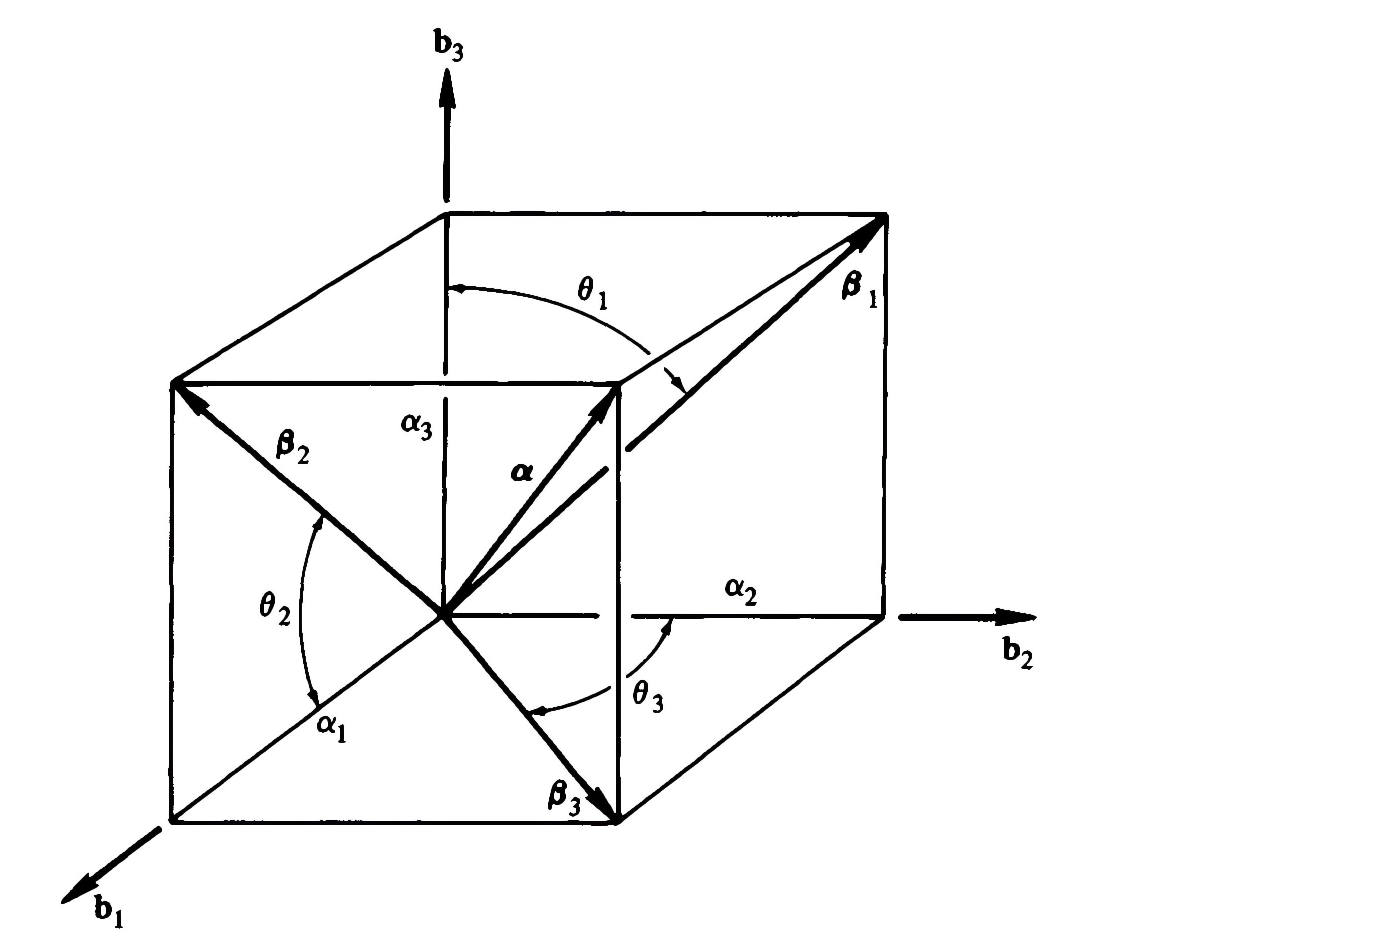
\includegraphics[width=0.8\textwidth]{Figure/角速度分量图1.png}
            \caption{角速度分量图1}
            \label{fig:角速度分量图1}
    \end{figure}
则 $\theta_1$（见图~\ref{fig:角速度分量图1}）可表示为
\begin{equation}
    \theta_1 = \tan^{-1}\frac{\alpha_2}{\alpha_3}
    \label{eq:角速度分量:theta1}
\end{equation}
由此可得
\begin{equation}
    \dot{\theta}_1 = \frac{\dot{\alpha}_2\alpha_3-\dot{\alpha}_3\alpha_2}{\alpha_2^2+\alpha_3^2}
    \label{eq:角速度分量:theta1导数}
\end{equation}
现在，$\dfrac{\mathrm{d}\bm{\alpha}}{\mathrm{d}t}\Big|_{B}$ 一方面可由
\begin{equation}
    \frac{\mathrm{d}\bm{\alpha}}{\mathrm{d}t}\Big|_{B} = \dot{\alpha}_1\mathbf{b}_1+\dot{\alpha}_2\mathbf{b}_2+\dot{\alpha}_3\mathbf{b}_3
    \label{eq:角速度分量:alpha导数A}
\end{equation}
给出，另一方面，由于 $\bm{\alpha}$ 固定于 $A$ 中，由式~\eqref{eq:角速度矢量:导数关系} 与式~\eqref{eq:角速度矢量:反对称性}，
\begin{equation}
    \frac{\mathrm{d}\bm{\alpha}}{\mathrm{d}t}\Big|_{B} = \bm{\omega}_{A|B}\times\bm{\alpha}
    = -\bm{\omega}_{B|A}\times\bm{\alpha}
    = (\alpha_2\omega_3-\alpha_3\omega_2)\mathbf{b}_1
    + (\alpha_3\omega_1-\alpha_1\omega_3)\mathbf{b}_2
    + (\alpha_1\omega_2-\alpha_2\omega_1)\mathbf{b}_3
    \label{eq:角速度分量:alpha导数B}
\end{equation}
于是，
\begin{equation}
    \dot{\alpha}_i = \eta_{ijk}(\alpha_j\omega_k-\alpha_k\omega_j) \quad (i=1,2,3)
    \label{eq:角速度分量:alpha导数}
\end{equation}
且
\begin{equation}
    \dot{\theta}_1 = \frac{(\alpha_3\omega_1-\alpha_1\omega_3)\alpha_3-(\alpha_1\omega_2-\alpha_2\omega_1)\alpha_2}{\alpha_2^2+\alpha_3^2}
    = \omega_1 - \frac{\alpha_1\alpha_2}{\alpha_2^2+\alpha_3^2}\,\omega_2 - \frac{\alpha_1\alpha_3}{\alpha_2^2+\alpha_3^2}\,\omega_3
    \label{eq:角速度分量:theta1展开}
\end{equation}

\begin{figure}[H]
    \centering
    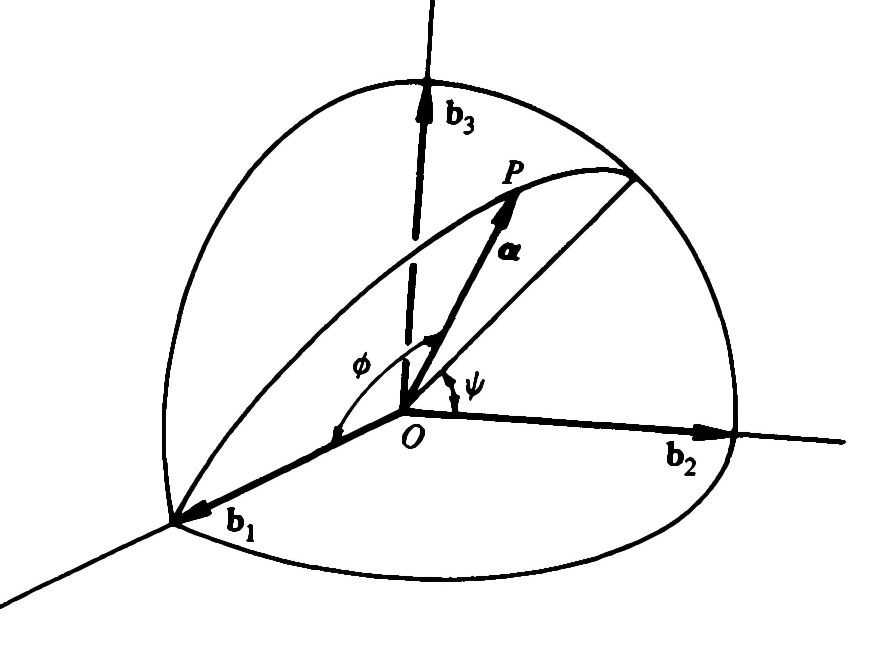
\includegraphics[width=0.8\textwidth]{Figure/角速度分量图2.png}
    \caption{角速度分量：单位球面上的 $\phi$ 与 $\psi$}
    \label{fig:角速度分量图2}
\end{figure}

为完成式~\eqref{eq:角速度分量:平均导数定义} 中的积分，引入图~\ref{fig:角速度分量图2} 中的角度 $\phi$ 与 $\psi$，此时 $\bm{\alpha}$ 可表示为
\begin{equation}
    \bm{\alpha} = \cos\phi\,\mathbf{b}_1 + \sin\phi\cos\psi\,\mathbf{b}_2 + \sin\phi\sin\psi\,\mathbf{b}_3
    \label{eq:角速度分量:alpha球面坐标}
\end{equation}
从而
\begin{equation}
    \alpha_1 = \cos\phi,\qquad \alpha_2 = \sin\phi\cos\psi,\qquad \alpha_3 = \sin\phi\sin\psi
    \label{eq:角速度分量:alpha分量}
\end{equation}
而
\begin{equation}
    \mathrm{d}\sigma = \sin\phi\,\mathrm{d}\phi\,\mathrm{d}\psi
    \label{eq:角速度分量:面积元}
\end{equation}
于是，
\begin{equation}
    \begin{aligned}
        4\pi\,\overline{\dot{\theta}}_1
        &= \omega_1\int_0^\pi\left[\int_0^{2\pi}\sin\phi\,\mathrm{d}\psi\right]\mathrm{d}\phi
        - \omega_2\int_0^\pi\left[\int_0^{2\pi}\cos\phi\cos\psi\,\mathrm{d}\psi\right]\mathrm{d}\phi\\
        &\quad - \omega_3\int_0^\pi\left[\int_0^{2\pi}\cos\phi\sin\psi\,\mathrm{d}\psi\right]\mathrm{d}\phi
    \end{aligned}
    \label{eq:角速度分量:积分}
\end{equation}
第一个二重积分的值为 $4\pi$，其余两个二重积分均为零。因此，
\begin{equation}
    \overline{\dot{\theta}}_1 = \omega_1
    \label{eq:角速度分量:theta1平均}
\end{equation}
类似地，
\begin{equation}
    \overline{\dot{\theta}}_2 = \omega_2,\qquad
    \overline{\dot{\theta}}_3 = \omega_3
    \label{eq:角速度分量:theta23平均}
\end{equation}

\end{proof}


\blocksep
\begin{example}
        \begin{figure}[H]
            \centering
            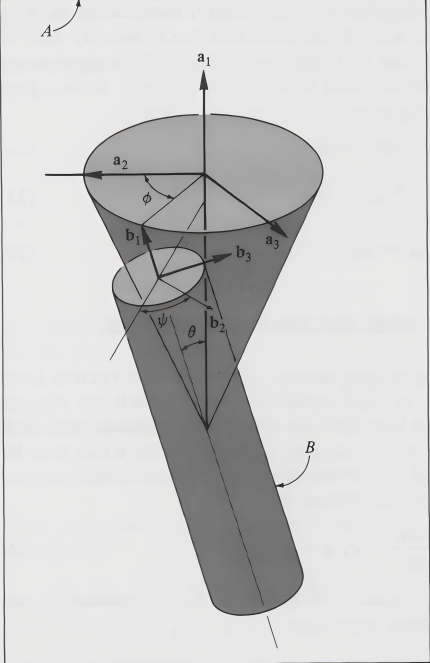
\includegraphics[width=0.8\textwidth]{Figure/角速度分量图3.png}
            \caption{角速度分量例题}
            \label{fig:角速度分量例题}
        \end{figure}
    在图~\ref{fig:角速度分量例题} 中，$B$ 表示一个圆柱形航天器，它在参考系 $A$ 中的姿态运动可以描述为锥运动（coning）与自旋（spinning）的组合：前者由角度 $\phi$ 刻画，涉及 $B$ 的对称轴在一个固定于 $A$、半顶角为常数 $\theta$ 的圆锥面上的运动；后者与角度 $\psi$ 的变化相联系，$\psi$ 是两条直线的夹角，这两条直线在 $B$ 的对称轴上相交并与之垂直，其中一条固定在 $B$ 中，另一条与圆锥的轴相交。在此情形下，满足
    \begin{equation}
        \begin{bmatrix}\mathbf{b}_1 & \mathbf{b}_2 & \mathbf{b}_3\end{bmatrix}
        = \begin{bmatrix}\mathbf{a}_1 & \mathbf{a}_2 & \mathbf{a}_3\end{bmatrix}\,\bm{A}
        \label{eq:角速度分量:圆锥DCM定义}
    \end{equation}
    的方向余弦矩阵 $\bm{A}$（其中 $\mathbf{a}_i$ 与 $\mathbf{b}_i$（$i=1,2,3$）为按图~\ref{fig:角速度分量例题} 所示方向取的单位向量）可表示为
    \begin{equation}
        \bm{A} = \bm{C}_1(\phi)\,\bm{C}_3(\theta)\,\bm{C}_1(\psi)
        \label{eq:角速度分量:DCM乘积}
    \end{equation}
    或按方向余弦矩阵计算式展开后写成
    \begin{equation}
        \bm{A} = \begin{bmatrix}
            c\theta & -s\theta\,c\psi & s\theta\,s\psi\\
            s\theta\,c\phi & c\theta\,c\phi\,c\psi-s\phi\,s\psi & -c\theta\,c\phi\,s\psi-s\phi\,c\psi\\
            s\theta\,s\phi & c\theta\,s\phi\,c\psi+c\phi\,s\psi & -c\theta\,s\phi\,s\psi+c\phi\,c\psi
        \end{bmatrix}
        \label{eq:角速度分量:DCM显式}
    \end{equation}
    其中 $s\theta$ 与 $c\theta$ 分别表示 $\sin\theta$ 与 $\cos\theta$，$\phi$、$\psi$ 同理。按照式~\eqref{eq:角速度矩阵:分量公式} 构成 $\omega_1,\omega_2,\omega_3$，即可得到 $B$ 在 $A$ 中的角速度 $\bm{\omega}$ 的如下表达式：
    \begin{equation}
        \bm{\omega} = (\dot{\psi}+\dot{\phi}\,c\theta)\,\mathbf{b}_1 - \dot{\phi}\,s\theta\,c\psi\,\mathbf{b}_2 + \dot{\phi}\,s\theta\,s\psi\,\mathbf{b}_3
        \label{eq:角速度分量:圆锥角速度}
    \end{equation}
    获得这一结果的更高效方法见第~\ref{sec:slow-small-rotation}~节。就本节的目的而言，值得注意的是 $\bm{\omega}$ 的 $\mathbf{b}_i$ 分量（$i=1,2,3$）并没有明显的物理意义；但当把 $\bm{\omega}$ 改写为
    \begin{equation}
        \bm{\omega} = \dot{\psi}\,\mathbf{b}_1 + \dot{\phi}(c\theta\,\mathbf{b}_1 - s\theta\,c\psi\,\mathbf{b}_2 + s\theta\,s\psi\,\mathbf{b}_3)
        \label{eq:角速度分量:分解}
    \end{equation}
    时，每个分量都具有式~\eqref{eq:角速度矢量:基本关系} 右端的形式，因而可视为一个作简单转动的物体的角速度。具体地，设 $A_1$ 为一个使圆锥的轴与 $B$ 的对称轴都固定的参考系，则 $A_1$ 在 $A$ 中作简单转动，$B$ 在 $A_1$ 中也作简单转动，相应的角速度分别为
    \begin{equation}
        \bm{\omega}_{A_1|A} = \dot{\phi}\,\mathbf{a}_1
        \label{eq:角速度分量:A1角速度}
    \end{equation}
    和
    \begin{equation}
        \bm{\omega}_{B|A_1} = \dot{\psi}\,\mathbf{b}_1
        \label{eq:角速度分量:B角速度}
    \end{equation}
    于是
    \begin{equation}
        \bm{\omega} = \bm{\omega}_{A_1|A} + \bm{\omega}_{B|A_1}
        \label{eq:角速度分量:角速度合成}
    \end{equation}
\end{example}
%=============================================================
\section{角速度与欧拉参数}
\begin{myTheorem}{角速度与欧拉参数的关系}
若 $\mathbf{a}_1,\mathbf{a}_2,\mathbf{a}_3$ 与 $\mathbf{b}_1,\mathbf{b}_2,\mathbf{b}_3$ 分别为固定在相互运动的参考系或刚体 $A$ 与 $B$ 中的两组成右手正交单位向量，则可以利用式~\eqref{eq:欧拉参数转方向余弦} 在每个时刻确定欧拉参数 $\epsilon_1,\dots,\epsilon_4$，并按式~\eqref{eq:欧拉参数定义} 构成欧拉向量 $\bm{\epsilon}$。用 $\bm{\epsilon}$ 和 $\epsilon_4$ 表示时，$B$ 在 $A$ 中的角速度（见角速度矢量一节）可以写成
\begin{equation}
    \bm{\omega} = 2\left(\epsilon_4\frac{\mathrm{d}\bm{\epsilon}}{\mathrm{d}t}\Big|_{B} - \dot{\epsilon}_4\bm{\epsilon} - \bm{\epsilon}\times\frac{\mathrm{d}\bm{\epsilon}}{\mathrm{d}t}\Big|_{B}\right)
    \label{eq:角速度欧拉:基本关系}
\end{equation}
反之，若 $\bm{\omega}$ 是已知的时间函数，则欧拉参数可以通过求解微分方程
\begin{equation}
    \frac{\mathrm{d}\bm{\epsilon}}{\mathrm{d}t}\Big|_{B} = \frac{1}{2}(\epsilon_4\bm{\omega} + \bm{\epsilon}\times\bm{\omega})
    \label{eq:角速度欧拉:微分方程}
\end{equation}
和
\begin{equation}
    \dot{\epsilon}_4 = -\frac{1}{2}\bm{\omega}\cdot\bm{\epsilon}
    \label{eq:角速度欧拉:epsilon4导数}
\end{equation}
得到。
\end{myTheorem}

与式~\eqref{eq:角速度欧拉:基本关系}--\eqref{eq:角速度欧拉:epsilon4导数} 等价的方程可以用增广列阵 $\bar{\bm{\omega}}$、$\bar{\bm{\epsilon}}$ 和矩阵 $E$ 表述。定义
\begin{equation}
    \bar{\bm{\omega}} \triangleq \begin{bmatrix}\omega_1\\\omega_2\\\omega_3\\0\end{bmatrix},\qquad
    \bar{\bm{\epsilon}} \triangleq \begin{bmatrix}\epsilon_1\\\epsilon_2\\\epsilon_3\\\epsilon_4\end{bmatrix}
    \label{eq:角速度欧拉:增广向量}
\end{equation}
以及
\begin{equation}
    E = \begin{bmatrix}
        \epsilon_4 & -\epsilon_3 & \epsilon_2 & \epsilon_1\\
        \epsilon_3 & \epsilon_4 & -\epsilon_1 & \epsilon_2\\
        -\epsilon_2 & \epsilon_1 & \epsilon_4 & \epsilon_3\\
        -\epsilon_1 & -\epsilon_2 & -\epsilon_3 & \epsilon_4
    \end{bmatrix}
    \label{eq:角速度欧拉:E矩阵}
\end{equation}
于是这些方程等价于
\begin{equation}
    \bar{\bm{\omega}} = 2E^{\mathrm{T}}\dot{\bar{\bm{\epsilon}}}
    \label{eq:角速度欧拉:矩阵形式1}
\end{equation}
和
\begin{equation}
    \dot{\bar{\bm{\epsilon}}} = \frac{1}{2}E\,\bar{\bm{\omega}}
    \label{eq:角速度欧拉:矩阵形式2}
\end{equation}

\begin{proof}
    将式~\eqref{eq:欧拉参数转方向余弦}（方向余弦的欧拉参数表示）代入式~\eqref{eq:角速度矩阵:分量公式}，得
\begin{equation}
    \begin{aligned}
        \omega_1 &= 4(\epsilon_3\epsilon_1+\epsilon_2\epsilon_4)(\dot{\epsilon}_1\epsilon_2+\epsilon_1\dot{\epsilon}_2-\dot{\epsilon}_3\epsilon_4-\epsilon_3\dot{\epsilon}_4)\\
        &\quad + 4(\epsilon_2\epsilon_3-\epsilon_1\epsilon_4)(\epsilon_2\dot{\epsilon}_2-\epsilon_3\dot{\epsilon}_3-\epsilon_1\dot{\epsilon}_1+\epsilon_4\dot{\epsilon}_4)\\
        &\quad + 2(1-2\epsilon_1^2-2\epsilon_2^2)(\dot{\epsilon}_2\epsilon_3+\epsilon_2\dot{\epsilon}_3+\dot{\epsilon}_1\epsilon_4+\epsilon_1\dot{\epsilon}_4)\\
        &= 2(\dot{\epsilon}_1\epsilon_4+\dot{\epsilon}_2\epsilon_3-\dot{\epsilon}_3\epsilon_2-\dot{\epsilon}_4\epsilon_1)
    \end{aligned}
    \label{eq:角速度欧拉:omega1推导}
\end{equation}
\begin{equation}
    \omega_2 = 2(\dot{\epsilon}_2\epsilon_4+\dot{\epsilon}_3\epsilon_1-\dot{\epsilon}_1\epsilon_3-\dot{\epsilon}_4\epsilon_2)
    \label{eq:角速度欧拉:omega2推导}
\end{equation}
\begin{equation}
    \omega_3 = 2(\dot{\epsilon}_3\epsilon_4+\dot{\epsilon}_1\epsilon_2-\dot{\epsilon}_2\epsilon_1-\dot{\epsilon}_4\epsilon_3)
    \label{eq:角速度欧拉:omega3推导}
\end{equation}
这三个方程正是与式~\eqref{eq:角速度欧拉:矩阵形式1} 对应的四个标量方程中的三个；第四个是
\begin{equation}
    0 = 2(\dot{\epsilon}_1\epsilon_1+\dot{\epsilon}_2\epsilon_2+\dot{\epsilon}_3\epsilon_3+\dot{\epsilon}_4\epsilon_4)
    \label{eq:角速度欧拉:第四方程}
\end{equation}
该方程自动成立，因为
\begin{equation}
    \dot{\epsilon}_1\epsilon_1+\dot{\epsilon}_2\epsilon_2+\dot{\epsilon}_3\epsilon_3+\dot{\epsilon}_4\epsilon_4
    = \frac{1}{2}\frac{\mathrm{d}}{\mathrm{d}t}(\epsilon_1^2+\epsilon_2^2+\epsilon_3^2+\epsilon_4^2)=0
\end{equation}
（由欧拉参数归一化条件式~\eqref{eq:欧拉参数归一化}）。于是式~\eqref{eq:角速度欧拉:矩阵形式1} 的成立得到验证；而式~\eqref{eq:角速度欧拉:基本关系} 可如下得出：
\begin{equation}
    \begin{aligned}
        \bm{\omega} &= \omega_1\mathbf{b}_1+\omega_2\mathbf{b}_2+\omega_3\mathbf{b}_3\\
        &= 2[\epsilon_4(\dot{\epsilon}_1\mathbf{b}_1+\dot{\epsilon}_2\mathbf{b}_2+\dot{\epsilon}_3\mathbf{b}_3) - \dot{\epsilon}_4(\epsilon_1\mathbf{b}_1+\epsilon_2\mathbf{b}_2+\epsilon_3\mathbf{b}_3)\\
        &\quad + (\dot{\epsilon}_2\epsilon_3-\dot{\epsilon}_3\epsilon_2)\mathbf{b}_1+(\dot{\epsilon}_3\epsilon_1-\dot{\epsilon}_1\epsilon_3)\mathbf{b}_2+(\dot{\epsilon}_1\epsilon_2-\dot{\epsilon}_2\epsilon_1)\mathbf{b}_3]\\
        &= 2\left(\epsilon_4\frac{\mathrm{d}\bm{\epsilon}}{\mathrm{d}t}\Big|_{B} - \dot{\epsilon}_4\bm{\epsilon} - \bm{\epsilon}\times\frac{\mathrm{d}\bm{\epsilon}}{\mathrm{d}t}\Big|_{B}\right)
    \end{aligned}
    \label{eq:角速度欧拉:omega推导}
\end{equation}

将式~\eqref{eq:角速度欧拉:矩阵形式1} 两端左乘 $E$，并利用 $EE^{\mathrm{T}}=\bm{I}$（可由式~\eqref{eq:欧拉参数归一化} 验证），得
\begin{equation}
    E\,\bar{\bm{\omega}} = 2E\,E^{\mathrm{T}}\dot{\bar{\bm{\epsilon}}} = 2\dot{\bar{\bm{\epsilon}}}
\end{equation}
即
\begin{equation}
    \dot{\bar{\bm{\epsilon}}} = \frac{1}{2}E\,\bar{\bm{\omega}}
\end{equation}
与式~\eqref{eq:角速度欧拉:矩阵形式2} 一致。

最后，
\begin{equation}
    \dot{\epsilon}_4 = -\frac{1}{2}(\omega_1\epsilon_1+\omega_2\epsilon_2+\omega_3\epsilon_3) = -\frac{1}{2}\bm{\omega}\cdot\bm{\epsilon}
    \label{eq:角速度欧拉:epsilon4推导}
\end{equation}
如式~\eqref{eq:角速度欧拉:epsilon4导数} 所示；并且
\begin{equation}
    \frac{\mathrm{d}\bm{\epsilon}}{\mathrm{d}t}\Big|_{B} = \dot{\epsilon}_1\mathbf{b}_1+\dot{\epsilon}_2\mathbf{b}_2+\dot{\epsilon}_3\mathbf{b}_3
    = \frac{1}{2}\left[(\omega_1\epsilon_4-\omega_2\epsilon_3+\omega_3\epsilon_2)\mathbf{b}_1
    + (\omega_1\epsilon_3+\omega_2\epsilon_4-\omega_3\epsilon_1)\mathbf{b}_2
    - (\omega_1\epsilon_2-\omega_2\epsilon_1-\omega_3\epsilon_4)\mathbf{b}_3\right]
    \label{eq:角速度欧拉:epsilon导数推导}
\end{equation}
其右端与式~\eqref{eq:角速度欧拉:微分方程} 的右端相等。

\end{proof}

\blocksep
\begin{example}
    设 $B$ 关于其质心 $B^*$ 的惯性椭球为回转椭球，其回转轴平行于 $\mathbf{b}_1$。若 $\mathbf{I}$ 表示 $B$ 关于 $B^*$ 的惯性并矢，并定义 $I$ 与 $J$ 为
    \begin{equation}
        I\triangleq\mathbf{b}_1\cdot\mathbf{I}\cdot\mathbf{b}_1=\mathbf{b}_2\cdot\mathbf{I}\cdot\mathbf{b}_2
        \label{eq:角速度欧拉:惯性矩I}
    \end{equation}
    和
    \begin{equation}
        J\triangleq\mathbf{b}_3\cdot\mathbf{I}\cdot\mathbf{b}_3
        \label{eq:角速度欧拉:惯性矩J}
    \end{equation}
    则 $B$ 在 $A$ 中关于 $B^*$ 的角动量 $\mathbf{H}$ 为
    \begin{equation}
        \mathbf{H}=I\omega_1\mathbf{b}_1+I\omega_2\mathbf{b}_2+J\omega_3\mathbf{b}_3
        \label{eq:角速度欧拉:角动量}
    \end{equation}
    且 $\mathbf{H}$ 在 $A$ 中的一阶时间导数可表示为（见式~\eqref{eq:角速度矢量:导数关系}）
    \begin{equation}
        \begin{aligned}
            \frac{\mathrm{d}\mathbf{H}}{\mathrm{d}t}\Big|_{A} &= \frac{\mathrm{d}\mathbf{H}}{\mathrm{d}t}\Big|_{B} + \bm{\omega}\times\mathbf{H}\\
            &= [I\dot{\omega}_1+(J-I)\omega_2\omega_3]\mathbf{b}_1
            + [I\dot{\omega}_2-(J-I)\omega_3\omega_1]\mathbf{b}_2
            + J\dot{\omega}_3\mathbf{b}_3
        \end{aligned}
        \label{eq:角速度欧拉:角动量导数}
    \end{equation}
    因此，若 $B$ 在合力作用下运动，且这些力对 $B^*$ 的力矩之和为零，$A$ 为惯性参考系，则按角动量定理，$\mathbf{H}$ 在 $A$ 中的时间导数为零，于是 $\omega_1,\omega_2,\omega_3$ 满足微分方程
    \begin{equation}
        \dot{\omega}_1 - \frac{I-J}{I}\,\omega_2\omega_3 = 0
    \end{equation}
    \begin{equation}
        \dot{\omega}_2 + \frac{I-J}{I}\,\omega_3\omega_1 = 0
    \end{equation}
    \begin{equation}
        \dot{\omega}_3 = 0
    \end{equation}
    设 $\overline{\omega}_i$ 表示 $\omega_i$（$i=1,2,3$）在 $t=0$ 时的值，并定义常数 $s$ 为
    \begin{equation}
        s \triangleq \frac{I-J}{I}\,\omega_3
        \label{eq:角速度欧拉:常数s}
    \end{equation}
    则上述微分方程的通解可以表示为
    \begin{equation}
        \omega_1 = \overline{\omega}_1\cos st + \overline{\omega}_2\sin st
    \end{equation}
    \begin{equation}
        \omega_2 = -\overline{\omega}_1\sin st + \overline{\omega}_2\cos st
    \end{equation}
    \begin{equation}
        \omega_3 = \overline{\omega}_3
    \end{equation}
    为确定 $B$ 在 $A$ 中的姿态，还需求解微分方程
    \begin{equation}
        \dot{\epsilon}_1 = \frac{1}{2}(\omega_1\epsilon_4-\omega_2\epsilon_3+\omega_3\epsilon_2)
        = \frac{1}{2}[(\overline{\omega}_1\cos st+\overline{\omega}_2\sin st)\epsilon_4
        + (\overline{\omega}_1\sin st-\overline{\omega}_2\cos st)\epsilon_3
        + \overline{\omega}_3\epsilon_2]
    \end{equation}
    \begin{equation}
        \dot{\epsilon}_2 = \frac{1}{2}(\omega_1\epsilon_3+\omega_2\epsilon_4-\omega_3\epsilon_1)
        = \frac{1}{2}[(\overline{\omega}_1\cos st+\overline{\omega}_2\sin st)\epsilon_3
        - (\overline{\omega}_1\sin st-\overline{\omega}_2\cos st)\epsilon_4
        - \overline{\omega}_3\epsilon_1]
    \end{equation}
    \begin{equation}
        \dot{\epsilon}_3 = \frac{1}{2}(-\omega_1\epsilon_2+\omega_2\epsilon_1+\omega_3\epsilon_4)
        = \frac{1}{2}[-(\overline{\omega}_1\cos st+\overline{\omega}_2\sin st)\epsilon_2
        + (-\overline{\omega}_1\sin st+\overline{\omega}_2\cos st)\epsilon_1
        + \overline{\omega}_3\epsilon_4]
    \end{equation}
    \begin{equation}
        \dot{\epsilon}_4 = -\frac{1}{2}(\omega_1\epsilon_1+\omega_2\epsilon_2+\omega_3\epsilon_3)
        = -\frac{1}{2}[(\overline{\omega}_1\cos st+\overline{\omega}_2\sin st)\epsilon_1
        + (-\overline{\omega}_1\sin st+\overline{\omega}_2\cos st)\epsilon_2
        + \overline{\omega}_3\epsilon_3]
    \end{equation}
    初始条件取为
    \begin{equation}
        \epsilon_1=\epsilon_2=\epsilon_3=0,\qquad \epsilon_4=1\quad (t=0)
    \end{equation}
    这意味着在 $t=0$ 时选单位向量 $\mathbf{a}_1,\mathbf{a}_2,\mathbf{a}_3$ 使 $\mathbf{a}_i=\mathbf{b}_i$（$i=1,2,3$）。由于上述方程具有随时间变化的系数，无法用简单的解析方法求解 $\epsilon_1,\dots,\epsilon_4$。不过，换一种方法处理手头的物理问题（见第~\ref{sec:direction-cosines}~节），并定义量 $p$ 为
    \begin{equation}
        p \triangleq \left[\overline{\omega}_1^2+\overline{\omega}_2^2+\left(\frac{J}{I}\overline{\omega}_3\right)^2\right]^{1/2}
        \label{eq:角速度欧拉:常数p}
    \end{equation}
    则 $\epsilon_1,\epsilon_2,\epsilon_3,\epsilon_4$ 可表示为
    \begin{equation}
        \epsilon_1 = \frac{\sin(pt/2)}{p}\left(\overline{\omega}_1\cos\frac{st}{2}+\overline{\omega}_2\sin\frac{st}{2}\right)
    \end{equation}
    \begin{equation}
        \epsilon_2 = \frac{\sin(pt/2)}{p}\left(-\overline{\omega}_1\sin\frac{st}{2}+\overline{\omega}_2\cos\frac{st}{2}\right)
    \end{equation}
    \begin{equation}
        \epsilon_3 = \overline{\omega}_3\frac{J}{Ip}\sin\frac{pt}{2}\cos\frac{st}{2}+\cos\frac{pt}{2}\sin\frac{st}{2}
    \end{equation}
    \begin{equation}
        \epsilon_4 = -\overline{\omega}_3\frac{J}{Ip}\sin\frac{pt}{2}\sin\frac{st}{2}+\cos\frac{pt}{2}\cos\frac{st}{2}
    \end{equation}
    可以验证，这些表达式确实满足上述微分方程。
\end{example}

%=============================================================
\section{辅助参考系}
\begin{myTheorem}{角速度加法定理}
刚体 $B$ 在参考系 $A$ 中的角速度（见角速度矢量一节）可以用涉及 $n$ 个辅助参考系 $A_1,\dots,A_n$ 的如下形式表达：
\begin{equation}
    \bm{\omega}_{B|A} = \bm{\omega}_{A_1|A} + \bm{\omega}_{A_2|A_1} + \cdots + \bm{\omega}_{A_n|A_{n-1}} + \bm{\omega}_{B|A_n}
    \label{eq:辅助参考系:角速度加法定理}
\end{equation}
这个关系称为角速度加法定理，当右端每一项都表示一个作简单转动（见简单转动一节）的物体的角速度（从而可按式~\eqref{eq:角速度矢量:基本关系} 表达）时特别有用。
\end{myTheorem}

\begin{proof}
    对任何固定在 $B$ 中的向量 $\mathbf{c}$，由式~\eqref{eq:角速度矢量:导数关系}，
\begin{equation}
    \frac{\mathrm{d}\mathbf{c}}{\mathrm{d}t}\Big|_{A} = \bm{\omega}_{B|A}\times\mathbf{c}
\end{equation}
\begin{equation}
    \frac{\mathrm{d}\mathbf{c}}{\mathrm{d}t}\Big|_{A_1} = \bm{\omega}_{B|A_1}\times\mathbf{c}
\end{equation}
以及
\begin{equation}
    \frac{\mathrm{d}\mathbf{c}}{\mathrm{d}t}\Big|_{A} = \frac{\mathrm{d}\mathbf{c}}{\mathrm{d}t}\Big|_{A_1} + \bm{\omega}_{A_1|A}\times\mathbf{c}
\end{equation}
从而
\begin{equation}
    \bm{\omega}_{B|A}\times\mathbf{c} = \bm{\omega}_{A_1|A}\times\mathbf{c} + \bm{\omega}_{B|A_1}\times\mathbf{c}
\end{equation}
由于该式对每个固定在 $B$ 中的 $\mathbf{c}$ 均成立，
\begin{equation}
    \bm{\omega}_{B|A} = \bm{\omega}_{A_1|A} + \bm{\omega}_{B|A_1}
    \label{eq:辅助参考系:n=1}
\end{equation}
这说明式~\eqref{eq:辅助参考系:角速度加法定理} 对 $n=1$ 成立。类似地可以验证
\begin{equation}
    \bm{\omega}_{B|A_1} = \bm{\omega}_{A_2|A_1} + \bm{\omega}_{B|A_2}
\end{equation}
将其代入式~\eqref{eq:辅助参考系:n=1}，得
\begin{equation}
    \bm{\omega}_{B|A} = \bm{\omega}_{A_1|A} + \bm{\omega}_{A_2|A_1} + \bm{\omega}_{B|A_2}
    \label{eq:辅助参考系:n=2}
\end{equation}
即式~\eqref{eq:辅助参考系:角速度加法定理} 对 $n=2$ 成立。对任意 $n$，把这一过程重复足够多次即可验证式~\eqref{eq:辅助参考系:角速度加法定理} 成立。

\end{proof}

\blocksep
\begin{example}
    在图~\ref{fig:缓慢小转动例题} 中，$\theta,\phi,\psi$ 表示用于描述刚体圆锥 $B$ 在参考系 $A$ 中姿态的角度。这些角度由如下直线构成：$L_1$ 与 $L_2$ 相互垂直且固定在 $A$ 中；$L_3$ 是 $B$ 的对称轴；$L_4$ 垂直于 $L_2$ 并与 $L_2$、$L_3$ 相交；$L_5$ 垂直于 $L_3$ 并与 $L_2$、$L_3$ 相交；$L_6$ 垂直于 $L_3$ 且固定在 $B$ 中；$L_7$ 垂直于 $L_2$ 与 $L_4$。为求 $B$ 在 $A$ 中的角速度，可以取 $A_1$ 为使 $L_2,L_4,L_7$ 固定的参考系，取 $A_2$ 为使 $L_3,L_5,L_7$ 固定的参考系，并注意到 $L_2$ 同时固定在 $A$ 与 $A_1$ 中，$L_7$ 同时固定在 $A_1$ 与 $A_2$ 中，$L_3$ 同时固定在 $A_2$ 与 $B$ 中。于是按式~\eqref{eq:角速度矢量:基本关系}，
    \begin{equation}
        \bm{\omega}_{A_1|A} = \dot{\phi}\,\bm{\lambda}_2,\qquad
        \bm{\omega}_{A_2|A_1} = \dot{\theta}\,\bm{\lambda}_7,\qquad
        \bm{\omega}_{B|A_2} = \dot{\psi}\,\bm{\lambda}_3
        \label{eq:辅助参考系:各角速度}
    \end{equation}
    其中 $\bm{\lambda}_2,\bm{\lambda}_3,\bm{\lambda}_7$ 为按图~\ref{fig:缓慢小转动例题} 所示方向取的单位向量。于是立即得到
    \begin{equation}
        \bm{\omega}_{B|A} = \dot{\phi}\,\bm{\lambda}_2 + \dot{\theta}\,\bm{\lambda}_7 + \dot{\psi}\,\bm{\lambda}_3
        \label{eq:辅助参考系:角速度合成}
    \end{equation}
\end{example}

%=============================================================
\section{角速度与方向角}
\begin{myTheorem}{角速度与方向角的关系}
当刚体 $B$ 在参考系 $A$ 中的姿态用方向角 $\theta_1,\theta_2,\theta_3$（见方向角一节）的时间依赖关系描述时，$B$ 在 $A$ 中的角速度（见角速度矢量一节）可以通过如下关系求出：
\begin{equation}
    \begin{bmatrix}\omega_1 & \omega_2 & \omega_3\end{bmatrix}
    = \begin{bmatrix}\dot{\theta}_1 & \dot{\theta}_2 & \dot{\theta}_3\end{bmatrix}\,\bm{M}
    \label{eq:方向角角速度:基本关系}
\end{equation}
其中 $\bm{M}$ 是一个 $3\times3$ 矩阵，其元素为 $\theta_1,\theta_2,\theta_3$ 的函数。反之，若 $\omega_1,\omega_2,\omega_3$ 是已知的时间函数，则 $\theta_1,\theta_2,\theta_3$ 可以通过求解微分方程
\begin{equation}
    \begin{bmatrix}\dot{\theta}_1 & \dot{\theta}_2 & \dot{\theta}_3\end{bmatrix}
    = \begin{bmatrix}\omega_1 & \omega_2 & \omega_3\end{bmatrix}\,\bm{M}^{-1}
    \label{eq:方向角角速度:逆关系}
\end{equation}
求得。
\end{myTheorem}

对于空间三转角（space-three angles），矩阵 $\bm{M}$ 与 $\bm{M}^{-1}$ 为
\begin{equation}
    \bm{M} = \begin{bmatrix}
        1 & 0 & 0\\
        0 & c_1 & -s_1\\
        -s_2 & s_1c_2 & c_1c_2
    \end{bmatrix},\qquad
    \bm{M}^{-1} = \frac{1}{c_2}\begin{bmatrix}
        c_2 & 0 & 0\\
        s_1s_2 & c_1c_2 & s_1\\
        c_1s_2 & -s_1c_2 & c_1
    \end{bmatrix}
    \label{eq:方向角角速度:空间三转角}
\end{equation}
对于体三转角（body-three angles），
\begin{equation}
    \bm{M} = \begin{bmatrix}
        c_2c_3 & -c_2s_3 & s_2\\
        s_3 & c_3 & 0\\
        0 & 0 & 1
    \end{bmatrix},\qquad
    \bm{M}^{-1} = \frac{1}{c_2}\begin{bmatrix}
        c_3 & c_2s_3 & -s_2c_3\\
        -s_3 & c_2c_3 & s_2s_3\\
        0 & 0 & c_2
    \end{bmatrix}
    \label{eq:方向角角速度:体三转角}
\end{equation}
对于空间二转角（space-two angles），
\begin{equation}
    \bm{M} = \begin{bmatrix}
        1 & 0 & 0\\
        0 & c_1 & -s_1\\
        c_2 & s_1s_2 & c_1s_2
    \end{bmatrix},\qquad
    \bm{M}^{-1} = \frac{1}{s_2}\begin{bmatrix}
        s_2 & 0 & 0\\
        -s_1c_2 & c_1s_2 & s_1\\
        -c_1c_2 & -s_1s_2 & c_1
    \end{bmatrix}
    \label{eq:方向角角速度:空间二转角}
\end{equation}
最后，对于体二转角（body-two angles），
\begin{equation}
    \bm{M} = \begin{bmatrix}
        c_2 & s_2s_3 & s_2c_3\\
        0 & c_3 & -s_3\\
        1 & 0 & 0
    \end{bmatrix},\qquad
    \bm{M}^{-1} = \frac{1}{s_2}\begin{bmatrix}
        0 & 0 & s_2\\
        s_3 & s_2c_3 & -c_2s_3\\
        c_3 & -s_2s_3 & -c_2c_3
    \end{bmatrix}
    \label{eq:方向角角速度:体二转角}
\end{equation}
当 $c_2$ 为零时，式~\eqref{eq:方向角角速度:空间三转角} 或式~\eqref{eq:方向角角速度:体三转角} 给出的 $\bm{M}$ 为奇异矩阵，$\bm{M}^{-1}$ 无定义。因此，给定 $\omega_1,\omega_2,\omega_3$ 后，若 $\theta_1,\theta_2,\theta_3$ 为空间三转角或体三转角且 $c_2=0$，则不能用式~\eqref{eq:方向角角速度:逆关系} 确定 $\dot{\theta}_1,\dot{\theta}_2,\dot{\theta}_3$。类似地，若 $\theta_1,\theta_2,\theta_3$ 为空间二转角或体二转角，则当 $s_2$ 为零时式~\eqref{eq:方向角角速度:逆关系} 涉及无定义的矩阵。

当分析中所用角度与单位向量的记号与式~\eqref{eq:方向角角速度:基本关系}--\eqref{eq:方向角角速度:体二转角} 不同时，只要确定了角度类型（空间三转角、体三转角等），就可以直接从式~\eqref{eq:方向角角速度:基本关系}--\eqref{eq:方向角角速度:体二转角} 得到相应的替换关系。例如，设在涉及图~\ref{fig:缓慢小转动例题} 中圆锥的分析中（该圆锥在第~\ref{sec:slow-small-rotation}~节例题中已讨论过），引入了固定在 $B$ 中的单位向量 $\mathbf{b}_x,\mathbf{b}_y,\mathbf{b}_z$（如图~\ref{fig:角速度与方向角} 所示），并希望求出
\begin{equation}
    \omega_x \triangleq \bm{\omega}\cdot\mathbf{b}_x,\qquad
    \omega_y \triangleq \bm{\omega}\cdot\mathbf{b}_y,\qquad
    \omega_z \triangleq \bm{\omega}\cdot\mathbf{b}_z
    \label{eq:方向角角速度:omega_xyz}
\end{equation}
\begin{figure}[H]
    \centering
    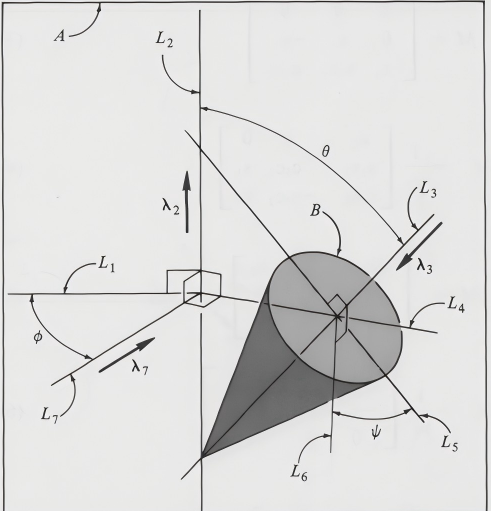
\includegraphics[width=0.8\textwidth]{Figure/角速度与方向角图.png}
    \caption{角速度与方向角：圆锥与单位向量}
    \label{fig:角速度与方向角}
\end{figure}

其中 $\bm{\omega}$ 表示 $B$ 在 $A$ 中的角速度。这可以通过把 $\phi,\theta,\psi$ 视为体二转角、并按图~\ref{fig:角速度与方向角} 所示引入单位向量 $\mathbf{a}_1,\mathbf{a}_2,\mathbf{a}_3$ 来完成，即定义
\begin{equation}
    \mathbf{b}_1 \triangleq \mathbf{b}_y,\qquad
    \mathbf{b}_2 \triangleq \mathbf{b}_z,\qquad
    \mathbf{b}_3 \triangleq \mathbf{b}_x
    \label{eq:方向角角速度:置换}
\end{equation}
并取
\begin{equation}
    \theta_1 = \phi,\qquad \theta_2 = -\theta,\qquad \theta_3 = -\psi
    \label{eq:方向角角速度:角度对应}
\end{equation}
由式~\eqref{eq:方向角角速度:基本关系} 和式~\eqref{eq:方向角角速度:体二转角} 立即可得
\begin{equation}
    \begin{bmatrix}\omega_y & \omega_z & \omega_x\end{bmatrix}
    = \begin{bmatrix}\dot{\phi} & -\dot{\theta} & -\dot{\psi}\end{bmatrix}
    \begin{bmatrix}
        \cos\theta & \sin\theta\sin\psi & -\sin\theta\cos\psi\\
        0 & \cos\psi & \sin\psi\\
        1 & 0 & 0
    \end{bmatrix}
    \label{eq:方向角角速度:圆锥关系}
\end{equation}
于是
\begin{equation}
    \omega_x = -\dot{\phi}\sin\theta\cos\psi - \dot{\theta}\sin\psi
\end{equation}
\begin{equation}
    \omega_y = \dot{\phi}\cos\theta - \dot{\psi}
\end{equation}
\begin{equation}
    \omega_z = \dot{\phi}\sin\theta\sin\psi - \dot{\theta}\cos\psi
\end{equation}
在航天器动力学文献中可以见到大量把角速度测度数（measure numbers）与方向角及其时间导数联系起来的微分方程。Kane《Spacecraft Dynamics》一书附录 II 中列出了 24 组这样的运动学微分方程。

\begin{proof}
    由式~\eqref{eq:角速度矩阵:分量公式} 和空间三转角的方向余弦矩阵公式，
\begin{equation}
    \omega_1 = (c_1s_2c_3+s_3s_1)\frac{\mathrm{d}}{\mathrm{d}t}(s_1s_2c_3-s_3c_1)
    + (c_1s_2s_3-c_3s_1)\frac{\mathrm{d}}{\mathrm{d}t}(s_1s_2s_3+c_3c_1)
    + c_1c_2\frac{\mathrm{d}}{\mathrm{d}t}(s_1c_2) = \dot{\theta}_1-\dot{\theta}_3s_2
\end{equation}
类似地，由式~\eqref{eq:角速度矩阵:分量公式} 可得
\begin{equation}
    \omega_2 = \dot{\theta}_2c_1+\dot{\theta}_3s_1c_2
\end{equation}
和
\begin{equation}
    \omega_3 = -\dot{\theta}_2s_1+\dot{\theta}_3c_1c_2
\end{equation}
当 $\bm{M}$ 由式~\eqref{eq:方向角角速度:空间三转角} 给出时，这三个方程正是与式~\eqref{eq:方向角角速度:基本关系} 对应的三个标量方程。

式~\eqref{eq:方向角角速度:逆关系} 可由式~\eqref{eq:方向角角速度:基本关系} 及逆矩阵的定义得出；式~\eqref{eq:方向角角速度:空间三转角} 的第二个等式的有效性可通过验证式~\eqref{eq:方向角角速度:空间三转角} 中两个矩阵右端的乘积等于单位阵 $\bm{I}$ 来确立。类似地，把式~\eqref{eq:方向角角速度:空间三转角}--\eqref{eq:方向角角速度:体二转角} 中的第一组换成第二组、第三组或第四组，即可验证其余各式的有效性。

\end{proof}

\blocksep
\begin{example}
        \begin{figure}[H]
            \centering
            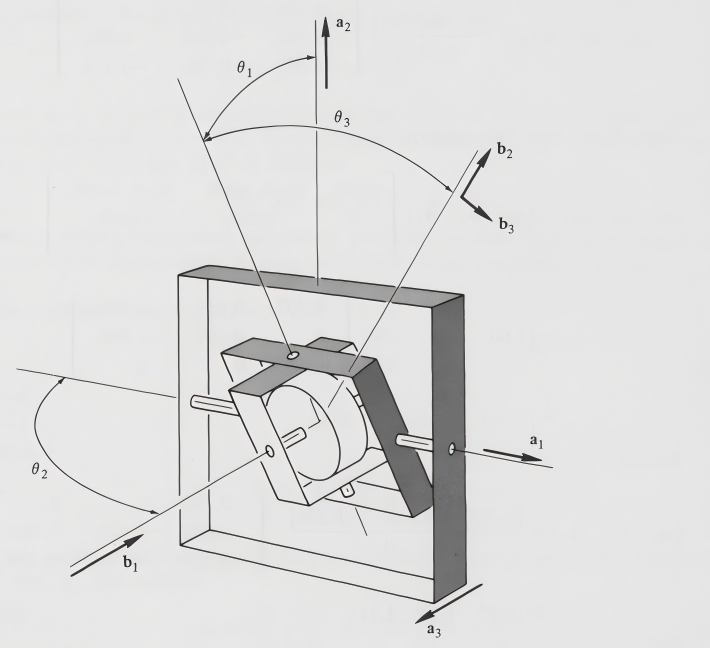
\includegraphics[width=0.8\textwidth]{Figure/角速度和方向角图2.png}
            \caption{角速度与方向角例题（陀螺系统）}
            \label{fig:角速度与方向角例题}
        \end{figure}
    图~\ref{fig:角速度与方向角例题} 所示即第~\ref{sec:euler-angles}~节讨论过的陀螺系统，那里提到，在分析 $\theta_2$ 变小时宜同时采用空间三转角 $\phi_1,\phi_2,\phi_3$ 与图~\ref{fig:角速度与方向角例题} 所示的体二转角 $\theta_1,\theta_2,\theta_3$。给定 $\theta_i$ 与 $\dot{\theta}_i$（$i=1,2,3$），就需要能够求出 $\phi_i$ 与 $\dot{\phi}_i$（$i=1,2,3$）。设如第~\ref{sec:euler-angles}~节例题那样，在某瞬时 $\theta_1=30^\circ$、$\theta_2=45^\circ$、$\theta_3=60^\circ$，且 $\dot{\theta}_1=1.00$、$\dot{\theta}_2=2.00$、$\dot{\theta}_3=3.00$ rad/s。求该瞬时 $\dot{\phi}_1,\dot{\phi}_2,\dot{\phi}_3$ 的值。由式~\eqref{eq:方向角角速度:逆关系} 和式~\eqref{eq:方向角角速度:空间三转角}，
    \begin{equation}
        \begin{bmatrix}\dot{\phi}_1 & \dot{\phi}_2 & \dot{\phi}_3\end{bmatrix}
        = \frac{\begin{bmatrix}\omega_1 & \omega_2 & \omega_3\end{bmatrix}}{\cos\phi_2}
        \begin{bmatrix}
            \cos\phi_2 & 0 & 0\\
            \sin\phi_1\sin\phi_2 & \cos\phi_1\cos\phi_2 & \sin\phi_1\\
            \cos\phi_1\sin\phi_2 & -\sin\phi_1\cos\phi_2 & \cos\phi_1
        \end{bmatrix}
    \end{equation}
    利用先前求得的 $\phi_1$ 与 $\phi_2$ 的数值，
    \begin{equation}
        \begin{bmatrix}\dot{\phi}_1 & \dot{\phi}_2 & \dot{\phi}_3\end{bmatrix}
        = \frac{\begin{bmatrix}\omega_1 & \omega_2 & \omega_3\end{bmatrix}}{0.791}
        \begin{bmatrix}
            0.791 & 0 & 0\\
            0.603 & -0.138 & 0.985\\
            -0.107 & -0.780 & -0.174
        \end{bmatrix}
    \end{equation}
    现在，由式~\eqref{eq:方向角角速度:基本关系} 和式~\eqref{eq:方向角角速度:体二转角}，
    \begin{equation}
        \begin{bmatrix}\omega_1 & \omega_2 & \omega_3\end{bmatrix}
        = \begin{bmatrix}\dot{\theta}_1 & \dot{\theta}_2 & \dot{\theta}_3\end{bmatrix}
        \begin{bmatrix}
            \cos\theta_2 & \sin\theta_2\sin\theta_3 & \sin\theta_2\cos\theta_3\\
            0 & \cos\theta_3 & -\sin\theta_3\\
            1 & 0 & 0
        \end{bmatrix}
        = \begin{bmatrix}1.00 & 2.00 & 3.00\end{bmatrix}
        \begin{bmatrix}
            0.707 & 0.612 & 0.354\\
            0 & 0.500 & -0.866\\
            1 & 0 & 0
        \end{bmatrix}
        = \begin{bmatrix}3.707 & 1.612 & -1.378\end{bmatrix}
    \end{equation}
    于是
    \begin{equation}
        \begin{bmatrix}\dot{\phi}_1 & \dot{\phi}_2 & \dot{\phi}_3\end{bmatrix}
        = \frac{\begin{bmatrix}3.707 & 1.612 & -1.378\end{bmatrix}}{0.791}
        \begin{bmatrix}
            0.791 & 0 & 0\\
            0.603 & -0.138 & 0.985\\
            -0.107 & -0.780 & -0.174
        \end{bmatrix}
        = \begin{bmatrix}5.12 & 1.08 & 2.31\end{bmatrix}
    \end{equation}
    即 $\dot{\phi}_1=5.12$、$\dot{\phi}_2=1.08$、$\dot{\phi}_3=2.31$ rad/s。
\end{example}

%=============================================================
\section{缓慢小转动}\label{sec:slow-small-rotation}
\begin{myTheorem}{缓慢小转动的简化关系}
若 $\mathbf{a}_1,\mathbf{a}_2,\mathbf{a}_3$ 与 $\mathbf{b}_1,\mathbf{b}_2,\mathbf{b}_3$ 分别为固定在相互运动的参考系或刚体 $A$ 与 $B$ 中的两组成右手正交单位向量，则可利用式~\eqref{eq:欧拉参数转方向余弦} 在每个时刻确定一个角度 $\theta$。当 $\theta$ 与 $\dot{\theta}$ 的二次及二次以上各项在运动分析中所起的作用可以忽略时，称该运动为缓慢小转动（slow, small rotational motion）。在这种情况下，前述许多关系可以换成更简单的形式。具体地，式~\eqref{eq:角速度欧拉:基本关系} 和式~\eqref{eq:角速度欧拉:epsilon4导数} 可分别换成
\begin{equation}
    \bm{\omega} = 2\frac{\mathrm{d}\bm{\epsilon}}{\mathrm{d}t}\Big|_{B}
    \label{eq:缓慢小转动:omega}
\end{equation}
和
\begin{equation}
    \epsilon_4 = 1
    \label{eq:缓慢小转动:epsilon4}
\end{equation}
而式~\eqref{eq:角速度欧拉:微分方程} 和式~\eqref{eq:角速度欧拉:基本关系} 又可换成
\begin{equation}
    \bm{\omega} = 2\frac{\mathrm{d}\bm{p}}{\mathrm{d}t}\Big|_{B}
    \label{eq:缓慢小转动:omega_p}
\end{equation}
此外，若选取 $\theta_1,\theta_2,\theta_3$ 使 $\theta_i$ 和/或 $\theta_j$（$i,j=1,2,3$）的二次及二次以上各项可以忽略，则式~\eqref{eq:方向角角速度:基本关系} 结合式~\eqref{eq:方向角角速度:空间三转角} 或式~\eqref{eq:方向角角速度:体三转角} 可得
\begin{equation}
    \begin{bmatrix}\omega_1 & \omega_2 & \omega_3\end{bmatrix}
    = \begin{bmatrix}\dot{\theta}_1 & \dot{\theta}_2 & \dot{\theta}_3\end{bmatrix}
    \label{eq:缓慢小转动:方向角}
\end{equation}
这说明在缓慢小转动中，使用空间三转角还是体三转角并无区别。
\end{myTheorem}

\begin{proof}
    由欧拉参数的定义（式~\eqref{eq:欧拉参数定义}），
\begin{equation}
    \bm{\epsilon} = \frac{1}{2}\bm{\lambda}\theta
\end{equation}
和
\begin{equation}
    \epsilon_4 = 1
\end{equation}
于是
\begin{equation}
    \frac{\mathrm{d}\bm{\epsilon}}{\mathrm{d}t}\Big|_{B} = \frac{1}{2}\left(\frac{\mathrm{d}\bm{\lambda}}{\mathrm{d}t}\Big|_{B}\theta + \bm{\lambda}\dot{\theta}\right)
\end{equation}
代入式~\eqref{eq:角速度欧拉:基本关系}，并只保留 $\theta$ 与 $\dot{\theta}$ 的一次项，得
\begin{equation}
    \bm{\omega} = 2\left[\frac{1}{2}\left(\frac{\mathrm{d}\bm{\lambda}}{\mathrm{d}t}\Big|_{B}\theta + \bm{\lambda}\dot{\theta}\right)\right] = 2\frac{\mathrm{d}\bm{\epsilon}}{\mathrm{d}t}\Big|_{B}
\end{equation}
与式~\eqref{eq:缓慢小转动:omega} 一致。式~\eqref{eq:缓慢小转动:epsilon4} 与 $\epsilon_4=\cos\frac{\theta}{2}$ 相同。

式~\eqref{eq:缓慢小转动:omega_p} 由式~\eqref{eq:缓慢小转动:omega} 立即得出，因为在所考虑的近似阶数内 $\bm{p}$ 与 $\bm{\epsilon}$ 相等（由欧拉参数与罗德里格斯参数的定义可见）。最后，式~\eqref{eq:缓慢小转动:方向角} 由把式~\eqref{eq:方向角角速度:空间三转角} 或式~\eqref{eq:方向角角速度:体三转角} 中的 $\bm{M}$ 代入式~\eqref{eq:方向角角速度:基本关系} 后丢弃所有非线性项得到。

\end{proof}

\blocksep
\begin{example}
        \begin{figure}[H]
            \centering
            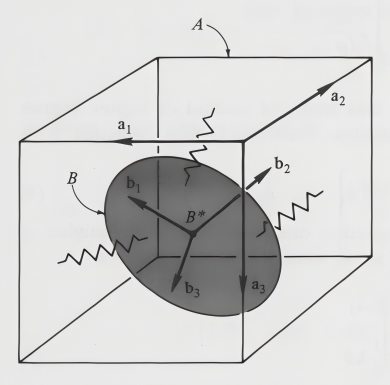
\includegraphics[width=0.8\textwidth]{Figure/小慢旋转.png}
            \caption{缓慢小转动例题}
            \label{fig:缓慢小转动例题}
        \end{figure}
    在图~\ref{fig:缓慢小转动例题} 中，$B$ 表示一个通过弹性支撑连接在航天器 $A$ 上的刚体，航天器 $A$ 在牛顿参考系 $N$ 中的运动方式使得 $A$ 在 $N$ 中的角速度 $\bm{\omega}_{A|N}$ 为
    \begin{equation}
        \bm{\omega}_{A|N} = \omega_1\mathbf{a}_1+\omega_2\mathbf{a}_2+\omega_3\mathbf{a}_3
    \end{equation}
    其中 $\omega_1,\omega_2,\omega_3$ 为常数，$\mathbf{a}_1,\mathbf{a}_2,\mathbf{a}_3$ 为固定在 $A$ 中的一组成右手正交单位向量。$B^*$ 为 $B$ 的质心，$\mathbf{b}_1,\mathbf{b}_2,\mathbf{b}_3$ 为平行于 $B$ 关于 $B^*$ 的惯性主轴的单位向量，相应的转动惯量为 $I_1,I_2,I_3$。

    为建立 $B$ 的运动方程，需要求出 $B$ 相对 $B^*$ 的角动量 $\mathbf{H}$（在 $N$ 中）的一阶时间导数，并假定 $B$ 在 $A$ 中的一切转动都是缓慢小转动。$B$ 在 $A$ 中的姿态用体三转角 $\theta_1,\theta_2,\theta_3$ 描述，当 $\mathbf{a}_i=\mathbf{b}_i$（$i=1,2,3$）时它们均为零。

    $B$ 在 $N$ 中的角速度 $\bm{\omega}_{B|N}$ 可表示为
    \begin{equation}
        \bm{\omega}_{B|N} = \bm{\omega}_{A|N} + \bm{\omega}_{B|A}
        \label{eq:缓慢小转动:角速度合成}
    \end{equation}
    参考式~\eqref{eq:欧拉参数转方向余弦} 和缓慢小转动的结论，可以写出
    \begin{equation}
        \bm{\omega}_{A|N} = (\omega_1+\omega_2\theta_3-\omega_3\theta_2)\mathbf{b}_1
        + (\omega_2+\omega_3\theta_1-\omega_1\theta_3)\mathbf{b}_2
        + (\omega_3+\omega_1\theta_2-\omega_2\theta_1)\mathbf{b}_3
        \label{eq:缓慢小转动:omegaA_N}
    \end{equation}
    并由式~\eqref{eq:缓慢小转动:方向角}，
    \begin{equation}
        \bm{\omega}_{B|A} = \dot{\theta}_1\mathbf{b}_1+\dot{\theta}_2\mathbf{b}_2+\dot{\theta}_3\mathbf{b}_3
        \label{eq:缓慢小转动:omegaB_A}
    \end{equation}
    于是
    \begin{equation}
        \bm{\omega}_{B|N} = (\omega_1+\omega_2\theta_3-\omega_3\theta_2+\dot{\theta}_1)\mathbf{b}_1+\cdots
        \label{eq:缓慢小转动:omegaB_N}
    \end{equation}
    和
    \begin{equation}
        \mathbf{H} = I_1(\omega_1+\omega_2\theta_3-\omega_3\theta_2+\dot{\theta}_1)\mathbf{b}_1+\cdots
        \label{eq:缓慢小转动:角动量}
    \end{equation}
    为求 $\mathbf{H}$ 在 $N$ 中的一阶时间导数，宜利用关系
    \begin{equation}
        \frac{\mathrm{d}\mathbf{H}}{\mathrm{d}t}\Big|_{N} = \frac{\mathrm{d}\mathbf{H}}{\mathrm{d}t}\Big|_{B} + \bm{\omega}_{B|N}\times\mathbf{H}
        \label{eq:缓慢小转动:H导数}
    \end{equation}
    其中
    \begin{equation}
        \frac{\mathrm{d}\mathbf{H}}{\mathrm{d}t}\Big|_{B} = I_1(\omega_2\dot{\theta}_3-\omega_3\dot{\theta}_2+\ddot{\theta}_1)\mathbf{b}_1+\cdots
        \label{eq:缓慢小转动:B系H导数}
    \end{equation}
    而
    \begin{equation}
        \bm{\omega}_{B|N}\times\mathbf{H} = (I_3-I_2)(\omega_2+\omega_3\theta_1-\omega_1\theta_3+\dot{\theta}_2)(\omega_3+\omega_1\theta_2-\omega_2\theta_1+\dot{\theta}_3)\mathbf{b}_1+\cdots
        \label{eq:缓慢小转动:叉积项}
    \end{equation}
    其中一切非线性项都应舍去。于是可得
    \begin{equation}
        \begin{aligned}
            \frac{\mathrm{d}\mathbf{H}}{\mathrm{d}t}\Big|_{N}
            &= \left\{I_1\ddot{\theta}_1+(-I_1-I_2+I_3)\omega_3\dot{\theta}_2-(-I_1+I_2-I_3)\omega_2\dot{\theta}_3\right.\\
            &\quad\left.+(I_3-I_2)[\omega_2\omega_3-(\omega_2^2-\omega_3^2)\theta_1+\omega_1\omega_2\theta_2-\omega_1\omega_3\theta_3]\right\}\mathbf{b}_1+\cdots
        \end{aligned}
        \label{eq:缓慢小转动:H导数结果}
    \end{equation}
\end{example}

%=============================================================
\section{瞬时轴}
\begin{myTheorem}{瞬时轴的性质}
在刚体 $B$ 在参考系 $A$ 中的角速度 $\bm{\omega}$ 为零的瞬时，$B$ 上各点在 $A$ 中的速度彼此相等。只要 $\bm{\omega}$ 不为零，就存在无穷多个 $B$ 上的点，其在 $A$ 中的速度平行于 $\bm{\omega}$ 或等于零。这些点在 $A$ 中具有相同的速度 $\mathbf{v}^*$，它们构成一条平行于 $\bm{\omega}$ 的直线，称为 $B$ 在 $A$ 中的瞬时轴（instantaneous axis）。$\mathbf{v}^*$ 的模长小于 $B$ 上不在瞬时轴上的任意点在 $A$ 中速度的模长。

若 $\mathbf{v}^Q$ 是 $B$ 上任意选取的基点 $Q$ 在 $A$ 中的速度，$P^*$ 是瞬时轴上的点，则 $P^*$ 相对 $Q$ 的位矢 $\mathbf{r}^*$ 可以表示为
\begin{equation}
    \mathbf{r}^* = \frac{\bm{\omega}\times\mathbf{v}^Q}{\bm{\omega}^2} + \mu^*\bm{\omega}
    \label{eq:瞬时轴:r星}
\end{equation}
其中 $\mu^*$ 取决于 $P^*$ 的选取，而 $\mathbf{v}^*$ 由下式给出
\begin{equation}
    \mathbf{v}^* = \frac{\bm{\omega}\cdot\mathbf{v}^Q}{\bm{\omega}^2}\,\bm{\omega}
    \label{eq:瞬时轴:v星}
\end{equation}
\end{myTheorem}

\begin{proof}
        \begin{figure}[H]
            \centering
            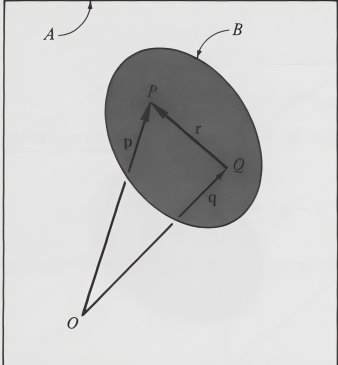
\includegraphics[width=0.8\textwidth]{Figure/瞬时轴.png}
            \caption{瞬时轴的推导}
            \label{fig:瞬时轴推导}
        \end{figure}
    在图~\ref{fig:瞬时轴推导} 中，$P$ 与 $Q$ 均为 $B$ 上任意选取的点，$\mathbf{p}$ 与 $\mathbf{q}$ 分别为它们相对固定在 $A$ 中的点 $O$ 的位矢，$\mathbf{r}$ 为 $P$ 相对 $Q$ 的位矢。于是
    \begin{equation}
        \mathbf{p} = \mathbf{q} + \mathbf{r}
    \end{equation}
    和
    \begin{equation}
        \frac{\mathrm{d}\mathbf{p}}{\mathrm{d}t}\Big|_{A} = \frac{\mathrm{d}\mathbf{q}}{\mathrm{d}t}\Big|_{A} + \frac{\mathrm{d}\mathbf{r}}{\mathrm{d}t}\Big|_{A} = \frac{\mathrm{d}\mathbf{q}}{\mathrm{d}t}\Big|_{A} + \bm{\omega}\times\mathbf{r}
    \end{equation}
    或，由于 $P$ 与 $Q$ 在 $A$ 中的速度 $\mathbf{v}^P$、$\mathbf{v}^Q$ 分别等于 $\frac{\mathrm{d}\mathbf{p}}{\mathrm{d}t}\big|_A$ 与 $\frac{\mathrm{d}\mathbf{q}}{\mathrm{d}t}\big|_A$，
    \begin{equation}
        \mathbf{v}^{P} = \mathbf{v}^{Q} + \bm{\omega}\times\mathbf{r}
    \end{equation}
    若 $\bm{\omega}\neq\bm{0}$，则 $\mathbf{r}$ 总可以表示为与 $\bm{\omega}$ 垂直的向量 $\mathbf{s}$ 与向量 $\mu\bm{\omega}$（$\mu$ 为某个标量）之和，即
    \begin{equation}
        \mathbf{r} = \mathbf{s} + \mu\bm{\omega}
    \end{equation}
    其中
    \begin{equation}
        \bm{\omega}\cdot\mathbf{s} = 0
    \end{equation}
    于是 $\mathbf{v}^{P}$ 可以表示为
    \begin{equation}
        \mathbf{v}^{P} = \mathbf{v}^{Q} + \bm{\omega}\times\mathbf{s}
    \end{equation}
    并且
    \begin{equation}
        \bm{\omega}\times\mathbf{v}^{P} = \bm{\omega}\times\mathbf{v}^{Q} + \bm{\omega}\times(\bm{\omega}\times\mathbf{s}) = \bm{\omega}\times\mathbf{v}^{Q} - \bm{\omega}^2\mathbf{s}
    \end{equation}
    若把 $P$ 取为速度 $\mathbf{v}^*$ 在 $A$ 中平行于 $\bm{\omega}$ 的点 $P^*$，并把相应的 $\mathbf{r},\mathbf{s},\mu$ 记作 $\mathbf{r}^*,\mathbf{s}^*,\mu^*$，则
    \begin{equation}
        0 = \bm{\omega}\times\mathbf{v}^{Q} - \bm{\omega}^2\mathbf{s}^*
    \end{equation}
    \begin{equation}
        \mathbf{r}^* = \mathbf{s}^* + \mu^*\bm{\omega} = \frac{\bm{\omega}\times\mathbf{v}^{Q}}{\bm{\omega}^2} + \mu^*\bm{\omega}
    \end{equation}
    与式~\eqref{eq:瞬时轴:r星} 一致，并且
    \begin{equation}
        \begin{aligned}
            \mathbf{v}^* &= \mathbf{v}^{Q} + \bm{\omega}\times\mathbf{s}^* = \mathbf{v}^{Q} + \frac{\bm{\omega}\times(\bm{\omega}\times\mathbf{v}^{Q})}{\bm{\omega}^2}\\
            &= \frac{\bm{\omega}^2\mathbf{v}^{Q} + \bm{\omega}\cdot\mathbf{v}^{Q}\,\bm{\omega} - \bm{\omega}^2\mathbf{v}^{Q}}{\bm{\omega}^2} = \frac{\bm{\omega}\cdot\mathbf{v}^{Q}}{\bm{\omega}^2}\,\bm{\omega}
        \end{aligned}
    \end{equation}
    与式~\eqref{eq:瞬时轴:v星} 一致。
\end{proof}

\blocksep
\begin{example}
        \begin{figure}[H]
            \centering
            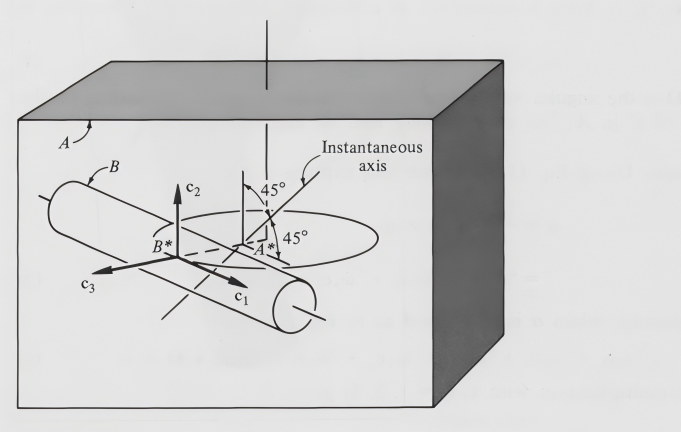
\includegraphics[width=0.8\textwidth]{Figure/瞬时轴例题图.png}
            \caption{瞬时轴例题}
            \label{fig:瞬时轴例题}
        \end{figure}
    在图~\ref{fig:瞬时轴例题} 中，$B$ 表示一个缓慢自旋的圆柱形卫星，其质心 $B^*$ 在固定在参考系 $A$ 中、半径为 $R$ 的圆形轨道上运动。在整个运动过程中，$B$ 的对称轴被约束为始终与圆相切，同时 $B$ 以恒定速率绕该轴转动，使得 $B$ 中一条通过对称轴的平面在 $B^*$ 每绕轨道一周时两次与轨道平面平行。要求确定运动过程中某一典型时刻 $B$ 在 $A$ 中的瞬时轴。

    令 $A^*$ 为 $B^*$ 所在圆的圆心，并取 $C$ 为使圆在 $A^*$ 处的法线与连接 $A^*$、$B^*$ 的直线都固定的参考系，则 $B$ 在 $A$ 中的角速度可以表示为
    \begin{equation}
        \bm{\omega} = \bm{\omega}_{C|A} + \bm{\omega}_{B|C}
        \label{eq:瞬时轴:角速度合成}
    \end{equation}
    进一步，若 $\Omega$ 表示连接 $A^*$、$B^*$ 的直线在 $A$ 中转动的速率，则
    \begin{equation}
        \bm{\omega}_{C|A} = \Omega\,\mathbf{c}_2
        \label{eq:瞬时轴:omegaC_A}
    \end{equation}
    和
    \begin{equation}
        \bm{\omega}_{B|C} = \Omega\,\mathbf{c}_1
        \label{eq:瞬时轴:omegaB_C}
    \end{equation}
    其中 $\mathbf{c}_1$ 与 $\mathbf{c}_2$ 为按图~\ref{fig:瞬时轴例题} 所示方向取的单位向量。于是
    \begin{equation}
        \bm{\omega} = \Omega(\mathbf{c}_1+\mathbf{c}_2)
        \label{eq:瞬时轴:omega}
    \end{equation}
    $B^*$ 在 $A$ 中的速度 $\mathbf{v}^{B^*}$ 为
    \begin{equation}
        \mathbf{v}^{B^*} = R\,\Omega\,\mathbf{c}_1
        \label{eq:瞬时轴:vB星}
    \end{equation}
    因此，若 $P^*$ 是 $B$ 在 $A$ 中的瞬时轴上的点，则 $P^*$ 相对 $B^*$ 的位矢 $\mathbf{r}^*$ 为
    \begin{equation}
        \mathbf{r}^* = \frac{\Omega(\mathbf{c}_1+\mathbf{c}_2)\times(R\,\Omega\,\mathbf{c}_1)}{2\Omega^2} + \mu^*\,\Omega(\mathbf{c}_1+\mathbf{c}_2) = -\frac{R}{2}\,\mathbf{c}_3 + \mu^*\,\Omega(\mathbf{c}_1+\mathbf{c}_2)
        \label{eq:瞬时轴:r星结果}
    \end{equation}
    因此，$B$ 在 $A$ 中的瞬时轴通过连接 $A^*$、$B^*$ 的线段的中点，垂直于 $\mathbf{c}_3$，并与 $\mathbf{c}_1$、$\mathbf{c}_2$ 各成 $45^\circ$ 角，如图~\ref{fig:瞬时轴例题} 所示。
\end{example}

%=============================================================
\section{角加速度}
\begin{myTheorem}{角加速度及其分量关系}
刚体 $B$ 在参考系 $A$ 中的角加速度 $\bm{\alpha}$ 定义为 $B$ 在 $A$ 中的角速度 $\bm{\omega}$（见角速度矢量一节）在 $A$ 中的一阶时间导数：
\begin{equation}
    \bm{\alpha} \triangleq \frac{\mathrm{d}\bm{\omega}}{\mathrm{d}t}\Big|_{A}
    \label{eq:角加速度:定义}
\end{equation}
通常把 $\bm{\omega}$ 与 $\bm{\alpha}$ 都分解为平行于固定在参考系 $C$ 中的单位向量的分量，即把 $\bm{\omega}$ 与 $\bm{\alpha}$ 表示为
\begin{equation}
    \bm{\omega} = \omega_{1|C}\mathbf{c}_1+\omega_{2|C}\mathbf{c}_2+\omega_{3|C}\mathbf{c}_3
    \label{eq:角加速度:omega分量}
\end{equation}
和
\begin{equation}
    \bm{\alpha} = \alpha_{1|C}\mathbf{c}_1+\alpha_{2|C}\mathbf{c}_2+\alpha_{3|C}\mathbf{c}_3
    \label{eq:角加速度:alpha分量}
\end{equation}
其中 $\mathbf{c}_1,\mathbf{c}_2,\mathbf{c}_3$ 组成一组成右手正交单位向量。此时
\begin{equation}
    \alpha_{i|C} = \dot{\omega}_{i|C} + \bm{\Omega}\times\bm{\omega}\cdot\mathbf{c}_i \quad (i=1,2,3)
    \label{eq:角加速度:分量关系}
\end{equation}
其中 $\bm{\Omega}$ 是 $C$ 在 $A$ 中的角速度。换言之，$\alpha_{i|C}$ 是否等于 $\dot{\omega}_{i|C}$，取决于 $C$ 在 $A$ 中的运动。
\end{myTheorem}

\begin{proof}
    利用式~\eqref{eq:角速度矢量:导数关系}，可以把 $\bm{\alpha}$ 表示为
    \begin{equation}
        \bm{\alpha} = \frac{\mathrm{d}\bm{\omega}}{\mathrm{d}t}\Big|_{C} + \bm{\Omega}\times\bm{\omega}
        = \dot{\omega}_{1|C}\mathbf{c}_1+\dot{\omega}_{2|C}\mathbf{c}_2+\dot{\omega}_{3|C}\mathbf{c}_3 + \bm{\Omega}\times\bm{\omega}
    \end{equation}
    因此，当 $\bm{\alpha}$ 按式~\eqref{eq:角加速度:alpha分量} 表达时，
    \begin{equation}
        \alpha_{1|C}\mathbf{c}_1+\alpha_{2|C}\mathbf{c}_2+\alpha_{3|C}\mathbf{c}_3
        = \dot{\omega}_{1|C}\mathbf{c}_1+\dot{\omega}_{2|C}\mathbf{c}_2+\dot{\omega}_{3|C}\mathbf{c}_3 + \bm{\Omega}\times\bm{\omega}
    \end{equation}
    与 $\mathbf{c}_i$（$i=1,2,3$）点乘即得
    \begin{equation}
        \alpha_{i|C} = \dot{\omega}_{i|C} + \bm{\Omega}\times\bm{\omega}\cdot\mathbf{c}_i \quad (i=1,2,3)
    \end{equation}
\end{proof}

\blocksep
\begin{example}
        \begin{figure}[H]
            \centering
            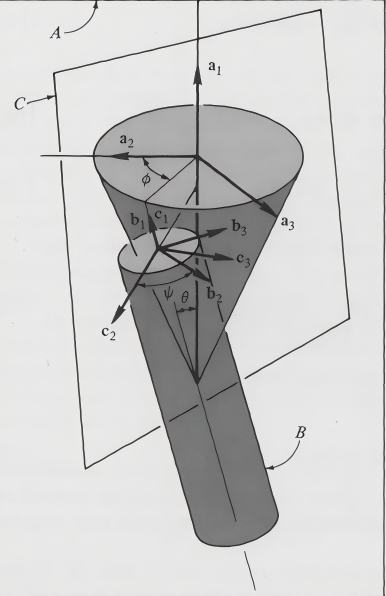
\includegraphics[width=0.8\textwidth]{Figure/角加速度例题图.png}
            \caption{角加速度例题}
            \label{fig:角加速度例题}
        \end{figure}
    图~\ref{fig:角加速度例题} 描绘了第~\ref{sec:angular-velocity-components}~节例题中考虑过的系统。除了以前用过的单位向量外，图中还画出了正交单位向量 $\mathbf{c}_1,\mathbf{c}_2,\mathbf{c}_3$，并标出了使它们固定的参考系 $C$。只考虑 $\dot{\phi}$、$\dot{\psi}$ 以及 $\theta$ 均保持恒定的运动，要求确定量 $\alpha_{i|A}$、$\alpha_{i|B}$ 和 $\alpha_{i|C}$（$i=1,2,3$），它们定义为
    \begin{equation}
        \alpha_{i|A} \triangleq \bm{\alpha}\cdot\mathbf{a}_i,\qquad
        \alpha_{i|B} \triangleq \bm{\alpha}\cdot\mathbf{b}_i,\qquad
        \alpha_{i|C} \triangleq \bm{\alpha}\cdot\mathbf{c}_i \quad (i=1,2,3)
        \label{eq:角加速度:分量定义}
    \end{equation}
    其中 $\bm{\alpha}$ 是 $B$ 在 $A$ 中的角加速度。

    $B$ 在 $A$ 中的角速度 $\bm{\omega}$ 可以表示为
    \begin{equation}
        \bm{\omega} = (\dot{\psi}\,c\theta+\dot{\phi})\mathbf{a}_1 + \dot{\psi}\,s\theta\,c\phi\,\mathbf{a}_2 + \dot{\psi}\,s\theta\,s\phi\,\mathbf{a}_3
        \label{eq:角加速度:omega_a分量}
    \end{equation}
    或
    \begin{equation}
        \bm{\omega} = (\dot{\psi}+\dot{\phi}\,c\theta)\mathbf{b}_1 - \dot{\phi}\,s\theta\,c\psi\,\mathbf{b}_2 + \dot{\phi}\,s\theta\,s\psi\,\mathbf{b}_3
        \label{eq:角加速度:omega_b分量}
    \end{equation}
    或
    \begin{equation}
        \bm{\omega} = (\dot{\psi}+\dot{\phi}\,c\theta)\mathbf{c}_1 - \dot{\phi}\,s\theta\,\mathbf{c}_2
        \label{eq:角加速度:omega_c分量}
    \end{equation}
    在式~\eqref{eq:角加速度:分量关系} 中把 $C$ 换成 $A$，即令 $\bm{\Omega}=0$，参考式~\eqref{eq:角加速度:omega_a分量} 可得
    \begin{equation}
        \alpha_{1|A} = \frac{\mathrm{d}}{\mathrm{d}t}(\dot{\psi}\,c\theta+\dot{\phi}) = 0
    \end{equation}
    \begin{equation}
        \alpha_{2|A} = \frac{\mathrm{d}}{\mathrm{d}t}(\dot{\psi}\,s\theta\,c\phi) = -\dot{\psi}\dot{\phi}\,s\theta\,s\phi
    \end{equation}
    \begin{equation}
        \alpha_{3|A} = \frac{\mathrm{d}}{\mathrm{d}t}(\dot{\psi}\,s\theta\,s\phi) = \dot{\psi}\dot{\phi}\,s\theta\,c\phi
    \end{equation}
    类似地，在式~\eqref{eq:角加速度:分量关系} 中把 $C$ 换成 $B$，即令 $\bm{\Omega}=\bm{\omega}$，由式~\eqref{eq:角加速度:omega_b分量} 可得
    \begin{equation}
        \alpha_{1|B} = \frac{\mathrm{d}}{\mathrm{d}t}(\dot{\psi}+\dot{\phi}\,c\theta) = 0
    \end{equation}
    \begin{equation}
        \alpha_{2|B} = \frac{\mathrm{d}}{\mathrm{d}t}(-\dot{\phi}\,s\theta\,c\psi) = \dot{\phi}\dot{\psi}\,s\theta\,s\psi
    \end{equation}
    \begin{equation}
        \alpha_{3|B} = \frac{\mathrm{d}}{\mathrm{d}t}(\dot{\phi}\,s\theta\,s\psi) = \dot{\phi}\dot{\psi}\,s\theta\,c\psi
    \end{equation}
    最后，由于
    \begin{equation}
        \bm{\Omega} = \bm{\omega}_{C|A} = \dot{\phi}(c\theta\,\mathbf{c}_1-s\theta\,\mathbf{c}_2)
        \label{eq:角加速度:omegaC_A}
    \end{equation}
    从而
    \begin{equation}
        \bm{\Omega}\times\bm{\omega} = \dot{\phi}\dot{\psi}\,s\theta\,\mathbf{c}_3
        \label{eq:角加速度:叉积}
    \end{equation}
    由式~\eqref{eq:角加速度:分量关系} 结合式~\eqref{eq:角加速度:omega_c分量} 和式~\eqref{eq:角加速度:叉积} 可得
    \begin{equation}
        \alpha_{1|C} = \frac{\mathrm{d}}{\mathrm{d}t}(\dot{\psi}+\dot{\phi}\,c\theta) + \dot{\phi}\dot{\psi}\,s\theta\,\mathbf{c}_3\cdot\mathbf{c}_1 = 0
    \end{equation}
    \begin{equation}
        \alpha_{2|C} = \frac{\mathrm{d}}{\mathrm{d}t}(-\dot{\phi}\,s\theta) + \dot{\phi}\dot{\psi}\,s\theta\,\mathbf{c}_3\cdot\mathbf{c}_2 = 0
    \end{equation}
    和
    \begin{equation}
        \alpha_{3|C} = \dot{\phi}\dot{\psi}\,s\theta
    \end{equation}
    因此，除 $\alpha_{3|C}$ 外，式~\eqref{eq:角加速度:分量定义} 中定义的各个量都等于相应角速度测度数的时间导数。
\end{example}

%=============================================================
\section{偏角速度与偏速度}
\begin{myTheorem}{偏角速度与偏速度的唯一表示}
出于后文将说明的原因，当所研究的系统 $S$ 在参考系 $A$ 中的位形用 $n$ 个广义坐标 $q_1,\dots,q_n$ 表征时，往往宜引入 $n$ 个量 $u_1,\dots,u_n$，称为 $S$ 在 $A$ 中的广义速率（generalized speeds），它们是 $\dot{q}_1,\dots,\dot{q}_n$ 的线性组合，形如
\begin{equation}
    u_r \triangleq \sum_{s=1}^{n}Y_{rs}\,\dot{q}_s + Z_r \quad (r=1,\dots,n)
    \label{eq:偏角速度:广义速率}
\end{equation}
其中 $Y_{rs}$ 与 $Z_r$ 是 $q_1,\dots,q_n$ 和 $t$ 的函数，且 $Y_{rs}$（$r,s=1,\dots,n$）的选取使得式~\eqref{eq:偏角速度:广义速率} 可以唯一地解出 $\dot{q}_1,\dots,\dot{q}_n$。此时，属于 $S$ 的刚体 $B$ 在 $A$ 中的角速度 $\bm{\omega}$ 与属于 $S$ 的质点 $P$ 在 $A$ 中的速度 $\mathbf{v}$ 可以唯一地表示为
\begin{equation}
    \bm{\omega} = \sum_{r=1}^{n}\bm{\omega}_r\,u_r + \bm{\omega}_t
    \label{eq:偏角速度:角速度}
\end{equation}
和
\begin{equation}
    \mathbf{v} = \sum_{r=1}^{n}\mathbf{v}_r\,u_r + \mathbf{v}_t
    \label{eq:偏速度:速度}
\end{equation}
其中 $\bm{\omega}_r,\mathbf{v}_r$（$r=1,\dots,n$）、$\bm{\omega}_t$ 与 $\mathbf{v}_t$ 都是 $q_1,\dots,q_n$ 和 $t$ 的函数。向量 $\bm{\omega}_r$ 称为 $B$ 在 $A$ 中的第 $r$ 个偏角速度（partial angular velocity），向量 $\mathbf{v}_r$ 称为 $P$ 在 $A$ 中的第 $r$ 个偏速度（partial velocity），它们可以通过观察式~\eqref{eq:偏角速度:角速度}、\eqref{eq:偏速度:速度} 右端形式直接写出，而不必按式~\eqref{eq:偏角速度:广义速率} 的形式正式引入 $u_1,\dots,u_n$。处理具体问题时，选取广义速率以使系统各刚体角速度与各点速度的表达式尽可能简单，常常不必先显式指定广义坐标。有时也宜对部分或全部 $r$ 取 $u_r=\dot{q}_r$。
\end{myTheorem}

利用广义速率、偏角速度与偏速度可以特别有效地列写广义力的表达式，并能以最少的工作量构造出尽可能简单的运动方程。

\begin{proof}
    对式~\eqref{eq:偏角速度:广义速率} 解出 $\dot{q}_1,\dots,\dot{q}_n$，得
    \begin{equation}
        \dot{q}_s = \sum_{r=1}^{n}W_{sr}\,u_r + X_s \quad (s=1,\dots,n)
        \label{eq:偏角速度:qdot}
    \end{equation}
    其中 $W_{sr}$ 与 $X_s$ 是 $q_1,\dots,q_n$ 和 $t$ 的某个函数。现在，若 $\mathbf{b}_1,\mathbf{b}_2,\mathbf{b}_3$ 组成固定在 $B$ 中的一组成右手正交单位向量，且 $\dot{\mathbf{b}}_i$ 表示 $\mathbf{b}_i$ 在 $A$ 中的一阶时间导数，则
    \begin{equation}
        \dot{\mathbf{b}}_i = \sum_{s=1}^{n}\frac{\partial\mathbf{b}_i}{\partial q_s}\dot{q}_s + \frac{\partial\mathbf{b}_i}{\partial t}
        = \sum_{s=1}^{n}\frac{\partial\mathbf{b}_i}{\partial q_s}\left(\sum_{r=1}^{n}W_{sr}u_r+X_s\right) + \frac{\partial\mathbf{b}_i}{\partial t}
        = \sum_{r=1}^{n}\sum_{s=1}^{n}\frac{\partial\mathbf{b}_i}{\partial q_s}W_{sr}u_r + \sum_{s=1}^{n}\frac{\partial\mathbf{b}_i}{\partial q_s}X_s + \frac{\partial\mathbf{b}_i}{\partial t}
        \quad (i=1,2,3)
    \end{equation}
    其中对 $\mathbf{b}_i$ 的一切偏导数都在 $A$ 中进行。于是（见式~\eqref{eq:角速度矢量:基本关系}）
    \begin{equation}
        \bm{\omega} = \mathbf{b}_1\,\dot{\mathbf{b}}_2\cdot\mathbf{b}_3 + \mathbf{b}_2\,\dot{\mathbf{b}}_3\cdot\mathbf{b}_1 + \mathbf{b}_3\,\dot{\mathbf{b}}_1\cdot\mathbf{b}_2
        = \mathbf{b}_1\left(\sum_{r=1}^{n}\sum_{s=1}^{n}\frac{\partial\mathbf{b}_2}{\partial q_s}\cdot\mathbf{b}_3\,W_{sr}u_r + \sum_{s=1}^{n}\frac{\partial\mathbf{b}_2}{\partial q_s}\cdot\mathbf{b}_3\,X_s + \frac{\partial\mathbf{b}_2}{\partial t}\cdot\mathbf{b}_3\right)
        + \mathbf{b}_2\left(\sum_{r=1}^{n}\sum_{s=1}^{n}\frac{\partial\mathbf{b}_3}{\partial q_s}\cdot\mathbf{b}_1\,W_{sr}u_r + \sum_{s=1}^{n}\frac{\partial\mathbf{b}_3}{\partial q_s}\cdot\mathbf{b}_1\,X_s + \frac{\partial\mathbf{b}_3}{\partial t}\cdot\mathbf{b}_1\right)
        + \mathbf{b}_3\left(\sum_{r=1}^{n}\sum_{s=1}^{n}\frac{\partial\mathbf{b}_1}{\partial q_s}\cdot\mathbf{b}_2\,W_{sr}u_r + \sum_{s=1}^{n}\frac{\partial\mathbf{b}_1}{\partial q_s}\cdot\mathbf{b}_2\,X_s + \frac{\partial\mathbf{b}_1}{\partial t}\cdot\mathbf{b}_2\right)
    \end{equation}
    若定义 $\bm{\omega}_r$ 与 $\bm{\omega}_t$ 为
    \begin{equation}
        \bm{\omega}_r \triangleq \sum_{s=1}^{n}\left(\mathbf{b}_1\frac{\partial\mathbf{b}_2}{\partial q_s}\cdot\mathbf{b}_3 + \mathbf{b}_2\frac{\partial\mathbf{b}_3}{\partial q_s}\cdot\mathbf{b}_1 + \mathbf{b}_3\frac{\partial\mathbf{b}_1}{\partial q_s}\cdot\mathbf{b}_2\right)W_{sr} \quad (r=1,\dots,n)
        \label{eq:偏角速度:偏角速度定义}
    \end{equation}
    和
    \begin{equation}
        \bm{\omega}_t \triangleq \sum_{s=1}^{n}\left(\mathbf{b}_1\frac{\partial\mathbf{b}_2}{\partial q_s}\cdot\mathbf{b}_3 + \mathbf{b}_2\frac{\partial\mathbf{b}_3}{\partial q_s}\cdot\mathbf{b}_1 + \mathbf{b}_3\frac{\partial\mathbf{b}_1}{\partial q_s}\cdot\mathbf{b}_2\right)X_s
        + \mathbf{b}_1\frac{\partial\mathbf{b}_2}{\partial t}\cdot\mathbf{b}_3 + \mathbf{b}_2\frac{\partial\mathbf{b}_3}{\partial t}\cdot\mathbf{b}_1 + \mathbf{b}_3\frac{\partial\mathbf{b}_1}{\partial t}\cdot\mathbf{b}_2
        \label{eq:偏角速度:剩余角速度}
    \end{equation}
    则把式~\eqref{eq:偏角速度:偏角速度定义} 和式~\eqref{eq:偏角速度:剩余角速度} 代入上式即得式~\eqref{eq:偏角速度:角速度}。

    若 $\mathbf{p}$ 为从固定在 $A$ 中的点 $O$ 到 $S$ 的某个质点 $P$ 的位矢，且 $\dot{\mathbf{p}}$ 表示 $\mathbf{p}$ 在 $A$ 中的一阶时间导数，则按定义
    \begin{equation}
        \mathbf{v} \triangleq \dot{\mathbf{p}} = \sum_{s=1}^{n}\frac{\partial\mathbf{p}}{\partial q_s}\dot{q}_s + \frac{\partial\mathbf{p}}{\partial t}
        = \sum_{s=1}^{n}\frac{\partial\mathbf{p}}{\partial q_s}\left(\sum_{r=1}^{n}W_{sr}u_r+X_s\right) + \frac{\partial\mathbf{p}}{\partial t}
        = \sum_{r=1}^{n}\sum_{s=1}^{n}\frac{\partial\mathbf{p}}{\partial q_s}W_{sr}u_r + \sum_{s=1}^{n}\frac{\partial\mathbf{p}}{\partial q_s}X_s + \frac{\partial\mathbf{p}}{\partial t}
    \end{equation}
    因此，定义 $\mathbf{v}_r$ 与 $\mathbf{v}_t$ 为
    \begin{equation}
        \mathbf{v}_r \triangleq \sum_{s=1}^{n}\frac{\partial\mathbf{p}}{\partial q_s}W_{sr} \quad (r=1,\dots,n)
        \label{eq:偏速度:偏速度定义}
    \end{equation}
    和
    \begin{equation}
        \mathbf{v}_t \triangleq \sum_{s=1}^{n}\frac{\partial\mathbf{p}}{\partial q_s}X_s + \frac{\partial\mathbf{p}}{\partial t}
        \label{eq:偏速度:剩余速度}
    \end{equation}
    即得式~\eqref{eq:偏速度:速度}。
\end{proof}

\blocksep
\begin{example}
        \begin{figure}[H]
            \centering
            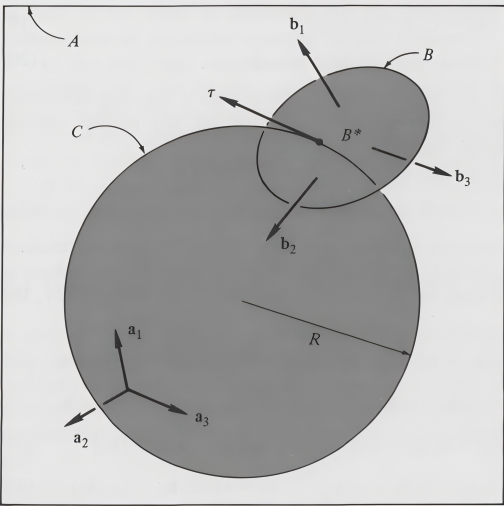
\includegraphics[width=0.8\textwidth]{Figure/偏角速度与偏速度图.png}
            \caption{偏角速度与偏速度例题}
            \label{fig:偏角速度与偏速度例题}
        \end{figure}
    在图~\ref{fig:偏角速度与偏速度例题} 中，$B$ 表示一个刚体，其质心 $B^*$ 以恒定速率 $V$ 在固定在参考系 $A$ 中、半径为 $R$ 的圆形轨道 $C$ 上运动。$\mathbf{a}_1,\mathbf{a}_2,\mathbf{a}_3$ 与 $\mathbf{b}_1,\mathbf{b}_2,\mathbf{b}_3$ 分别为固定在 $A$ 与 $B$ 中的两组成右手正交单位向量，$\bm{\tau}$ 为 $C$ 在 $B^*$ 处的单位切向量。

    由于 $B^*$ 在 $A$ 中的运动是给定的，三个广义坐标足以表征 $B$ 在 $A$ 中的位形。不必显式引入坐标，就可以用 $\mathbf{b}_r$ 与 $B$ 在 $A$ 中的角速度 $\bm{\omega}$ 定义广义速率：
    \begin{equation}
        u_r \triangleq \bm{\omega}\cdot\mathbf{b}_r \quad (r=1,2,3)
        \label{eq:偏角速度:u_r}
    \end{equation}
    由此立即得到
    \begin{equation}
        \bm{\omega} = u_1\mathbf{b}_1+u_2\mathbf{b}_2+u_3\mathbf{b}_3
        \label{eq:偏角速度:omega展开}
    \end{equation}
    比较式~\eqref{eq:偏角速度:角速度} 与式~\eqref{eq:偏角速度:omega展开}，可知 $B$ 在 $A$ 中的偏角速度为
    \begin{equation}
        \bm{\omega}_r = \mathbf{b}_r \quad (r=1,2,3)
        \label{eq:偏角速度:偏角速度结果}
    \end{equation}
    若 $P$ 是 $B$ 上相对 $B^*$ 的位矢为 $r\mathbf{b}_1$ 的点，则 $P$ 在 $A$ 中的速度 $\mathbf{v}$ 可以表示为
    \begin{equation}
        \mathbf{v} = V\bm{\tau} + \bm{\omega}\times(r\mathbf{b}_1) = V\bm{\tau} + r(u_3\mathbf{b}_2-u_2\mathbf{b}_3)
        \label{eq:偏速度:速度展开}
    \end{equation}
    于是 $P$ 在 $A$ 中的偏速度为（比较式~\eqref{eq:偏速度:速度} 与式~\eqref{eq:偏速度:速度展开}）
    \begin{equation}
        \mathbf{v}_1 = 0,\qquad \mathbf{v}_2 = -r\mathbf{b}_3,\qquad \mathbf{v}_3 = r\mathbf{b}_2
        \label{eq:偏速度:偏速度结果}
    \end{equation}

    假设决定用空间三转角 $q_1,q_2,q_3$ 作为广义坐标，把单位向量 $\mathbf{a}_1,\mathbf{a}_2,\mathbf{a}_3$ 与 $\mathbf{b}_1,\mathbf{b}_2,\mathbf{b}_3$ 联系起来（见方向角一节）。则 $\bm{\omega}$ 为（见式~\eqref{eq:方向角角速度:空间三转角}）
    \begin{equation}
        \bm{\omega} = (\dot{q}_1-s_2\dot{q}_3)\mathbf{b}_1 + (c_1\dot{q}_2+s_1c_2\dot{q}_3)\mathbf{b}_2 + (-s_1\dot{q}_2+c_1c_2\dot{q}_3)\mathbf{b}_3
        \label{eq:偏角速度:omega_q}
    \end{equation}
    于是 $u_1,u_2,u_3$ 与 $q_1,q_2,q_3$ 的关系为（见式~\eqref{eq:偏角速度:u_r} 和式~\eqref{eq:偏角速度:omega_q}）
    \begin{equation}
        \begin{aligned}
            u_1 &= \dot{q}_1-s_2\dot{q}_3\\
            u_2 &= c_1\dot{q}_2+s_1c_2\dot{q}_3\\
            u_3 &= -s_1\dot{q}_2+c_1c_2\dot{q}_3
        \end{aligned}
        \label{eq:偏角速度:u_q}
    \end{equation}
    这些方程具有式~\eqref{eq:偏角速度:广义速率} 的形式。注意，列写偏角速度 $\bm{\omega}_r$ 与偏速度 $\mathbf{v}_r$（$r=1,2,3$）的表达式时并不需要使用它们。

    作为式~\eqref{eq:偏角速度:u_r} 的替代，也可以把 $u_r$ 定义为
    \begin{equation}
        u_r \triangleq \dot{q}_r \quad (r=1,2,3)
        \label{eq:偏角速度:u_r替代}
    \end{equation}
    显然这些方程比式~\eqref{eq:偏角速度:u_q} 简单；但当 $u_r$ 这样定义时，$\bm{\omega},\bm{\omega}_r,\mathbf{v},\mathbf{v}_r$（$r=1,2,3$）的表达式往往比采用式~\eqref{eq:偏角速度:u_r} 时复杂。具体地，此时有
    \begin{equation}
        \bm{\omega} = (u_1-s_2u_3)\mathbf{b}_1 + (c_1u_2+s_1c_2u_3)\mathbf{b}_2 + (-s_1u_2+c_1c_2u_3)\mathbf{b}_3
        \label{eq:偏角速度:omega替代}
    \end{equation}
    \begin{equation}
        \bm{\omega}_1 = \mathbf{b}_1,\qquad
        \bm{\omega}_2 = c_1\mathbf{b}_2-s_1\mathbf{b}_3,\qquad
        \bm{\omega}_3 = -s_2\mathbf{b}_1+s_1c_2\mathbf{b}_2+c_1c_2\mathbf{b}_3
        \label{eq:偏角速度:偏角速度替代}
    \end{equation}
    \begin{equation}
        \mathbf{v} = V\bm{\tau} + r[(-s_1u_2+c_1c_2u_3)\mathbf{b}_2-(c_1u_2+s_1c_2u_3)\mathbf{b}_3]
        \label{eq:偏速度:速度替代}
    \end{equation}
    \begin{equation}
        \mathbf{v}_1 = 0,\qquad
        \mathbf{v}_2 = r(-s_1\mathbf{b}_2-c_1\mathbf{b}_3),\qquad
        \mathbf{v}_3 = r(c_1c_2\mathbf{b}_2-s_1c_2\mathbf{b}_3)
        \label{eq:偏速度:偏速度替代}
    \end{equation}
    这些关系取代式~\eqref{eq:偏角速度:omega展开}--\eqref{eq:偏速度:偏速度结果}。
\end{example}
